\documentclass[12pt,a4paper]{article}
\usepackage[utf8]{inputenc}
\usepackage[T1]{fontenc}
\usepackage[brazilian]{babel}
\usepackage{geometry}
\usepackage{graphicx}
\usepackage{amsmath,amssymb}
\usepackage{float}
\usepackage{setspace}
\usepackage{indentfirst}
\usepackage{array}
\usepackage{longtable}
\usepackage{caption}
\usepackage{textcomp}
\usepackage[hidelinks]{hyperref}

% Fonte Arial (Helvetica/Nimbus Sans, equivalente metrico da Arial) e texto todo preto
\usepackage[scaled=0.95]{helvet}
\renewcommand{\familydefault}{\sfdefault}
\captionsetup{font=small,labelfont=bf,labelsep=endash}
\captionsetup[table]{position=top}

\geometry{top=3cm, bottom=2cm, left=3cm, right=2cm}

\onehalfspacing
\setlength{\emergencystretch}{3em}   % evita linhas estouradas com nomes de arquivos longos
% permite quebrar linha depois de "_" (nomes de arquivos longos)
\DeclareRobustCommand{\_}{\textunderscore\allowbreak}
\setlength{\LTpre}{6pt}
\setlength{\LTpost}{6pt}

% codigo e enderecos (D01651, /api/snapshot) em fonte monoespacada que quebra linha
% depois de / . : - = , (evita que caminhos longos vazem da margem)
\ExplSyntaxOn
\tl_new:N \l__cod_tl
\NewDocumentCommand{\cod}{m}
  {
    \tl_set:Nn \l__cod_tl {#1}
    \regex_replace_all:nnN { ([\/\.\:\-\=\,]) } { \1 \c{allowbreak} } \l__cod_tl
    \texttt{\small \tl_use:N \l__cod_tl}
  }
\ExplSyntaxOff

\begin{document}


% ===================== IDENTIFICACAO =====================
\newcommand{\DISCIPLINA}{PGENE586 -- Lean Manufacturing e Qualidade Aplicadas à Indústria 4.0}
\newcommand{\TITULO}{Trabalho Final -- Cenário 25: Sistema de Supervisão Lean para uma Linha de Montagem de Ar-Condicionado de 12 Postos com CLP LS XGK, Gateway Raspberry Pi e Dashboard Web}
\newcommand{\EQUIPE}{Equipe 4 -- Cenário 25}
\newcommand{\AUTORES}{André Ramos \\ Jerry Varela \\ John Guedes \\ Kennedy Madson \\ Lincon Nozawa \\ Renan Barroncas}
\newcommand{\PROFESSOR}{Rafael da Silva Mendonça}
% =========================================================

\begin{titlepage}
    \centering

    % Logo da Universidade
    
\includegraphics[width=3.5cm]{Imagens/ufam-logo.jpg}\\[1cm]

    {\large \textbf{UNIVERSIDADE FEDERAL DO AMAZONAS -- UFAM}} \\[0.3cm]
    {\large \textbf{PROGRAMA DE PÓS-GRADUAÇÃO EM ENGENHARIA ELÉTRICA -- PPGEE}} \\[0.3cm]
    {\large \textbf{Disciplina: \DISCIPLINA}} \\[2cm]

    {\Large \textbf{\TITULO}} \\[2cm]

    \begin{flushleft}
        \textbf{\EQUIPE} \\[0.3cm]
        \textbf{Autores:} \\
        \AUTORES \\[1cm]

        \textbf{Professor:} \\
        \PROFESSOR
    \end{flushleft}

    \vfill

    {\large Manaus -- AM} \\
    {\large \the\year}
\end{titlepage}


\newpage
\tableofcontents
\newpage


\section{Objetivo}

Este trabalho documenta, com evidências de execução, o sistema de supervisão \textit{Lean} desenvolvido pela Equipe 4 para o Cenário 25, uma linha de montagem de ar-condicionado com 12 postos, representada em uma bancada didática. O sistema integra um CLP LS XGK-CPUE, que executa o programa Ladder da linha; uma Raspberry Pi, que atua como \textit{gateway} de borda entre a porta serial do CLP e a rede IP e comanda o motor da esteira; um receptor no Windows, que persiste os eventos e serve a Dashboard web; a Instrução de Trabalho Digital (IT Digital) do posto E07; e um aplicativo Desktop que simula os 12 postos quando o CLP não está disponível. Os objetivos são: (i) descrever a arquitetura e os protocolos de cada enlace; (ii) documentar cada componente - Desktop, Dashboard, Raspberry Pi, CLP, IT Digital e APIs - a partir do código-fonte e da configuração efetivamente usados; e (iii) apresentar, para cada componente, evidências concretas de funcionamento: registros de execução com o CLP real, bancos de dados, testes automatizados, chamadas reais às APIs e capturas de tela.

\subsection{Contexto: Cenário 25 -- linha de montagem de ar-condicionado}

Este é o trabalho final da Equipe 4, responsável pelo Cenário 25 da disciplina: uma linha de montagem de ar-condicionado com 12 postos. A demanda do cenário é de 780 unidades por dia em 450 minutos disponíveis, o que resulta em um Takt time de

\[
\text{Takt} = \frac{450\ \text{min} \times 60\ \text{s/min}}{780\ \text{unidades}} = 34{,}6\ \text{s/unidade}.
\]

O diagnóstico do Módulo I apontou 4 \% de refugo, associado a erros de montagem e à pouca visibilidade do processo, e concentrou a análise do tempo de ciclo no posto E07 (Montagem de Tubulação). No Módulo II, os ciclos e as paradas foram simulados e os aplicativos foram integrados: Simulador da Linha, Andon Digital, Dashboard e IT Digital E07. No Módulo III, documentado neste relatório, a linha é representada por uma bancada didática com CLP e Raspberry Pi, e os mesmos aplicativos passam a receber os dados do processo físico.

Duas ressalvas delimitam a leitura dos resultados. Primeira, os tempos usados nos ensaios (por exemplo, Takt de 60 s no Simulador e meta de 90 peças em 60 min na demonstração) são parâmetros de teste e não representam a demanda do Cenário 25. Segunda, a sequência da IT Digital E07 dura 36 s e ainda precisa ser compatibilizada com a meta de 34 s da E07 e com o Takt de 34,6 s. A referência simulada do Módulo II tem 40 ciclos da E07 (média de 34,0 s e desvio amostral de 0,0 s); a amostra de ciclos físicos para a comparação estatística ainda não foi coletada.

\subsection{Materiais e reprodução}\label{sec:materiais}

O código está organizado em duas aplicações Python. \textbf{hardware/} contém o serviço da Raspberry Pi (Modbus RTU, OPC UA, TCP, SNTP, SQLite e GPIO). \textbf{simulador/} contém o simulador Desktop (PyQt6), o receptor TCP de referência, o cliente OPC UA e a Dashboard web (FastAPI). A documentação do programa Ladder está em \textbf{docs/Documentacao\_Tecnica/DOCUMENTACAO\_CLP\_LS\_XGK.md}, com 21 capturas do projeto \cod{LAB\_NEW\_UPDATED} no XG5000 4.74. Ambiente utilizado nas verificações: Windows 11, Python 3.12.10, PyQt6 6.8.1, asyncua 1.1.5, pymodbus 3.11.3, FastAPI 0.115.11, uvicorn 0.34.0, cryptography 44.0.2 e pytest 8.3.5. Na Raspberry Pi o serviço usa Python 3.11 ou superior, gpiozero 2.0.1 e pigpio 1.78.

As evidências têm três origens, sempre identificadas no texto:

\begin{itemize}
    \item \textbf{Execução real com o CLP} - arquivo \cod{hardware/logs/gateway.log} (32.140 linhas, de 27/09/2026 16:57 a 28/09/2026 13:11) e banco \cod{hardware/data/gateway.db} (18 eventos de Andon capturados no CLP pelo Gateway \cod{LINHA\_A}), além do banco do receptor \cod{simulador/data/reference\_receiver.db} (127 recepções entre 27/09 e 21/11/2026).
    \item \textbf{Testes automatizados} - 98 testes do Simulador e 66 do Gateway, executados em 21/11/2026 (seção 9).
    \item \textbf{Demonstração ponta a ponta com CLP emulado} - para gerar capturas de tela e medições sem o hardware, o Gateway, o receptor e a Dashboard reais foram executados contra um servidor Modbus RTU que reproduz o mapa de registradores do Ladder (\cod{clp\_emulado.py}, descrito na seção 4.6). Os resultados dessa demonstração estão sempre rotulados como ``CLP emulado''. Os bancos e portas da demonstração foram separados dos da instalação (portas 4850, 8091 e 15010), de modo que os dados reais não foram alterados.
\end{itemize}

\section{Arquitetura do sistema}

\subsection{Camadas}

O sistema está organizado em três camadas (Figura \ref{fig:arquitetura}). Na \textbf{camada de campo e controle}, o CLP lê os botões de Andon e os sensores da esteira e executa as máquinas de estados dos 12 postos. No \textbf{gateway de borda}, a Raspberry Pi consulta o CLP por Modbus RTU, guarda os eventos em uma fila SQLite durável, publica a telemetria por OPC UA, entrega os eventos de Andon por TCP e aciona o motor de passo da esteira pelos GPIOs. Na \textbf{supervisão}, o receptor no Windows persiste os eventos, assina a telemetria OPC UA e serve a Dashboard e a IT Digital E07 ao navegador.

\begin{figure}[H]
    \centering
    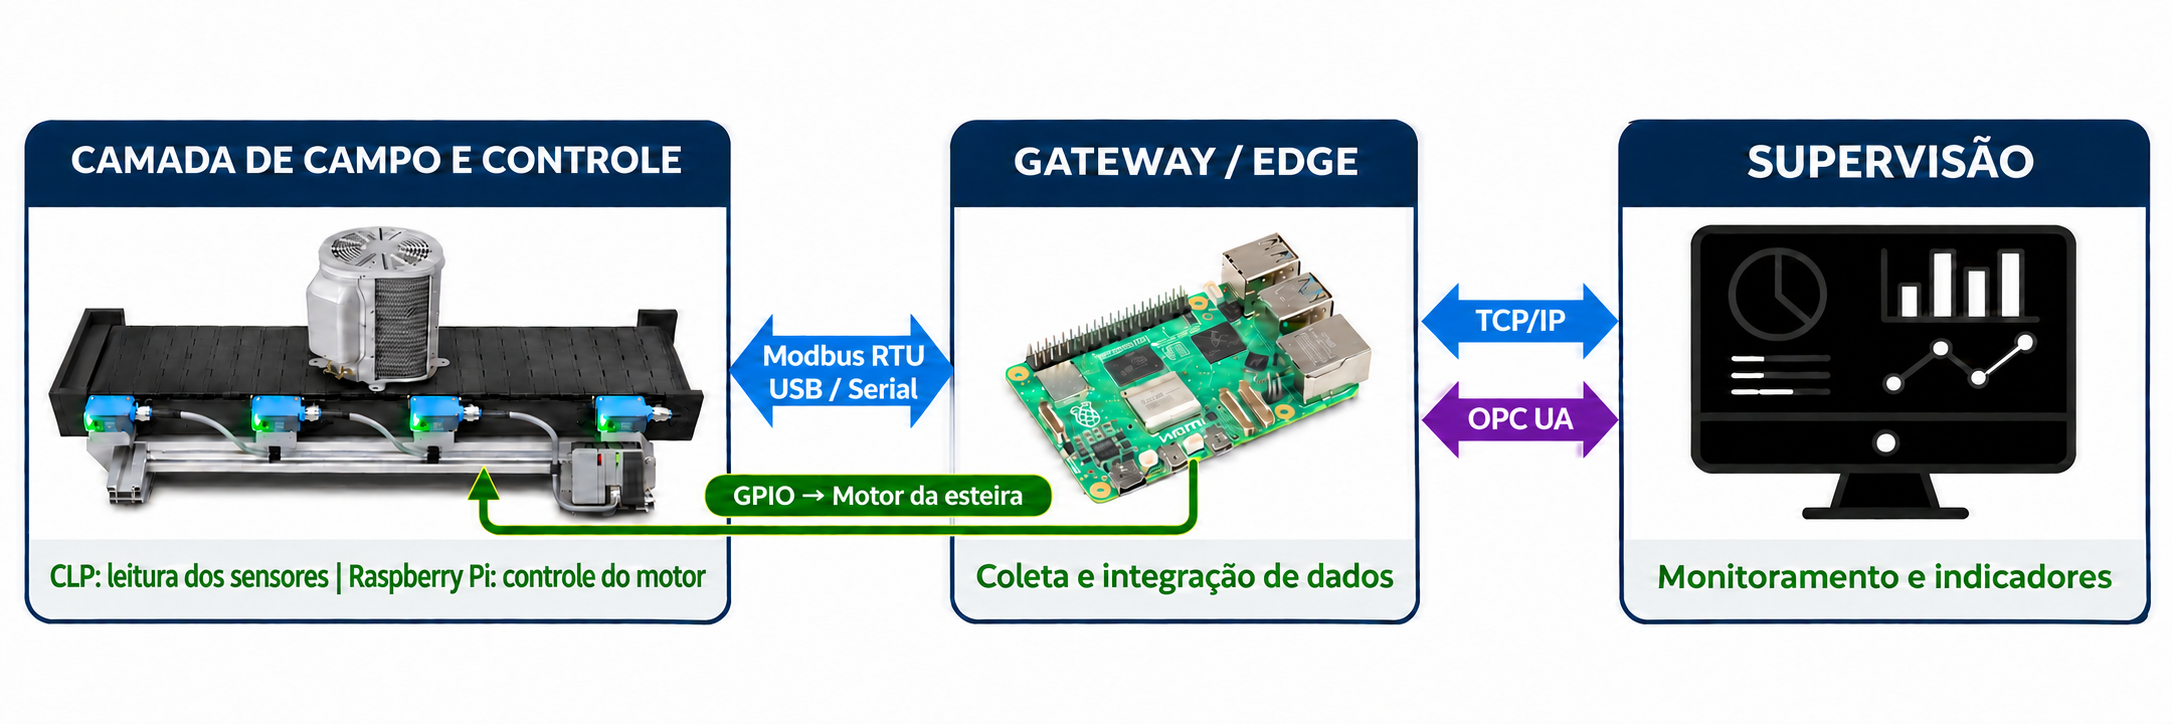
\includegraphics[width=1.00\textwidth]{Imagens/arquitetura_geral.png}
    \caption{Arquitetura em três camadas: campo e controle (CLP, sensores, esteira e motor), gateway de borda (Raspberry Pi) e supervisão (receptor e Dashboard no Windows). (arquivo: docs/Arquiteturas/Arquitetura.pptx)}
    \label{fig:arquitetura}
\end{figure}

\subsection{Enlaces e protocolos}

A Tabela \ref{tab:enlaces} lista os enlaces. A coluna ``Quem inicia'' indica o lado que abre a comunicação; as respostas retornam pelo mesmo enlace.

{\footnotesize
\begin{longtable}{|>{\centering\arraybackslash}p{0.6cm}|>{\raggedright\arraybackslash}p{3.0cm}|>{\raggedright\arraybackslash}p{3.0cm}|>{\raggedright\arraybackslash}p{2.2cm}|>{\raggedright\arraybackslash}p{6.2cm}|}
\caption{Matriz de enlaces da linha (portas do modelo de implantação \cod{hardware/deploy/config.raspberry.toml} e do receptor Windows).}\label{tab:enlaces}\\
\hline
\textbf{Nº} & \textbf{Quem inicia $\rightarrow$ destino} & \textbf{Protocolo} & \textbf{Porta / meio} & \textbf{O que trafega} \\ \hline
\endfirsthead
\hline
\textbf{Nº} & \textbf{Quem inicia $\rightarrow$ destino} & \textbf{Protocolo} & \textbf{Porta / meio} & \textbf{O que trafega} \\ \hline
\endhead
01 & Botões e sensores $\rightarrow$ CLP & Entradas digitais & Bornes de E/S & Níveis lógicos \cod{P00000}-\cod{P0000F} lidos pelo Ladder. \\ \hline
02 & Gateway $\rightarrow$ CLP & Modbus RTU (cliente/servidor) & RS-232 via adaptador USB-RS232, 115200 8N1, estação 1 & Leitura de estados, tempos, Andons, produção e eventos; escrita de ACK, relógio, base de tempos, Start e reset. \\ \hline
03 & Navegador $\rightarrow$ Windows & HTTP e WebSocket & TCP 8081 & Páginas, API REST e JSON em tempo real (\cod{/ws}, \cod{/ws/instruction/e07}). \\ \hline
04 & Gateway $\rightarrow$ receptor & Protocolo binário Andon sobre TCP & TCP 15000 & Evento de 16 bytes; o receptor devolve ACK ASCII de 22 bytes após persistir. \\ \hline
05 & Receptor $\rightarrow$ Gateway & OPC UA (\cod{opc.tcp}) & TCP 4840, \cod{/mock-linha/} & Assinatura de 74 variáveis e chamada de 6 métodos; \cod{Basic256Sha256} com \cod{SignAndEncrypt}. \\ \hline
06 & Gateway $\rightarrow$ servidor de hora & SNTP & UDP 123 & Hora de referência, convertida para \cod{America/Manaus} e gravada no relógio do CLP. \\ \hline
07 & Raspberry Pi $\rightarrow$ DRV8825 & GPIO & STEP BCM 18, DIR BCM 25, EN BCM 15 & Pulsos de passo, sentido e habilitação (EN ativo em nível baixo). \\ \hline
08 & DRV8825 $\rightarrow$ motor & Acionamento elétrico & Bobinas & Corrente controlada pelo driver. \\ \hline
\end{longtable}
}

\subsection{Fluxos principais}

\textbf{Entrega de um Andon.} (1) O operador aciona o botão; o Ladder grava oito palavras na FIFO \cod{D00300} e publica o evento em \cod{D00101}-\cod{D00108}, com a quantidade pendente em \cod{D00100}. (2) O Gateway lê o bloco por Modbus (FC04), grava os 16 bytes no SQLite com \cod{synchronous=FULL} e só então aciona \cod{P10000} (FC05). (3) O CLP retira o evento da fila. (4) O Gateway abre uma conexão TCP com o receptor e envia os 16 bytes; o receptor persiste e responde com o ACK de 22 bytes; só então o evento é marcado como confirmado. Os dois ACKs (\cod{P10000} e TCP) ocorrem em enlaces e momentos diferentes e garantem, respectivamente, que o Gateway guardou o evento e que o receptor o persistiu.

\textbf{Supervisão ao vivo.} O Gateway lê a cada 250 ms os Andons, Takt time, último ciclo, os 12 estados (\cod{D01651}-\cod{D01662}) e o contador de produção (\cod{D16052}) e publica as alterações no OPC UA. O receptor recebe as notificações por assinatura e a Dashboard envia o estado consolidado ao navegador a cada 1 s pelo WebSocket \cod{/ws}.

\textbf{Comandos do operador.} Os botões da Dashboard chamam a API HTTP do receptor, que chama métodos OPC UA do Gateway, que escreve no CLP por Modbus (Tabela \ref{tab:comandos}).

{\footnotesize
\begin{longtable}{|>{\raggedright\arraybackslash}p{2.0cm}|>{\raggedright\arraybackslash}p{3.6cm}|>{\raggedright\arraybackslash}p{3.6cm}|>{\raggedright\arraybackslash}p{5.6cm}|}
\caption{Caminho de cada comando do operador até o CLP.}\label{tab:comandos}\\
\hline
\textbf{Ação} & \textbf{Navegador $\rightarrow$ API} & \textbf{Receptor $\rightarrow$ Gateway (OPC UA)} & \textbf{Gateway $\rightarrow$ CLP (Modbus RTU)} \\ \hline
\endfirsthead
\hline
\textbf{Ação} & \textbf{Navegador $\rightarrow$ API} & \textbf{Receptor $\rightarrow$ Gateway (OPC UA)} & \textbf{Gateway $\rightarrow$ CLP (Modbus RTU)} \\ \hline
\endhead
Importar base & \cod{POST /api/process/cycle-base} & \cod{Linha/CarregarBaseCiclos} & FC16 grava 288 palavras em 12 blocos (\cod{D17001}-\cod{D17288}) e FC03 confere cada bloco. \\ \hline
Start & \cod{POST /api/process/start} & \cod{Linha/IniciarSimulacao} & FC05 pulsa \cod{P10002} por 2 s; a confirmação é um posto no estado 2. \\ \hline
Limpar base & \cod{POST /api/process/clear-base} & \cod{Linha/LimparBase} & FC05 pulsa \cod{P10003} por 2 s; o Gateway confere \cod{D16052 = 0}. \\ \hline
\end{longtable}
}

\section{CLP LS XGK-CPUE (item 2d)}

\subsection{Organização do programa Ladder}

O CLP executa o projeto \cod{LAB\_NEW\_UPDATED}, editado no XG5000 versão 4.74 (Figuras \ref{fig:clp01} e \ref{fig:clp02}). O projeto tem dois programas de varredura e uma sub-rotina:

\begin{itemize}
    \item \textbf{BUTTONS} - trata as bordas das 12 entradas de botão \cod{P00000}-\cod{P0000B} em um único registrador de estados, \cod{D01501}, e gera as marcas internas \cod{M00020} em diante;
    \item \textbf{ANDON} - lê o relógio (\cod{DATERD}), serve a fila de comunicação com o Gateway, aplica o relógio recebido (\cod{DATEWRP}), executa as máquinas de estados dos 12 postos e gera o comando do motor;
    \item \textbf{MENSAGEM\_ANDON} - sub-rotina que grava cada evento, em oito palavras, na FIFO \cod{D00300} com \cod{FIWR}.
\end{itemize}

\begin{figure}[H]
    \centering
    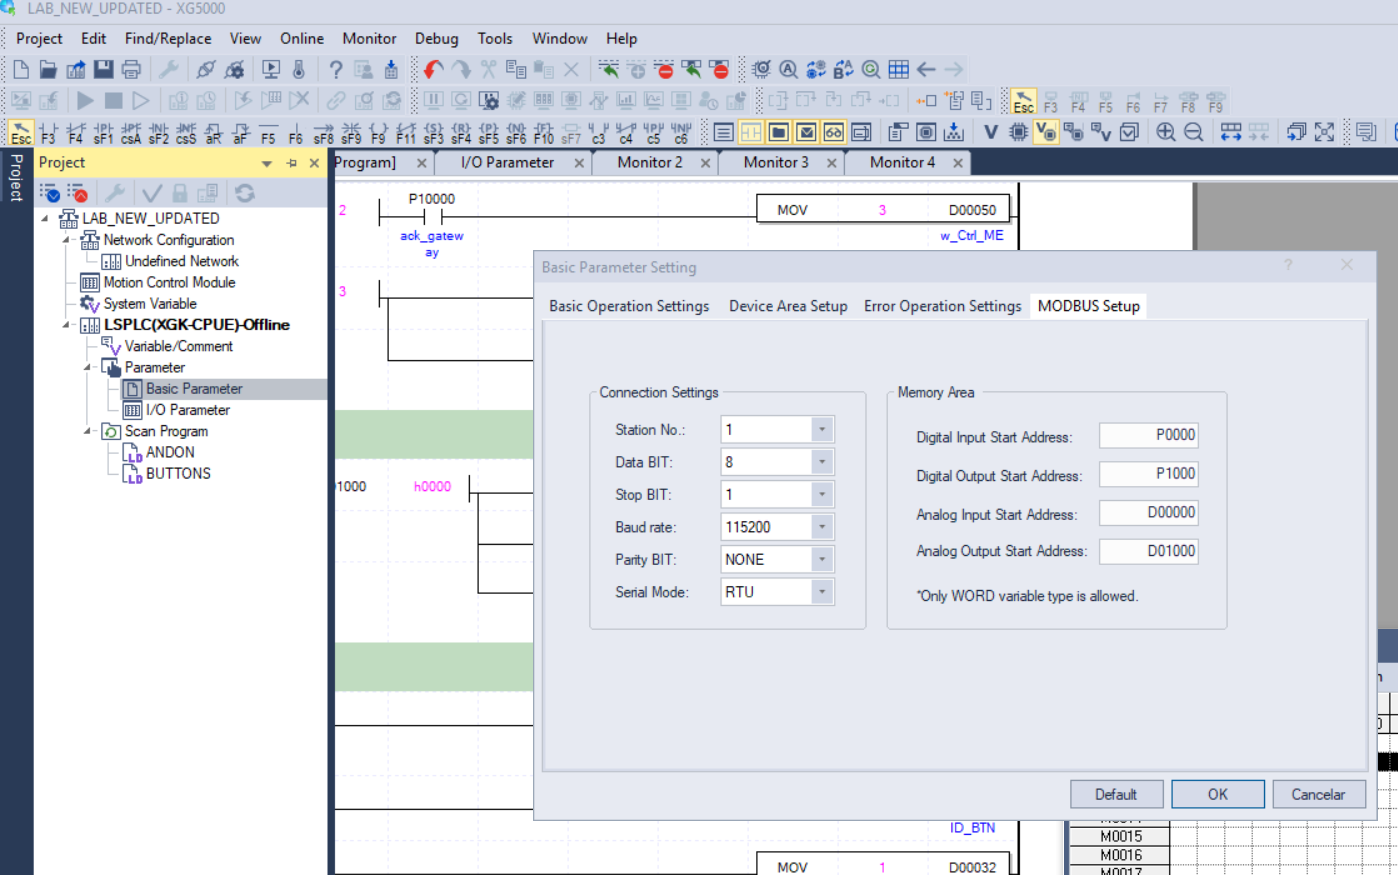
\includegraphics[width=0.80\textwidth]{Imagens/clp_01_configuracao_modbus.png}
    \caption{XG5000, \textit{Basic Parameter} $\rightarrow$ \textit{MODBUS Setup}: estação 1, 115200 baud, 8 bits, sem paridade, 1 bit de parada, modo RTU; áreas \cod{P0000}, \cod{P1000}, \cod{D00000} e \cod{D01000}. (arquivo: Imagens/clp\_01\_configuracao\_modbus.png)}
    \label{fig:clp01}
\end{figure}

\begin{figure}[H]
    \centering
    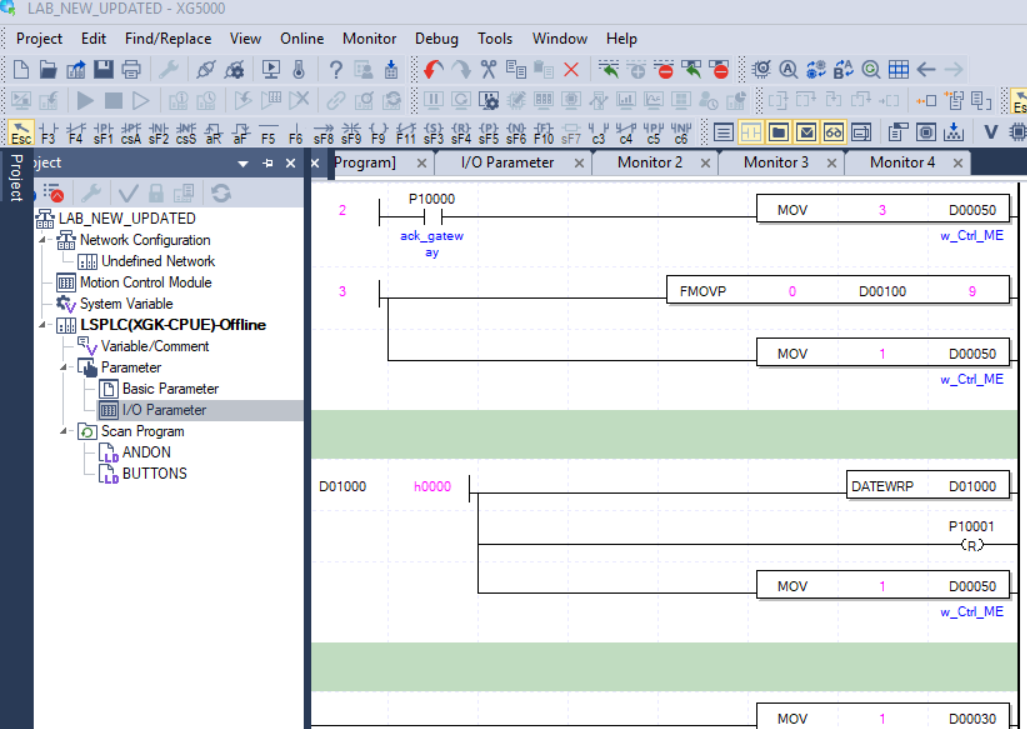
\includegraphics[width=0.62\textwidth]{Imagens/clp_02_arvore_projeto.png}
    \caption{Árvore do projeto \cod{LAB\_NEW\_UPDATED} com a CPU XGK-CPUE e os programas ANDON e BUTTONS em \textit{Scan Program}. (arquivo: Imagens/clp\_02\_arvore\_projeto.png)}
    \label{fig:clp02}
\end{figure}

\subsection{Mapa Modbus}

O Gateway é o cliente Modbus RTU e o CLP é o servidor. A Tabela \ref{tab:mapa} é o mapa efetivamente configurado em \cod{hardware/deploy/config.raspberry.toml}. O endereço Modbus tem base zero dentro de cada área; a área de \textit{Holding Registers} começa em \cod{D01000} e a de \textit{Input Registers} em \cod{D00000}, por isso \cod{D16052} corresponde ao \textit{holding register} 15052.

{\footnotesize
\begin{longtable}{|>{\raggedright\arraybackslash}p{2.6cm}|>{\raggedright\arraybackslash}p{2.9cm}|>{\centering\arraybackslash}p{1.9cm}|>{\raggedright\arraybackslash}p{7.2cm}|}
\caption{Mapa Modbus entre o Gateway e o CLP.}\label{tab:mapa}\\
\hline
\textbf{XG5000} & \textbf{Área / função} & \textbf{Endereço} & \textbf{Conteúdo} \\ \hline
\endfirsthead
\hline
\textbf{XG5000} & \textbf{Área / função} & \textbf{Endereço} & \textbf{Conteúdo} \\ \hline
\endhead
\cod{D00100} & Input Reg., FC04 & 100 & Palavras pendentes na fila (0, 8, 16...). \\ \hline
\cod{D00101}-\cod{D00108} & Input Reg., FC04 & 101-108 & Evento de 16 bytes; \cod{D00101 = 1}. \\ \hline
\cod{D00109}-\cod{D00111} & Input Reg., FC04 & 109-111 & Estado instantâneo dos Andons, 4 postos por palavra, 1 bit por categoria. \\ \hline
\cod{D00112} & Input Reg., FC04 & 112 & Comando do motor: 1 ligado, 0 desligado. \\ \hline
\cod{D00113}-\cod{D00160} & Input Reg., FC04 & 113-160 & Por posto, Takt time e último ciclo em UInt32 (palavra baixa primeiro, décimos de segundo). \\ \hline
\cod{D01000}-\cod{D01003} & Holding Reg., FC16 & 0-3 & Relógio em BCD para \cod{DATEWRP}. \\ \hline
\cod{D01200} & Holding Reg., FC03/FC06 & 200 & Velocidade do motor, 0 a 100 \%. \\ \hline
\cod{D01201.0} & Holding Reg., FC03/FC06 & 201, bit 0 & Pedido de parada da linha. \\ \hline
\cod{D01651}-\cod{D01662} & Holding Reg., FC03 & 651-662 & Estado dos postos P01 a P12 (0 a 3). \\ \hline
\cod{D16052} & Holding Reg., FC03 & 15052 & Contador de produção (peças concluídas no P12). \\ \hline
\cod{D17001}-\cod{D17288} & Holding Reg., FC16/FC03 & 16001-16288 & Base de tempos: 24 palavras por posto. \\ \hline
\cod{P10000} & Coil, FC05 & 0 & ACK do evento lido pelo Gateway. \\ \hline
\cod{P10001} & Coil, FC05 & 1 & Pedido de aplicação do relógio. \\ \hline
\cod{P10002} & Coil, FC05 & 2 & Pulso de Start (2 s). \\ \hline
\cod{P10003} & Coil, FC05 & 3 & Pulso de reset dos postos (2 s). \\ \hline
\end{longtable}
}

\subsection{Botões e geração dos eventos de Andon}

O programa BUTTONS usa um único registrador para as 12 entradas. \cod{D01501} parte de 100 e, para a entrada de posição \textit{n} (1 a 12), percorre \cod{100} $\rightarrow$ \textit{n} (borda de descida) $\rightarrow$ \textit{n}+12 (subida) $\rightarrow$ \textit{n}+24 (descida) $\rightarrow$ \cod{100} (subida). Os três estados intermediários mantêm ativa a marca do botão (para \cod{P00000}, \cod{M00020} ativa em 1, 13 e 25). Cada borda da marca dispara, no programa ANDON, o preenchimento de posto (\cod{D00030}), botão (\cod{D00031}) e estado (\cod{D00032}: 1 ligado, 2 desligado) e chama \cod{MENSAGEM\_ANDON}, que enfileira tipo, posto, data e hora (lidos por \cod{DATERD} em \cod{D00040}-\cod{D00043}), botão e estado (Figura \ref{fig:clp13}).

A entrega ao Gateway é controlada por \cod{D00050} (Figuras \ref{fig:clp09} e \ref{fig:clp10}): em \textbf{1}, se a FIFO não está vazia, o Ladder copia o cabeçalho para \cod{D00100} e retira as oito palavras para \cod{D00101}-\cod{D00108} com \cod{FIFRDP}; em \textbf{2}, mantém o evento disponível até o Gateway ligar \cod{P10000}; em \textbf{3}, zera as nove palavras com \cod{FMOVP} e volta a 1.

\begin{figure}[H]
    \centering
    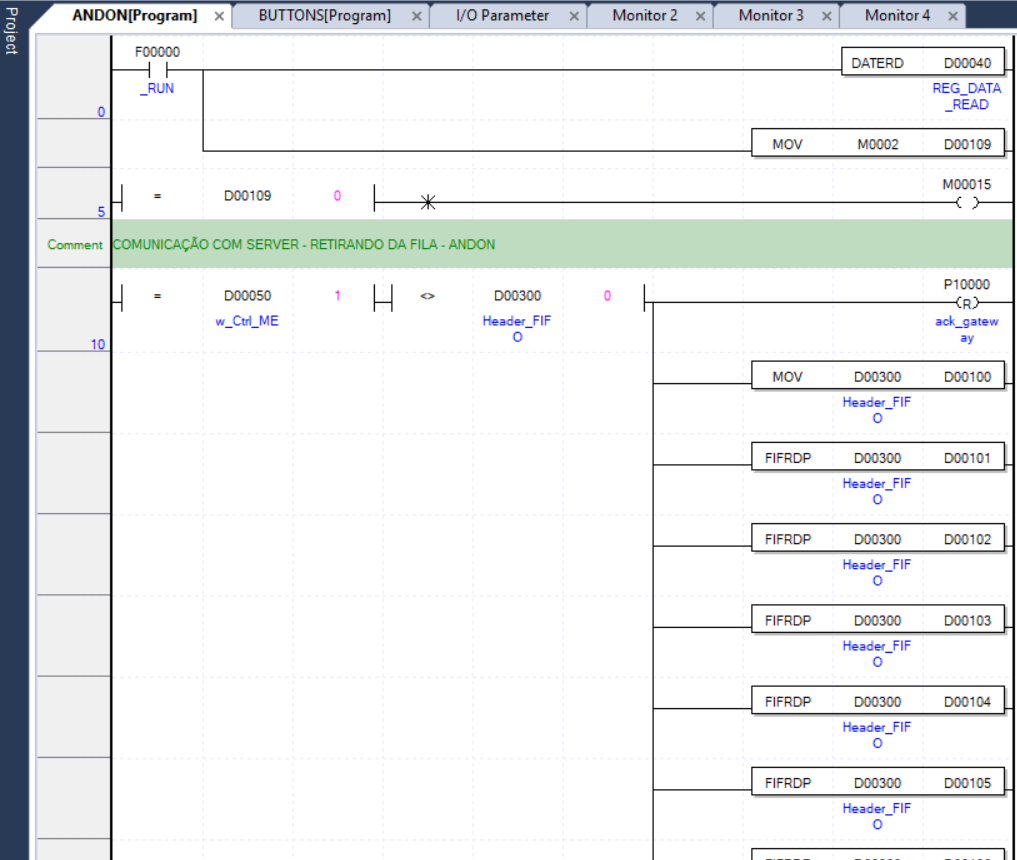
\includegraphics[width=0.78\textwidth]{Imagens/clp_09_andon_leitura_fila.png}
    \caption{Programa ANDON: \cod{DATERD} em \cod{D00040} e início da retirada da FIFO \cod{D00300} para \cod{D00100}-\cod{D00108} quando \cod{D00050 = 1}. (arquivo: Imagens/clp\_09\_andon\_leitura\_fila.png)}
    \label{fig:clp09}
\end{figure}

\begin{figure}[H]
    \centering
    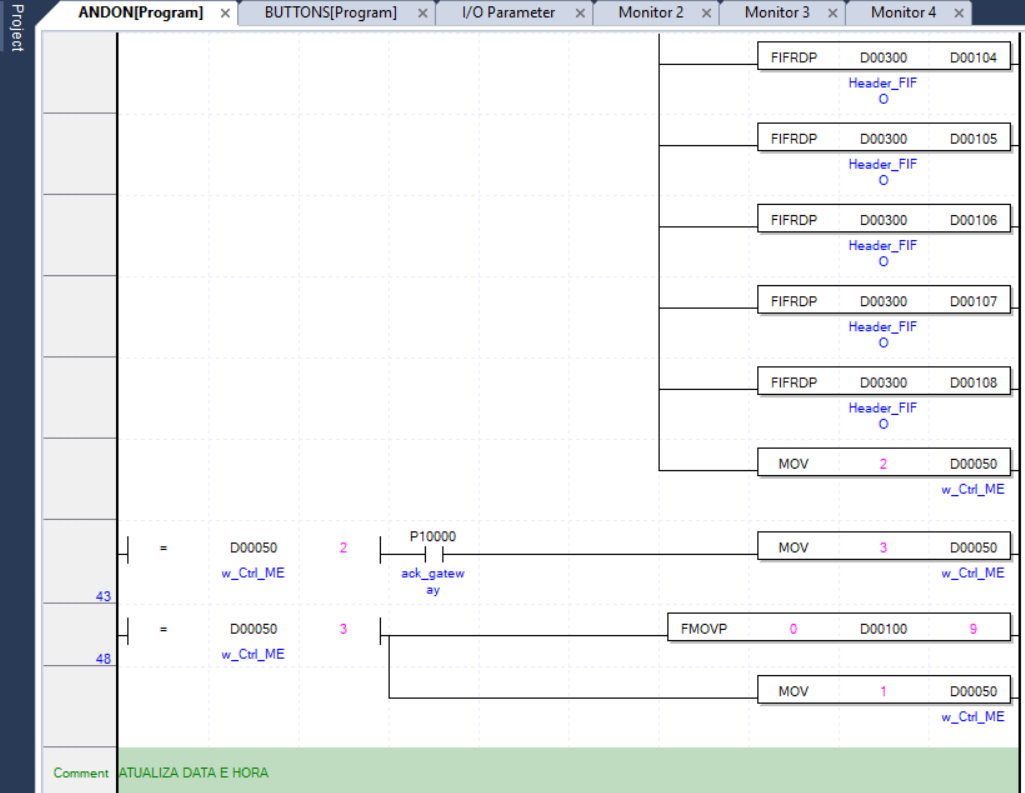
\includegraphics[width=0.78\textwidth]{Imagens/clp_10_andon_ack_gateway.png}
    \caption{Fim da retirada (\cod{MOV 2 D00050}), espera do ACK \cod{P10000} (\cod{MOV 3 D00050}) e limpeza do bloco com \cod{FMOVP 0 D00100 9}. (arquivo: Imagens/clp\_10\_andon\_ack\_gateway.png)}
    \label{fig:clp10}
\end{figure}

\begin{figure}[H]
    \centering
    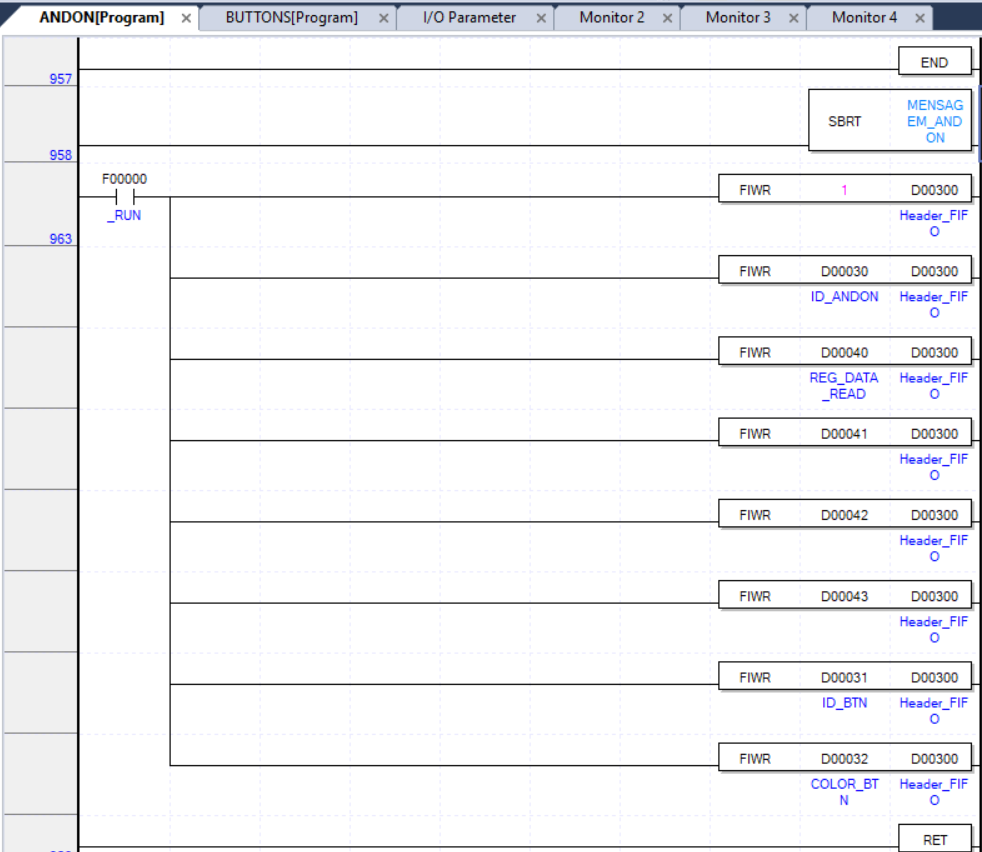
\includegraphics[width=0.78\textwidth]{Imagens/clp_13_andon_gravacao_fila.png}
    \caption{Sub-rotina \cod{MENSAGEM\_ANDON}: sete \cod{FIWR} gravam na FIFO \cod{D00300} o tipo, o posto, as quatro palavras de data e hora, o botão e o estado. (arquivo: Imagens/clp\_13\_andon\_gravacao\_fila.png)}
    \label{fig:clp13}
\end{figure}

\subsection{Máquinas de estados dos postos}

Cada posto tem uma palavra de estado (\cod{D01651} a \cod{D01662}): \textbf{0} espera, \textbf{1} preparação, \textbf{2} medição (processando) e \textbf{3} fim do ciclo. Nos postos 01 e 02, a passagem 2 $\rightarrow$ 3 ocorre no fim do temporizador cujo \textit{preset} é o tempo da base (\cod{D17001[Z001]}, \cod{D17025[Z002]}); no P07, manual, ocorre na borda de \cod{P0000D}. Os postos automáticos 08 a 10 vão direto de 0 para 2 quando o sensor de entrada confirma a peça e encerram a medição na borda do sensor seguinte. Na passagem 3 $\rightarrow$ 0 o Ladder copia o tempo medido para o bloco de telemetria (\cod{D00115}, \cod{D00119}, ..., \cod{D00151}), incrementa o contador do posto (\cod{D16041}-\cod{D16050}) e habilita o posto seguinte. A borda de \cod{P10002} ativa \cod{M00101}, entrada do P01 (Start); \cod{P10003} zera estados, temporizadores e contadores (reset). O motor é ligado (\cod{D00112.0}) quando \cod{D01501 = 100}, isto é, nenhum Andon pressionado, e algum dos postos 08 a 10 está em estado diferente de 0 (Figuras \ref{fig:clp15}, \ref{fig:clp17} e \ref{fig:clp21}).

\begin{figure}[H]
    \centering
    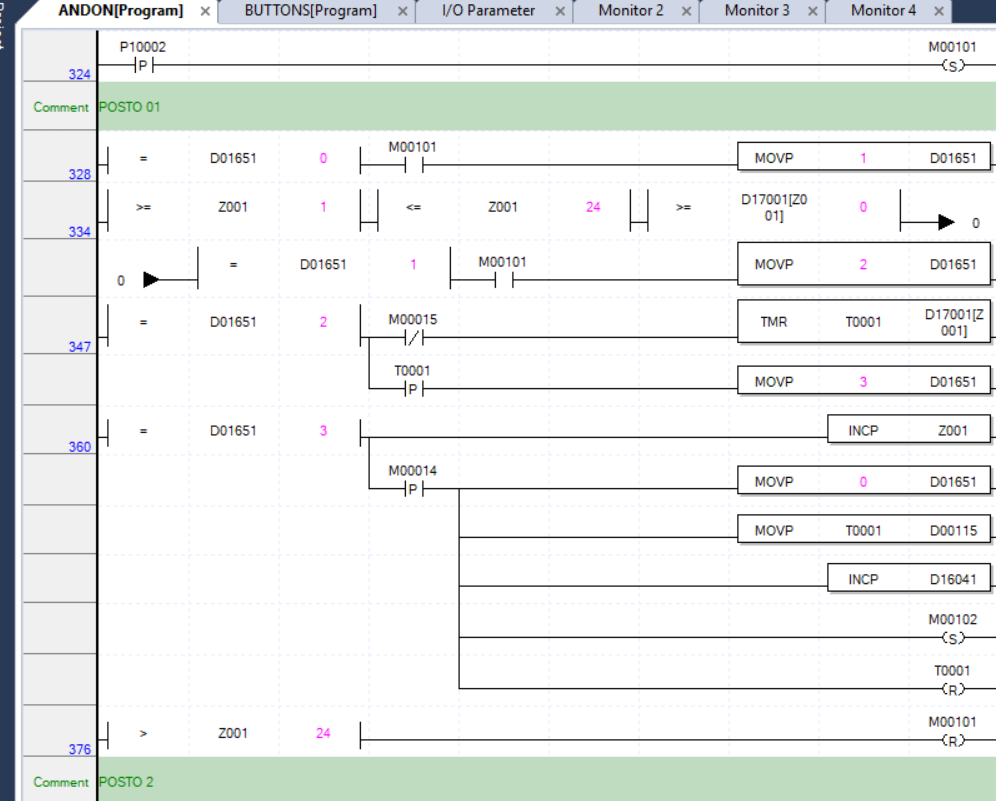
\includegraphics[width=0.78\textwidth]{Imagens/clp_15_posto_01.png}
    \caption{Posto 01: estado em \cod{D01651}, temporizador \cod{T0001} com \textit{preset} indexado \cod{D17001[Z001]}, cópia do tempo para \cod{D00115} e incremento de \cod{D16041}. (arquivo: Imagens/clp\_15\_posto\_01.png)}
    \label{fig:clp15}
\end{figure}

\begin{figure}[H]
    \centering
    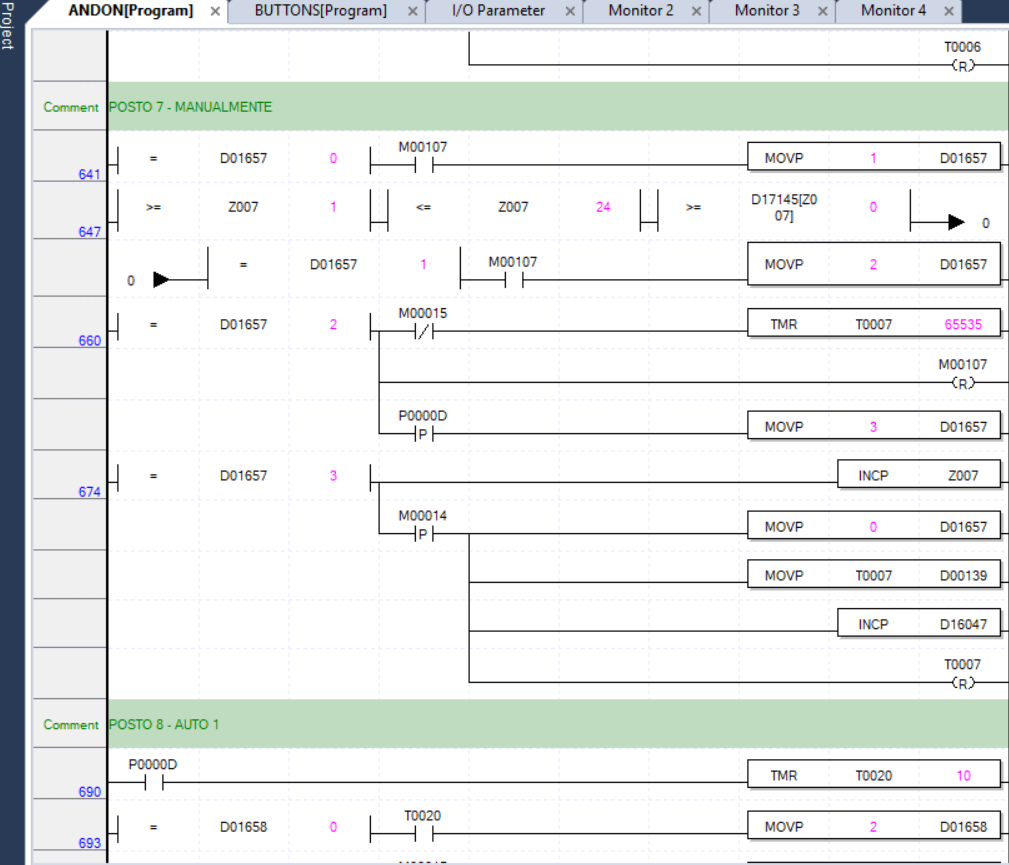
\includegraphics[width=0.78\textwidth]{Imagens/clp_17_posto_07_manual.png}
    \caption{Posto 07 (manual): estado em \cod{D01657}; a borda de \cod{P0000D} leva ao estado 3. É a transição 1 $\rightarrow$ 2 deste posto que sincroniza a IT Digital E07 (seção 7). (arquivo: Imagens/clp\_17\_posto\_07\_manual.png)}
    \label{fig:clp17}
\end{figure}

\begin{figure}[H]
    \centering
    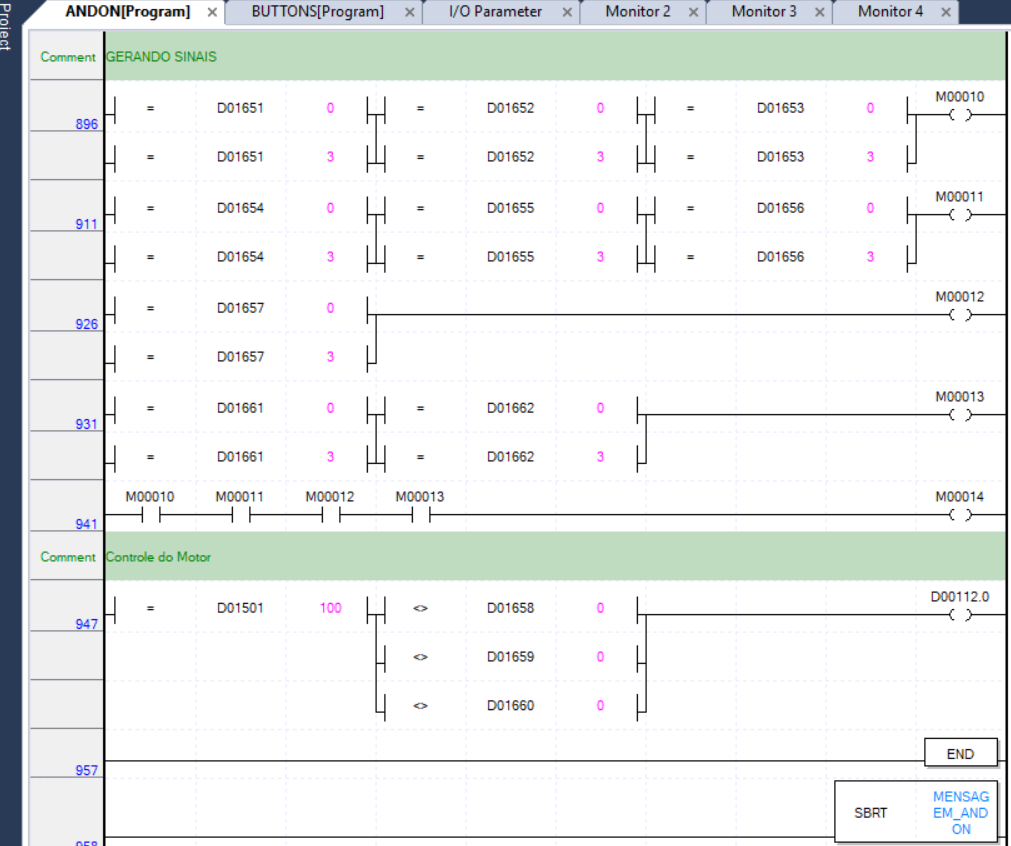
\includegraphics[width=0.78\textwidth]{Imagens/clp_21_sinais_e_motor.png}
    \caption{Geração de \cod{M00014} a partir de \cod{M00010}-\cod{M00013} e condição da saída \cod{D00112.0} (comando do motor). (arquivo: Imagens/clp\_21\_sinais\_e\_motor.png)}
    \label{fig:clp21}
\end{figure}

As demais 13 capturas do XG5000 estão no Anexo (Figuras A1 a A13).

\subsection{Evidência: eventos reais lidos do CLP}

Em 27/09/2026 o Gateway \cod{LINHA\_A} foi executado com o CLP real ligado à porta COM10 por um adaptador USB-RS232. O banco \cod{hardware/data/gateway.db} registra 18 eventos de Andon, todos do posto P05 (o botão cabeado na bancada): 6 de Processo, 6 de Equipamento, 4 de Qualidade e 2 de Material, sempre em pares ligado/desligado. A Tabela \ref{tab:decode} decodifica, byte a byte, o primeiro evento tal como o CLP o publicou em \cod{D00101}-\cod{D00108}.

{\footnotesize
\begin{longtable}{|>{\centering\arraybackslash}p{1.4cm}|>{\centering\arraybackslash}p{1.9cm}|>{\raggedright\arraybackslash}p{3.4cm}|>{\raggedright\arraybackslash}p{7.6cm}|}
\caption{Decodificação do evento 1 de \cod{gateway.db} (\cod{event\_uid} \cod{LINHA\_A-20260927165903-3DE06210}). Bytes em hexadecimal: \cod{00 01 00 05 09 26 16 27 03 59 20 00 00 03 00 01}.}\label{tab:decode}\\
\hline
\textbf{Bytes} & \textbf{Valor (hex)} & \textbf{Campo} & \textbf{Interpretação} \\ \hline
\endfirsthead
\hline
\textbf{Bytes} & \textbf{Valor (hex)} & \textbf{Campo} & \textbf{Interpretação} \\ \hline
\endhead
0-1 & \cod{00 01} & Tipo & 1 = evento de Andon gerado pelo CLP (\cod{D00101}). \\ \hline
2-3 & \cod{00 05} & Posto & P05. \\ \hline
4 / 5 & \cod{09} / \cod{26} & Mês / ano (BCD) & Setembro de (20)26. \\ \hline
6 / 7 & \cod{16} / \cod{27} & Hora / dia (BCD) & 16 h, dia 27. \\ \hline
8 / 9 & \cod{03} / \cod{59} & Segundo / minuto (BCD) & 59 min 03 s. \\ \hline
10 / 11 & \cod{20} / \cod{00} & Século / dia da semana & Século 20; dia da semana 0 = domingo (27/09/2026 foi domingo). \\ \hline
12-13 & \cod{00 03} & Botão & 3 = Processo (Andon verde). \\ \hline
14-15 & \cod{00 01} & Estado & 1 = ligado. \\ \hline
\end{longtable}
}

O resultado, ``P05, Processo, ligado, 27/09/2026 16:59:03'', coincide com as colunas \cod{station}, \cod{button\_id}, \cod{status} e \cod{occurred\_at} gravadas pelo Gateway e com a linha correspondente do receptor (\cod{reception}, primeira recepção, às 16:59:04,04). O identificador do evento combina o Gateway, o carimbo de tempo do pacote e o CRC32 dos 16 bytes. A lista completa dos 18 eventos está na Tabela A1 do Anexo.

A Figura \ref{fig:latencia} mostra, para cada evento, o tempo entre a gravação no SQLite e o ACK \cod{P10000} escrito no CLP e, em seguida, até o ACK TCP do receptor. O ACK no CLP levou entre 13,4 e 17,3 ms (mediana 15,9 ms) e a entrega completa, entre 23,4 e 39,9 ms (mediana 33,9 ms). Nenhum evento precisou de nova tentativa (\cod{attempts = 0}).

\begin{figure}[H]
    \centering
    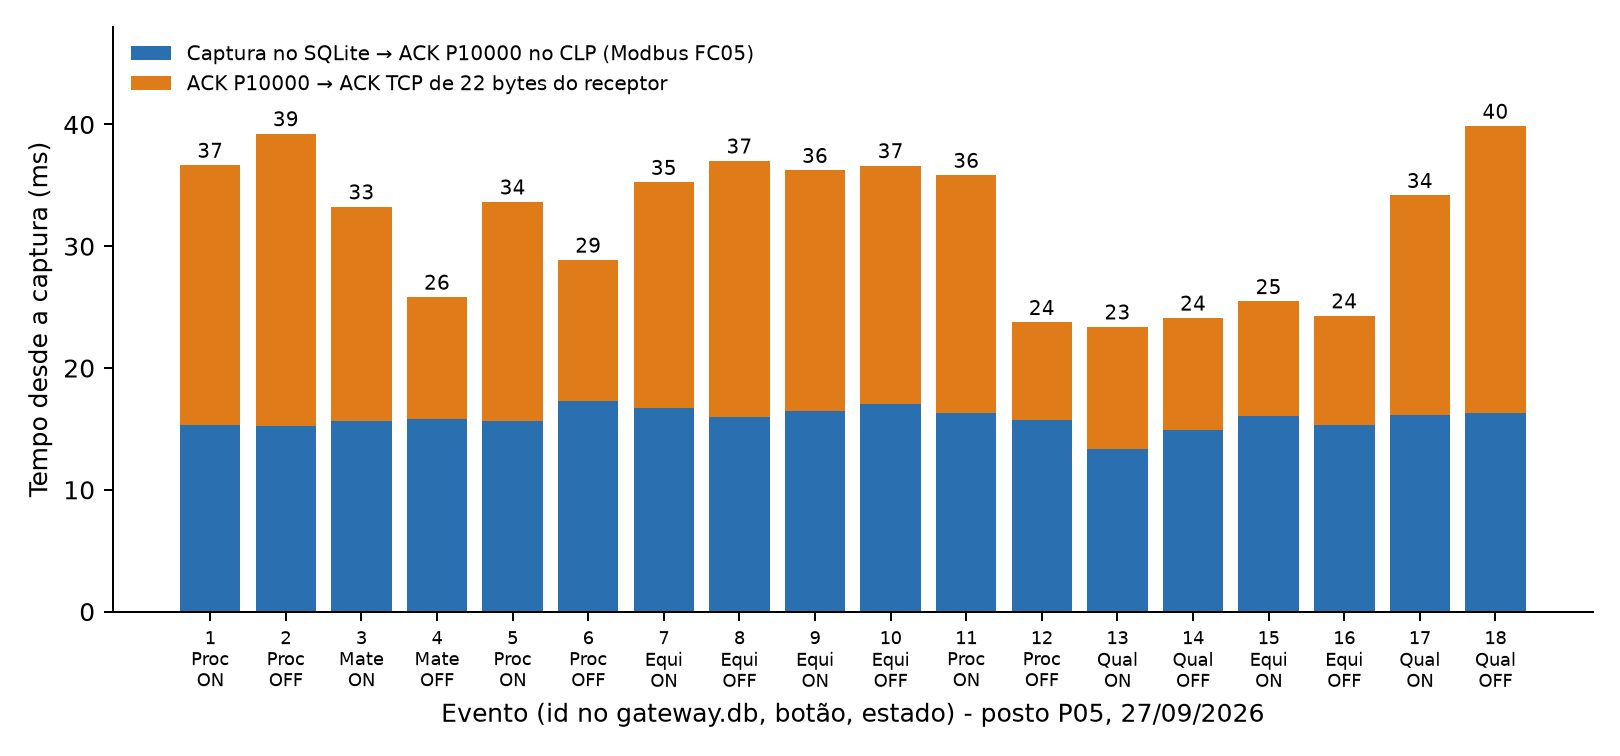
\includegraphics[width=1.00\textwidth]{Imagens/ev_latencia_eventos_reais.png}
    \caption{Latência dos 18 eventos reais (CLP LS XGK, 27/09/2026), calculada a partir de \cod{captured\_at}, \cod{plc\_acknowledged\_at} e \cod{confirmed\_at} de \cod{gateway.db}. (arquivo: Imagens/ev\_latencia\_eventos\_reais.png)}
    \label{fig:latencia}
\end{figure}

\textbf{Retenção na FIFO durante a perda de comunicação.} Às 20:48:23 o Gateway deixou de receber respostas do CLP e, em seguida, a porta COM10 desapareceu (adaptador desconectado). Os eventos 13 a 16 têm carimbo do CLP entre 22:19:09 e 22:19:56, ou seja, foram gerados enquanto o Gateway estava sem comunicação. Eles ficaram retidos na FIFO \cod{D00300} e foram capturados na reconexão, às 22:26:21,69, 22:26:21,91, 22:26:22,17 e 22:26:22,42 - um evento a cada ciclo de leitura de 250 ms, na ordem original e sem perda. A regra ``um evento por vez, liberado somente após \cod{P10000}'' do Ladder é o que garante esse comportamento.

\section{Raspberry Pi - Gateway de borda (item 2c)}

\subsection{Função e organização do software}

O Gateway é um serviço Python sem interface gráfica que roda na Raspberry Pi (Raspberry Pi OS, Linux ARM64) e faz a ponte entre a porta serial do CLP e a rede IP. Cada responsabilidade é executada em uma \textit{thread} própria, iniciada e encerrada pela classe \cod{GatewayApplication} (Tabela \ref{tab:gwmodulos}).

{\footnotesize
\begin{longtable}{|>{\raggedright\arraybackslash}p{3.6cm}|>{\raggedright\arraybackslash}p{11.0cm}|}
\caption{Módulos do pacote \cod{hardware/gateway/}.}\label{tab:gwmodulos}\\
\hline
\textbf{Módulo} & \textbf{Responsabilidade} \\ \hline
\endfirsthead
\hline
\textbf{Módulo} & \textbf{Responsabilidade} \\ \hline
\endhead
\cod{application.py} & Inicia e encerra os serviços na ordem correta; atende ao arquivo de parada (\cod{--stop-file}) e aos sinais do sistema. \\ \hline
\cod{plc\_poller.py} & Ciclo de leitura a cada 250 ms (\cod{D100}-\cod{D160}, \cod{D1200}, estados e contador); captura o evento, faz o COMMIT e só então liga \cod{P10000}; serializa todos os comandos na mesma \textit{thread} da porta serial. \\ \hline
\cod{modbus\_transport.py} & Cliente \cod{pymodbus} RTU: FC03, FC04, FC05, FC06 e FC16, com verificação de cada resposta e fechamento da porta em caso de erro. \\ \hline
\cod{register\_map.py} & Decodifica os 61 registradores: evento, Andons em \textit{nibbles}, comando do motor e tempos UInt32. \\ \hline
\cod{cycle\_control.py} & Gravação e conferência da base de tempos (12 blocos de 24 palavras), pulso de Start com confirmação em até 8 s e pulso de reset com conferência de \cod{D16052 = 0}. \\ \hline
\cod{persistence.py} & SQLite com \cod{WAL} e \cod{synchronous=FULL}; fila FIFO durável; identificador = Gateway + carimbo do pacote + CRC32, sempre comparando os 16 bytes. \\ \hline
\cod{tcp\_sender.py} & Envia um evento por vez ao receptor e só o confirma após o ACK de 22 bytes; nova tentativa com espera crescente. \\ \hline
\cod{opcua\_server.py} & Servidor OPC UA com 74 variáveis e 6 métodos (seção 8). \\ \hline
\cod{security.py} & Valida certificados de cliente: confiança explícita, validade, \cod{clientAuth} e \cod{ApplicationUri}. \\ \hline
\cod{ntp\_client.py}, \cod{plc\_clock.py} & Cliente SNTP (UDP 123) e codificação BCD das quatro palavras de \cod{DATEWR}. \\ \hline
\cod{motor\_output.py} & \textit{Thread} do DRV8825: rampa de aceleração e desaceleração, frequência proporcional a \cod{D1200} e desabilitação segura em falha. \\ \hline
\end{longtable}
}

\subsection{Instalação como serviço}

O pacote é copiado para a Raspberry e instalado com \cod{sudo bash deploy/install.sh <servidor> <porta-serial> <id>}. O instalador cria o usuário de serviço \cod{gateway} (grupo \cod{dialout}, que dá acesso à serial), instala o código em \cod{/opt/lean-gateway} com uma \cod{venv} própria, grava a configuração em \cod{/etc/lean-gateway/config.toml} (uma configuração existente nunca é sobrescrita) e habilita a unidade \cod{gateway.service} do systemd. A unidade reinicia o serviço em 3 s após qualquer falha (\cod{Restart=always}), depende de \cod{network-online.target} e \cod{pigpiod.service} e roda com \cod{ProtectSystem=strict}, \cod{ProtectHome=true} e \cod{NoNewPrivileges=true}; só pode escrever em \cod{/var/lib/lean-gateway} (banco) e \cod{/var/log/lean-gateway} (log). O guia \cod{hardware/README\_INSTALACAO\_RASPBERRY.md} detalha os 17 passos, da gravação do cartão SD ao diagnóstico.

\subsection{Motor da esteira (DRV8825)}

Com \cod{D112 = 1} e \cod{D1200 > 0}, a \textit{thread} do motor acelera até a frequência
\[
f = f_{min} + (f_{max} - f_{min}) \cdot \frac{D1200}{100}, \qquad f_{min} = 100\ \text{Hz},\ f_{max} = 5000\ \text{Hz},
\]
com \textit{duty cycle} de 50 \% no pino STEP (GPIO 18) e rampa de 0,5 s. \cod{D112 = 0} ou \cod{D1200 = 0} desaceleram até zero e desabilitam o driver (EN, GPIO 15, ativo em nível baixo, com \textit{pull-up} externo de 10 k$\Omega$). Falha de leitura ou valor inválido desabilitam EN imediatamente, sem rampa. O sentido é fixo (DIR, GPIO 25). Por exemplo, com \cod{D1200 = 60} a frequência comandada é $100 + 4900 \times 0{,}60 = 3040$ Hz.

\subsection{Relógio do CLP}

O cliente SNTP consulta o servidor central, valida modo, versão, \textit{stratum} e o carimbo de origem, converte a hora para \cod{America/Manaus} e grava \cod{D1000}-\cod{D1003} em uma única escrita FC16; em seguida liga \cod{P10001} e o Ladder executa \cod{DATEWRP}. Se o NTP não responder na partida, o Gateway aplica uma única vez a hora do próprio sistema e continua tentando o NTP. O serviço não altera o relógio da Raspberry.

\subsection{Evidência: execução real com o CLP}

O arquivo \cod{hardware/logs/gateway.log} registra a execução do Gateway \cod{LINHA\_A} com o CLP real entre 27/09/2026 16:57:51 e 28/09/2026 13:11:27 (Tabela \ref{tab:gwlog} e Figura \ref{fig:gwlog}).

{\footnotesize
\begin{longtable}{|>{\raggedright\arraybackslash}p{6.2cm}|>{\centering\arraybackslash}p{2.0cm}|>{\raggedright\arraybackslash}p{6.4cm}|}
\caption{Resumo do \cod{gateway.log} da execução real (32.140 linhas: 27.637 INFO, 7 WARNING e 4.466 ERROR).}\label{tab:gwlog}\\
\hline
\textbf{Registro} & \textbf{Ocorrências} & \textbf{Significado} \\ \hline
\endfirsthead
\hline
\textbf{Registro} & \textbf{Ocorrências} & \textbf{Significado} \\ \hline
\endhead
\cod{Gateway LINHA\_A started} & 4 & Partidas do serviço (27/09 16:57 e três em 28/09 entre 13:08 e 13:11). \\ \hline
\cod{Modbus: connected} & 4 & Comunicação estabelecida com o CLP na COM10. \\ \hline
\cod{OPC UA: active and secure} & 4 & Servidor OPC UA ativo com \cod{Basic256Sha256}. \\ \hline
\cod{SNTP: synchronized} & 2 & 16:57:51 e 22:26:23 (logo após a reconexão Modbus). \\ \hline
\cod{TCP: event N confirmed} & 18 & Eventos 1 a 18 entregues ao receptor, em ordem. \\ \hline
\cod{Modbus: unavailable} & 9 & Perda de resposta do CLP ou da porta serial. \\ \hline
\cod{could not open port 'COM10'} (pymodbus, ERROR) & 4.444 & Tentativas de reabrir a porta a cada 2 s enquanto o adaptador estava desconectado. \\ \hline
\cod{SNTP: network time could not be applied} & 591 & O SNTP obteve a hora, mas não conseguiu gravá-la no CLP; tentou de novo a cada 10 s. \\ \hline
\cod{Stop file received} ... \cod{Gateway stopped} & 1 & Encerramento ordenado em 28/09 13:11:25: SNTP, OPC UA, Modbus, TCP e SQLite. \\ \hline
\end{longtable}
}

\begin{figure}[H]
    \centering
    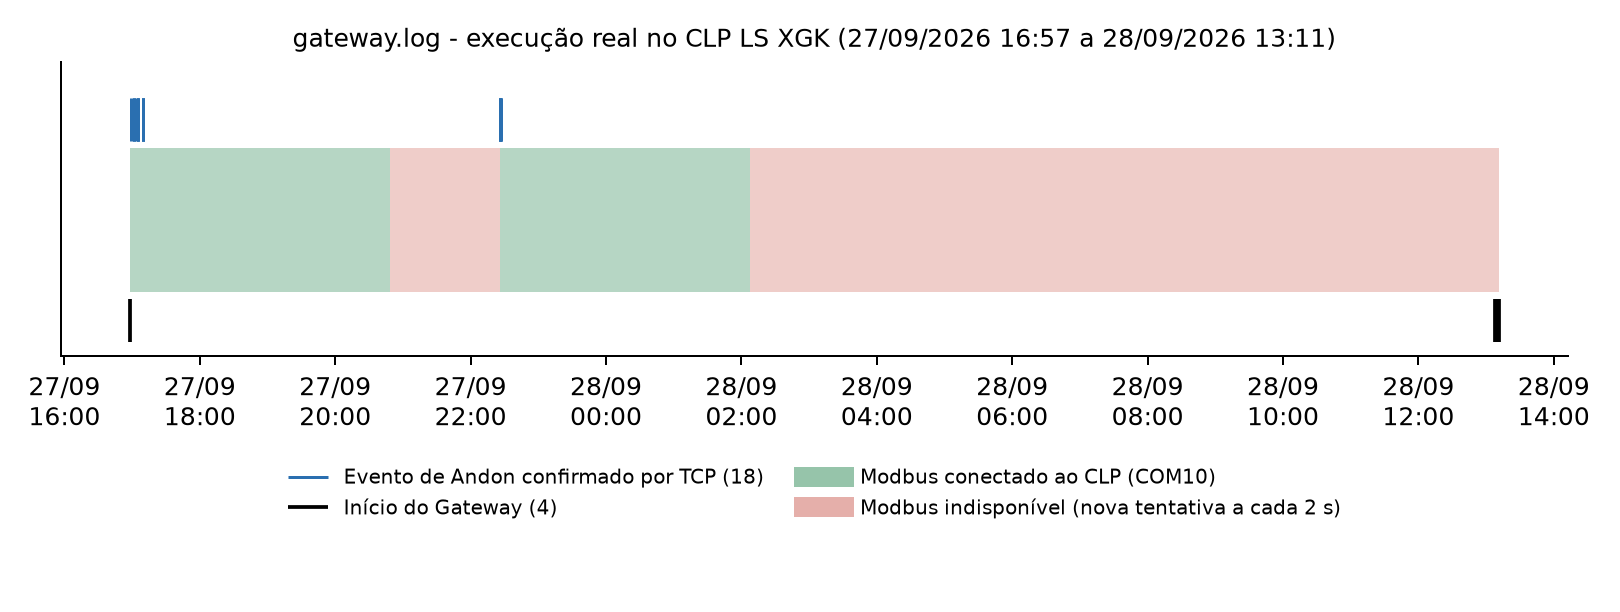
\includegraphics[width=1.00\textwidth]{Imagens/ev_linha_tempo_gateway_log.png}
    \caption{Linha do tempo da execução real: períodos com Modbus conectado (verde) e indisponível (vermelho), eventos confirmados e partidas do serviço. (arquivo: Imagens/ev\_linha\_tempo\_gateway\_log.png)}
    \label{fig:gwlog}
\end{figure}

A Figura \ref{fig:gwlog} mostra dois períodos de comunicação. O primeiro (16:57 a 20:48) concentra os eventos 1 a 12. Após a perda de comunicação de 20:48, o serviço não encerrou: manteve o OPC UA e o TCP ativos, tentou reabrir a porta a cada 2 s e, quando o adaptador voltou (22:26:21), retomou a leitura, entregou os quatro eventos retidos na FIFO do CLP (seção 3.5), sincronizou o relógio dois segundos depois e capturou os eventos 17 e 18. A segunda interrupção (02:07) não foi seguida de reconexão até o encerramento manual. Os 4.444 erros \cod{could not open port} são, portanto, a evidência do mecanismo de reconexão, e não falhas de processamento: nenhum evento foi perdido ou duplicado (18 capturados, 18 confirmados, \cod{attempts = 0}).

\subsection{Evidência: Gateway real contra o CLP emulado}\label{sec:emulado}

Para demonstrar os comandos de base, Start e reset e para capturar telas sem o hardware, o Gateway foi executado sem nenhuma alteração de código contra \cod{clp\_emulado.py}, um servidor Modbus RTU (biblioteca pymodbus) que expõe o mesmo mapa da Tabela \ref{tab:mapa} e imita o Ladder de forma simplificada: fila de eventos com o \textit{handshake} \cod{D100}/\cod{P10000}, aplicação do relógio por \cod{P10001}, base de tempos em \cod{D17001}, Start por \cod{P10002}, reset por \cod{P10003}, fluxo de uma peça por vez entre os 12 postos com os estados 0 a 3, contador \cod{D16052}, Andons em \cod{D109}-\cod{D111} e comando do motor em \cod{D112}. O Gateway apenas troca a porta serial por \cod{socket://127.0.0.1:5020}, recurso da própria pyserial; o protocolo continua sendo Modbus RTU, com CRC.

Na execução de 21/11/2026 (20:13 a 20:18), o Gateway \cod{LINHA\_DEMO}:
\begin{itemize}
    \item conectou-se, habilitou a leitura dos estados e do contador (\cod{process status available}, \cod{production count available}) e, sem servidor NTP disponível, aplicou a hora do sistema ao CLP uma única vez. O CLP emulado recebeu \cod{D1000}-\cod{D1003} = \cod{0x1126 0x2021 0x5313 0x2006}, isto é, 21/11/(20)26, 20:13:53, sábado (6) - codificação BCD correta;
    \item gravou e conferiu as 288 palavras da base (\cod{POST /api/process/cycle-base}, 5,3 s), pulsou \cod{P10002} e confirmou o Start quando o P01 chegou ao estado 2 (\cod{confirmed: true});
    \item capturou e entregou 6 eventos de Andon (P05 Equipamento, P09 Qualidade e P03 Material, ligado e desligado), com ACK no CLP entre 15,1 e 17,3 ms (mediana 15,9 ms) e entrega TCP entre 21,3 e 46,4 ms (mediana 23,1 ms), valores da mesma ordem dos medidos com o CLP real;
    \item executou o reset (\cod{P10003}, 2,7 s) e conferiu \cod{D16052 = 0}, e encerrou de forma ordenada pelo arquivo de parada.
\end{itemize}

\section{Desktop - Simulador da Linha (item 2a)}

\subsection{Função}

O Desktop (\cod{simulador/main.py}, iniciado por \cod{run\_mock.ps1}) é um aplicativo PyQt6 que substitui o CLP e o Gateway quando o hardware não está disponível, falando os mesmos protocolos: envia cada Andon pelo protocolo binário de 16 bytes ao receptor (TCP 15000) e publica a telemetria no mesmo servidor OPC UA seguro, com os mesmos 72 NodeIds do Gateway. Dessa forma, o receptor e a Dashboard funcionam sem alteração com o simulador ou com a linha real. A janela (Figura \ref{fig:desk1}) mostra, para os postos 01 a 12, os quatro Andons (Qualidade, Equipamento, Processo e Material) e os campos de Takt time e último ciclo; o rodapé informa o estado do TCP e a fila (pendentes e confirmados), e o cabeçalho, o estado do OPC UA.

\begin{figure}[H]
    \centering
    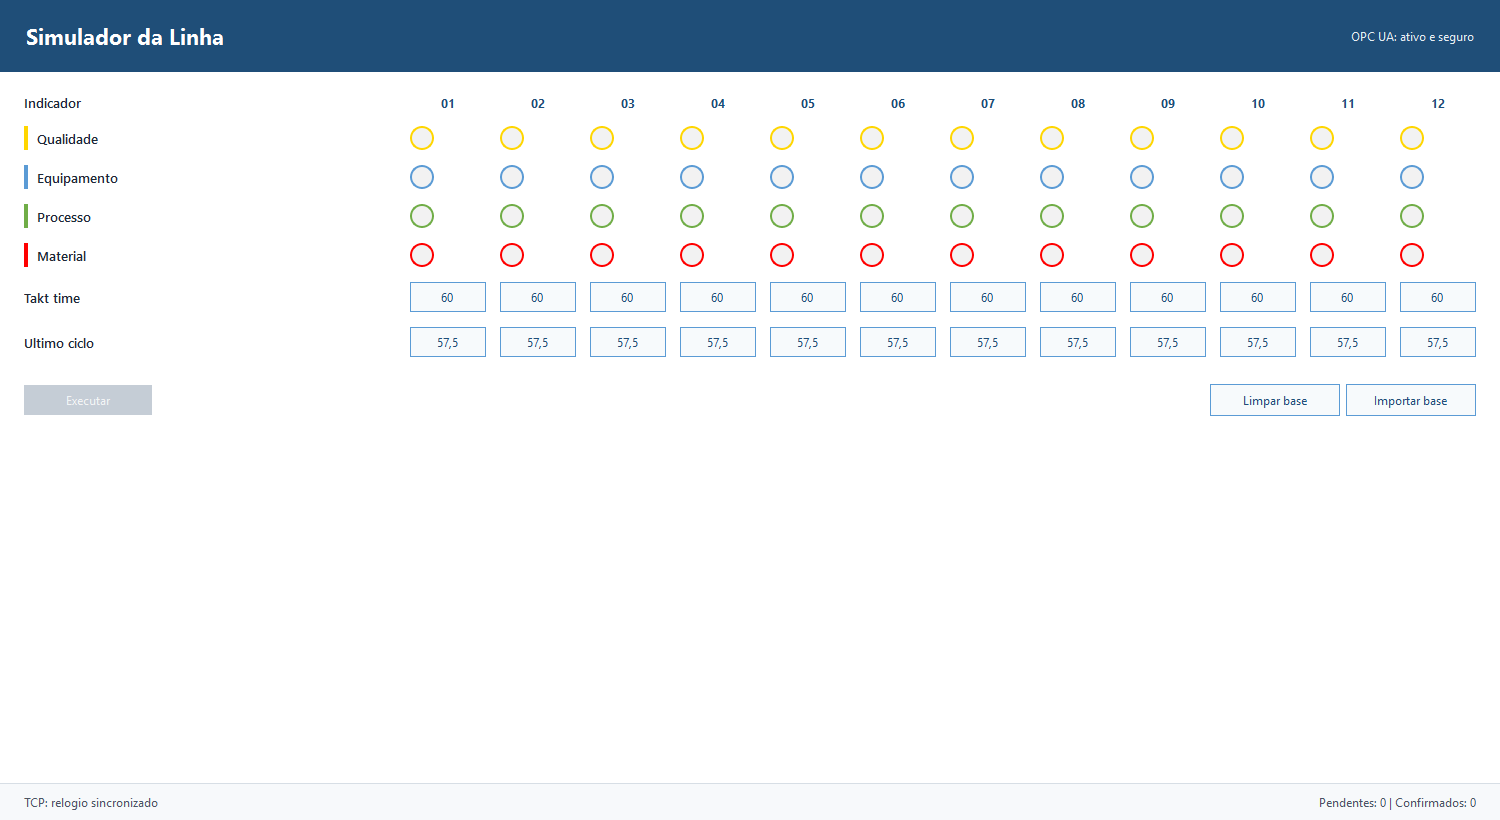
\includegraphics[width=1.00\textwidth]{Imagens/desk_01_inicial.png}
    \caption{Janela do Simulador da Linha ao iniciar: 48 Andons desligados, Takt 60 s e último ciclo 57,5 s (valores de \cod{config.toml}), OPC UA ``ativo e seguro''. (arquivo: Imagens/desk\_01\_inicial.png)}
    \label{fig:desk1}
\end{figure}

\subsection{Regras de funcionamento}

\begin{itemize}
    \item Um clique registra uma única data e hora lógica, alterna somente o botão escolhido e, na mesma transação SQLite, grava o novo estado e o pacote imutável de 16 bytes. A interface só muda depois do COMMIT; se o banco falhar, o estado visual não muda e uma mensagem de erro é exibida.
    \item A fila de saída é global e estritamente FIFO pelo identificador autoincremental. Apenas um evento fica em trânsito; o seguinte espera o ACK válido do anterior. Falhas usam esperas de 1, 2, 5, 10 e 30 s, permanecendo em 30 s; ao reiniciar, os estados são restaurados e o primeiro evento pendente é retomado.
    \item As quatro categorias de um posto são independentes e podem ficar ligadas ao mesmo tempo (\cod{test\_multiple\_categories\_can\_be\_on}); cada mudança gera um evento próprio.
    \item Takt time e último ciclo podem ser editados por posto e são publicados no OPC UA pelo botão \textbf{Executar}. \textbf{Importar base} reproduz planilhas \cod{.xlsx}, \cod{.xlsm} ou \cod{.csv} publicando um par Takt/ciclo por segundo; 26 planilhas de exemplo estão em \cod{bases\_exemplo/} (operação estável, gargalo fixo no P06, gargalo migrando, linha balanceada e desbalanceada, entre outras).
    \item Com \cod{sync\_on\_start = true}, o Desktop pede a hora ao receptor (pacote \cod{00 01} seguido de 14 bytes zero) e passa a usar um relógio lógico monotônico, sem alterar o relógio do Windows.
\end{itemize}

\subsection{Evidência: Desktop $\rightarrow$ receptor $\rightarrow$ Dashboard}

Em 21/11/2026 o Desktop foi executado com um receptor dedicado (portas 4851, 8092 e 15011). Na partida, o Desktop sincronizou o relógio (\cod{HORA respondida} às 20:24:45) e o cliente OPC UA do receptor conectou-se ao servidor do simulador. Foi acionado o Andon de Material do P03 e, 18 s depois, liberado (Figuras \ref{fig:desk2} e \ref{fig:desk3}). O terminal do receptor registrou:

{\scriptsize
\begin{verbatim}
[2026-11-21T20:24:51.208851-04:00] posto=03 botao=Material estado=ON resultado=ON ACK=enviado
[2026-11-21T20:25:09.694850-04:00] posto=03 botao=Material estado=OFF resultado=OFF ACK=enviado
\end{verbatim}
}

O banco do Desktop (\cod{outbox\_event}) registra os dois pacotes, \cod{00 01 00 03 11 26 20 21 50 24 20 06 00 04 00 01} (ON) e \cod{... 00 04 00 02} (OFF), ambos com \cod{delivery\_status = confirmed}, \cod{attempts = 0} e 11,5 ms e 10,5 ms entre a gravação na fila e o ACK do receptor. Na base histórica do simulador (\cod{simulador/data/mock\_line.db}) os quatro eventos gerados em 21/11/2026 entre 20:01 e 20:02 foram confirmados entre 10,5 e 14,5 ms.

\begin{figure}[H]
    \centering
    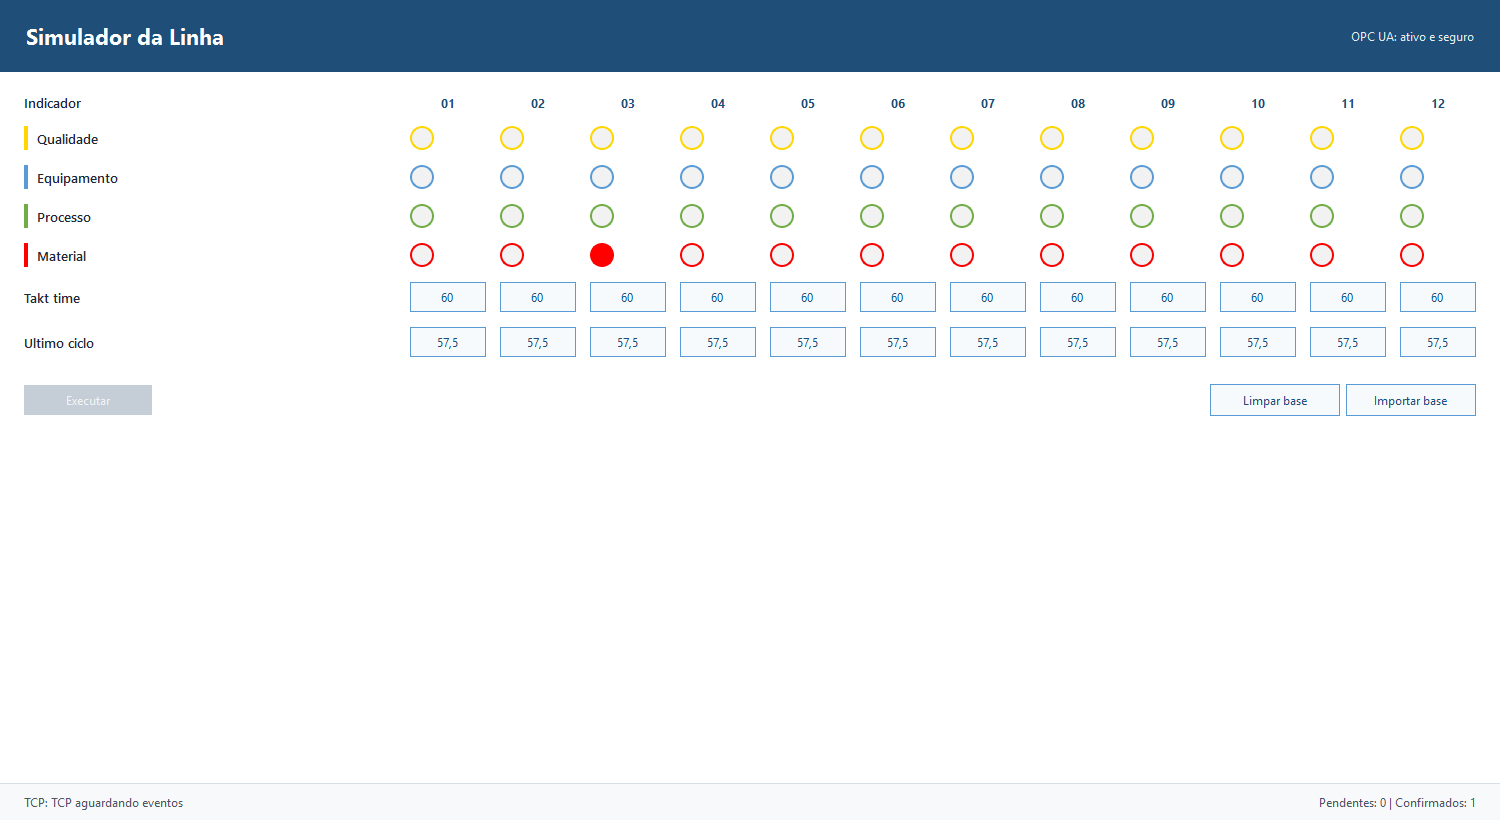
\includegraphics[width=1.00\textwidth]{Imagens/desk_02_andon_ativo.png}
    \caption{Andon de Material do posto 03 aceso; rodapé ``Pendentes: 0 | Confirmados: 1'' (o evento ON já recebeu o ACK). (arquivo: Imagens/desk\_02\_andon\_ativo.png)}
    \label{fig:desk2}
\end{figure}

\begin{figure}[H]
    \centering
    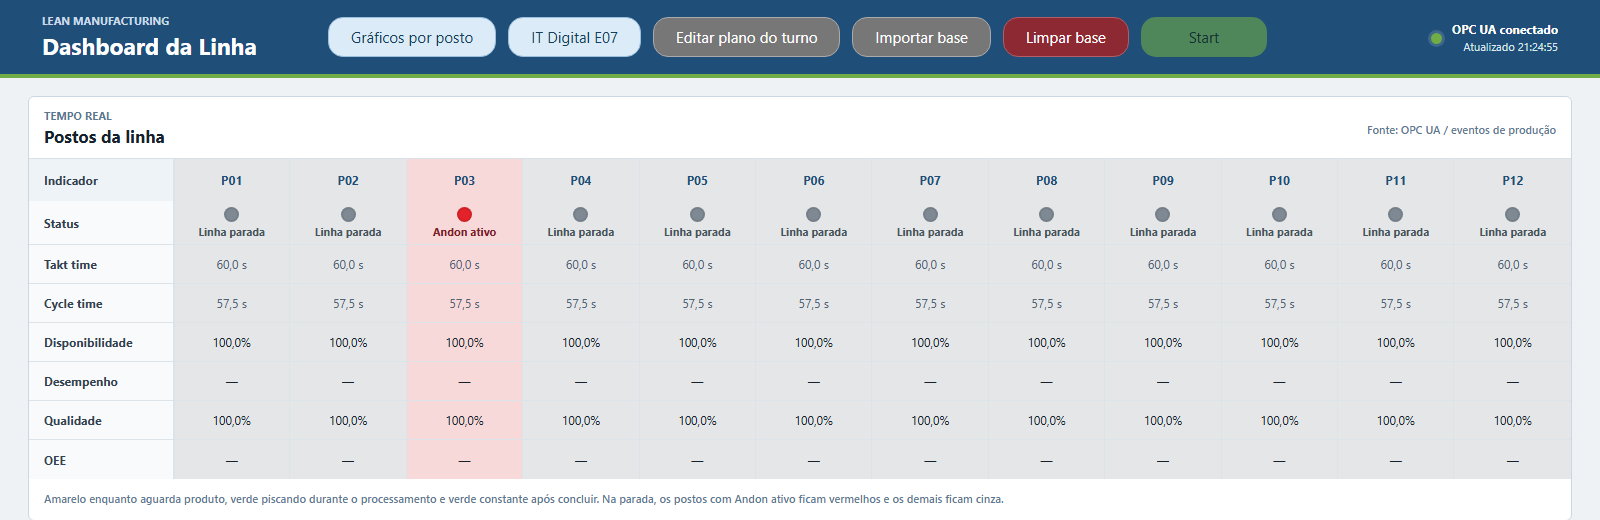
\includegraphics[width=1.00\textwidth]{Imagens/desk_04_dashboard_simulador.png}
    \caption{Dashboard alimentada pelo Desktop no mesmo instante: coluna P03 em vermelho (``Andon ativo'') e os demais postos em ``Linha parada''. (arquivo: Imagens/desk\_04\_dashboard\_simulador.png)}
    \label{fig:desk3}
\end{figure}

Os testes automatizados do Desktop (Tabela \ref{tab:testes}, seção 9) cobrem a atomicidade do clique (\cod{test\_toggle\_is\_atomic\_and\_persists\_queue}), o \textit{rollback} em falha de codificação, a restauração após reinício, a fila FIFO com reenvio (\cod{test\_sender\_retries\_head\_then\_preserves\_fifo}), a janela com 12 postos e a publicação da planilha importada com intervalo de 1 s.

\section{Dashboard web (item 2b)}

\subsection{Função e telas}

A Dashboard é servida pelo receptor (\cod{run\_receiver.ps1}, módulo \cod{simulador/web/dashboard.py}, FastAPI + uvicorn) na porta 8081 e é atualizada a cada 1 s pelo WebSocket \cod{/ws}. O indicador ``OPC UA conectado'' no cabeçalho é verde quando a última notificação do Gateway tem menos de 10 s (\cod{opcua\_stale\_seconds}). A página principal tem três blocos:

\begin{itemize}
    \item \textbf{Postos da linha} - uma coluna por posto com status, Takt time, Cycle time (último ciclo), Disponibilidade, Desempenho, Qualidade e OEE. A cor da coluna segue o estado \cod{D01651}-\cod{D01662}: amarelo nos estados 0 e 1 (aguardando), verde piscando no 2 (processando) e verde constante no 3 (finalizou). Com um Andon ativo, a coluna do posto fica vermelha e as demais cinza (``Linha parada'').
    \item \textbf{Plano e acompanhamento} - meta de produção e tempo disponível (editáveis em \textbf{Editar plano do turno}), tempo decorrido, tempo real de produção, produção estimada, produção atual (contador \cod{D16052}) e defeitos.
    \item \textbf{OEE da linha e Parada da linha} - os três fatores, o OEE consolidado e os minutos parados por categoria de Andon.
\end{itemize}

A página \cod{/graficos} mostra o último ciclo (ou o Takt) de cada posto em barras, e o botão \textbf{IT Digital E07} abre a instrução de trabalho (seção 7). \textbf{Importar base}, \textbf{Start} e \textbf{Limpar base} acionam o CLP pelo caminho da Tabela \ref{tab:comandos}; o Start só é habilitado com a base conferida, os 12 postos no estado 0 e nenhum Andon ativo.

\subsection{Indicadores calculados}

Os cálculos estão em \cod{services/analytics.py} (revisão \cod{2026-11-20.01}, publicada em \cod{/api/version}). O período de medição começa no Start confirmado pelo CLP (ou no último reset) e termina no instante atual. Sendo $T$ o tempo decorrido, $S$ o tempo parado, $M$ a meta do turno, $T_d$ o tempo disponível, $B$ as peças boas (contador do P12) e $D$ os defeitos:

\begin{align*}
\text{Produção esperada} &= M \cdot \frac{T}{60\,T_d} \\
\text{Produção estimada} &= \lfloor \text{Produção esperada} \rfloor \\
\text{Disponibilidade} &= 100 \cdot \frac{T - S}{T} \\
\text{Desempenho} &= 100 \cdot \frac{B}{\text{Produção estimada}} \\
\text{Qualidade} &= 100 \cdot \frac{B}{B + D} \\
\text{OEE} &= \frac{\text{Disponibilidade} \cdot \text{Desempenho} \cdot \text{Qualidade}}{10^4}
\end{align*}

O tempo parado $S$ é a \textbf{união} dos intervalos de todos os Andons (intervalos sobrepostos não são somados duas vezes); os minutos por categoria são calculados separadamente e a sobreposição é informada à parte. Um Andon de Qualidade ligado registra um defeito no posto. O Desempenho só é exibido quando há ao menos uma peça boa e uma peça estimada.

\subsection{Evidência: execução com o Gateway real e o CLP emulado}

A demonstração da seção \ref{sec:emulado} foi acompanhada pela Dashboard. O plano foi definido por \cod{PUT /api/process/production-plan} com meta de 90 peças em 60 min (Takt de 40 s) e a base \cod{base\_demo.csv} foi importada (P07 com ciclo de 36 s, demais postos entre 6 e 12 s). As Figuras \ref{fig:dash1} a \ref{fig:dash5} são capturas da página real, sem edição além do corte da área vazia.

\begin{figure}[H]
    \centering
    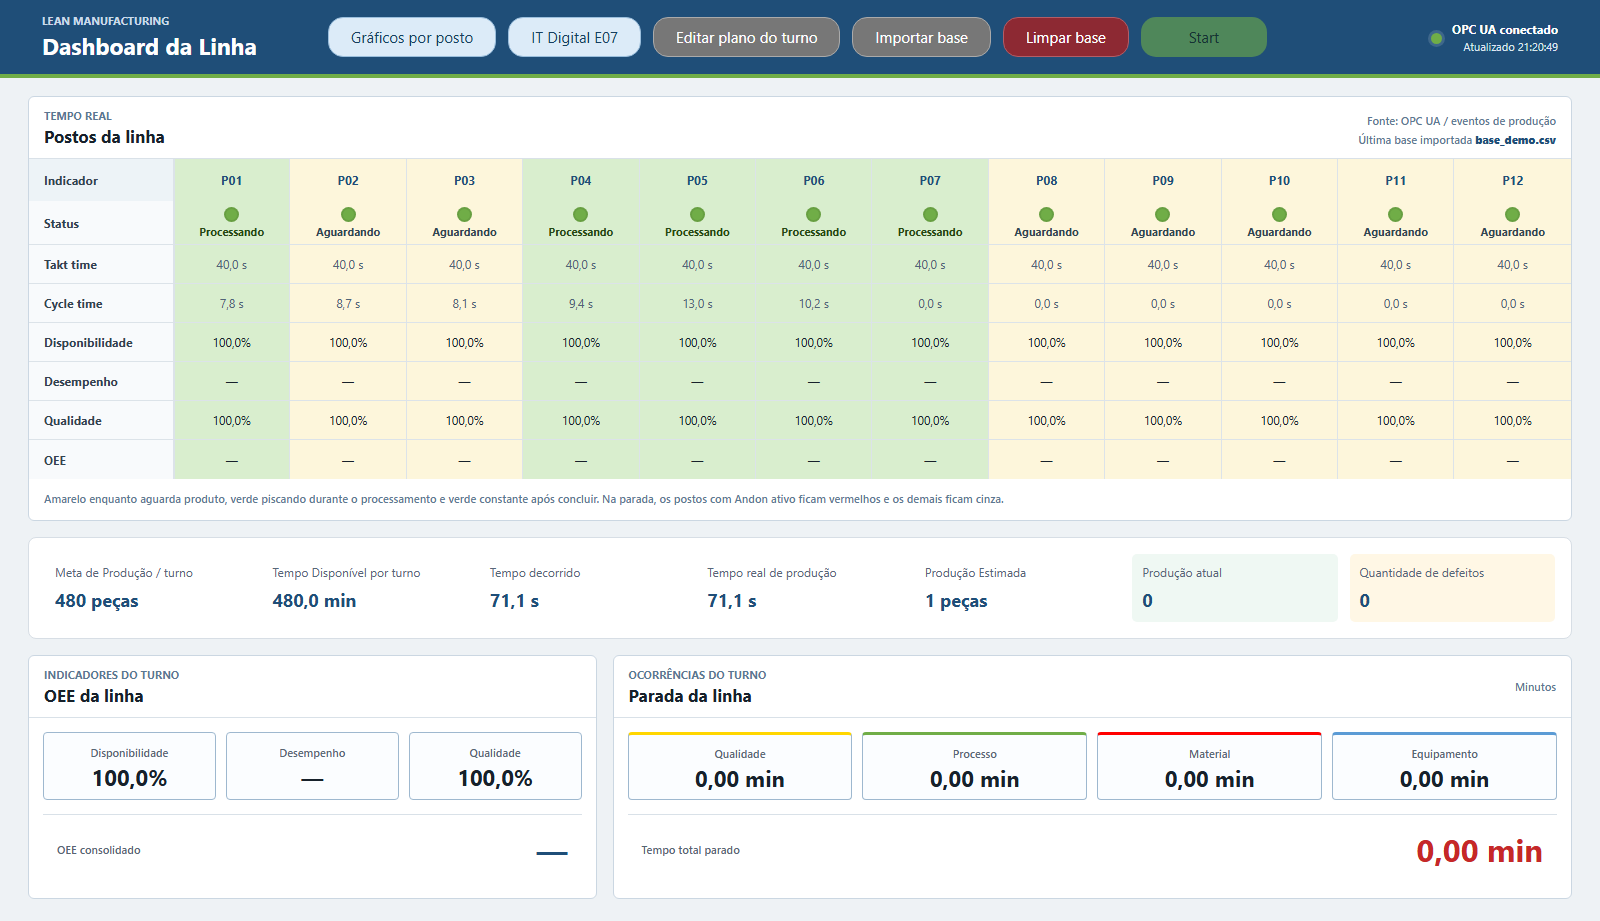
\includegraphics[width=1.00\textwidth]{Imagens/dash_06_p07_processando.png}
    \caption{Linha em operação: P01 e P04 a P07 processando (verde), demais aguardando (amarelo); nenhuma parada. (arquivo: Imagens/dash\_06\_p07\_processando.png)}
    \label{fig:dash1}
\end{figure}

\begin{figure}[H]
    \centering
    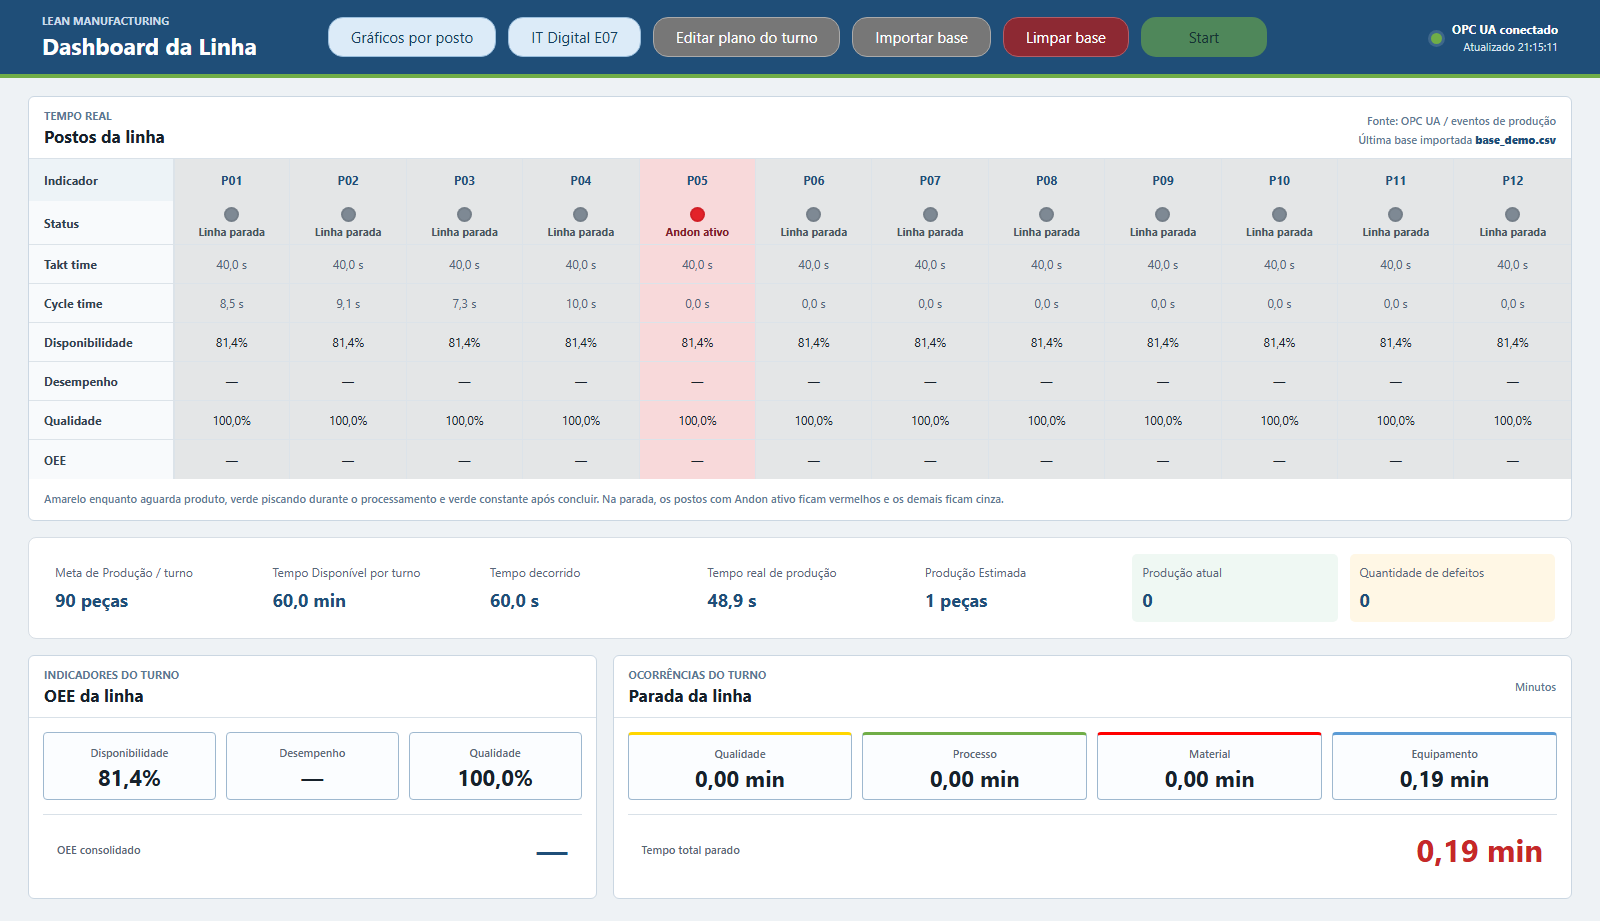
\includegraphics[width=1.00\textwidth]{Imagens/dash_02_andon_p05.png}
    \caption{Andon de Equipamento no P05, 50 s após o Start: coluna P05 vermelha, demais em ``Linha parada''; disponibilidade caindo (81,4 \%) e 0,19 min de parada por Equipamento. (arquivo: Imagens/dash\_02\_andon\_p05.png)}
    \label{fig:dash2}
\end{figure}

\begin{figure}[H]
    \centering
    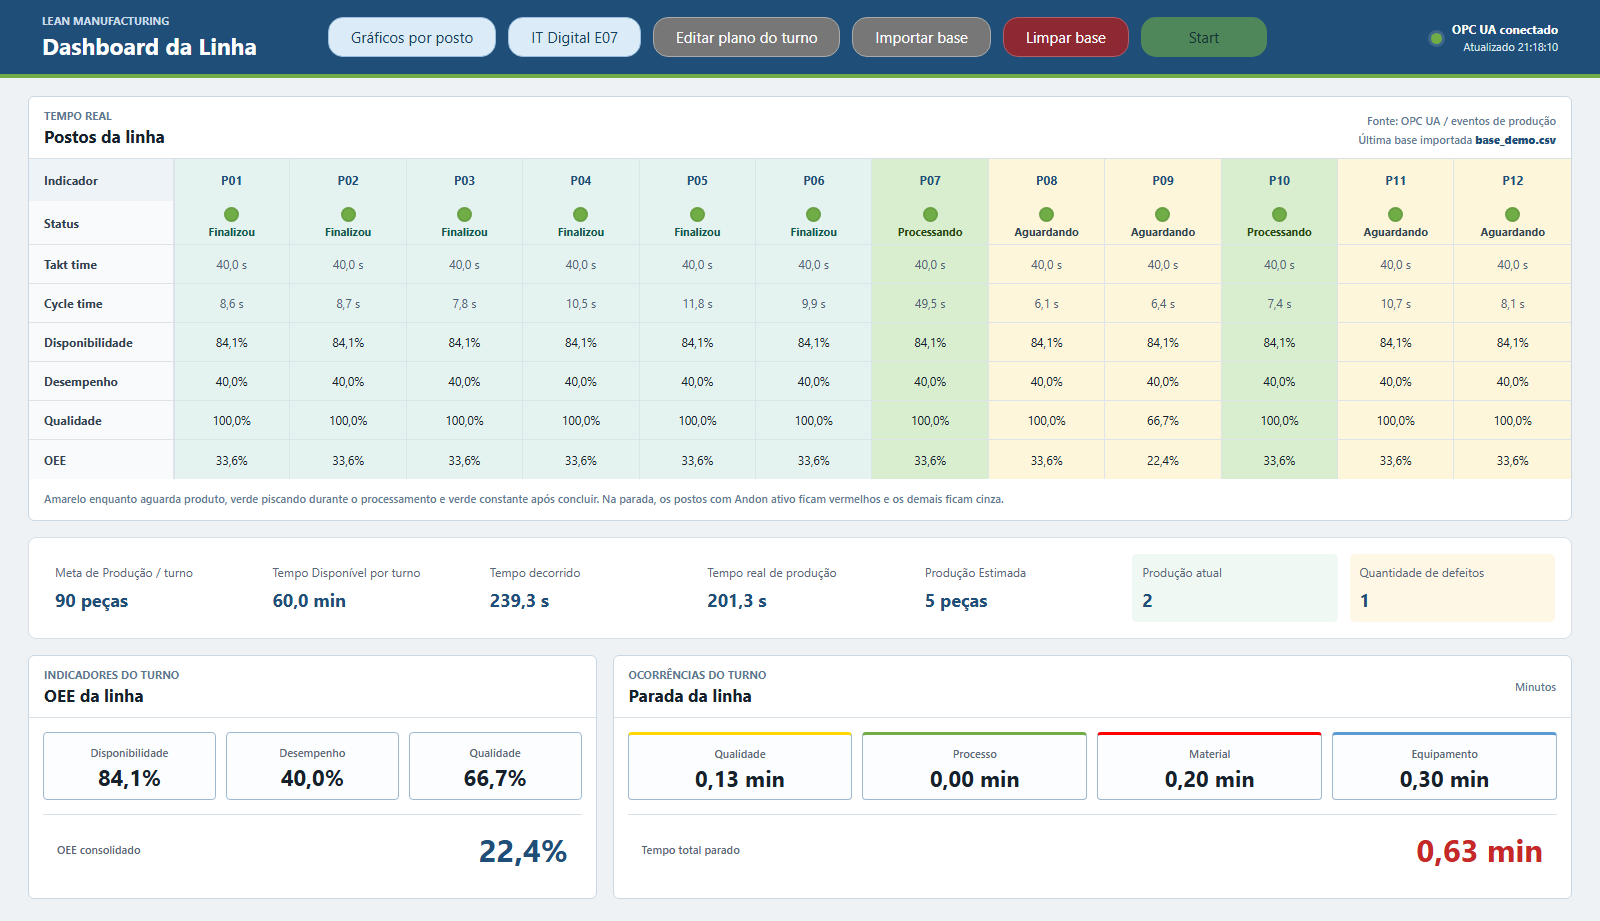
\includegraphics[width=1.00\textwidth]{Imagens/dash_03_final.png}
    \caption{Situação após 239,3 s: 2 peças produzidas, 1 defeito (Andon de Qualidade no P09), 0,63 min parados (Qualidade 0,13, Material 0,20 e Equipamento 0,30) e OEE de 22,4 \%. (arquivo: Imagens/dash\_03\_final.png)}
    \label{fig:dash3}
\end{figure}

\textbf{Conferência numérica da Figura \ref{fig:dash3}.} Com $T = 239{,}3$ s e $S = 38{,}0$ s (0,13 + 0,20 + 0,30 = 0,63 min, sem sobreposição), a Disponibilidade é $100 \cdot (239{,}3 - 38{,}0) / 239{,}3 = 84{,}1$ \%. A produção esperada é $90 \cdot 239{,}3 / 3600 = 5{,}98$, logo a estimada é 5 peças e o Desempenho é $100 \cdot 2/5 = 40{,}0$ \%. A Qualidade é $100 \cdot 2/(2+1) = 66{,}7$ \% na linha e no P09; nos demais postos, sem defeito, é 100 \%. O OEE é $84{,}1 \times 40{,}0 \times 66{,}7 / 10^4 = 22{,}4$ \% na linha e no P09 e $84{,}1 \times 40{,}0 \times 100 / 10^4 = 33{,}6$ \% nos demais postos - exatamente os valores exibidos.

\begin{figure}[H]
    \centering
    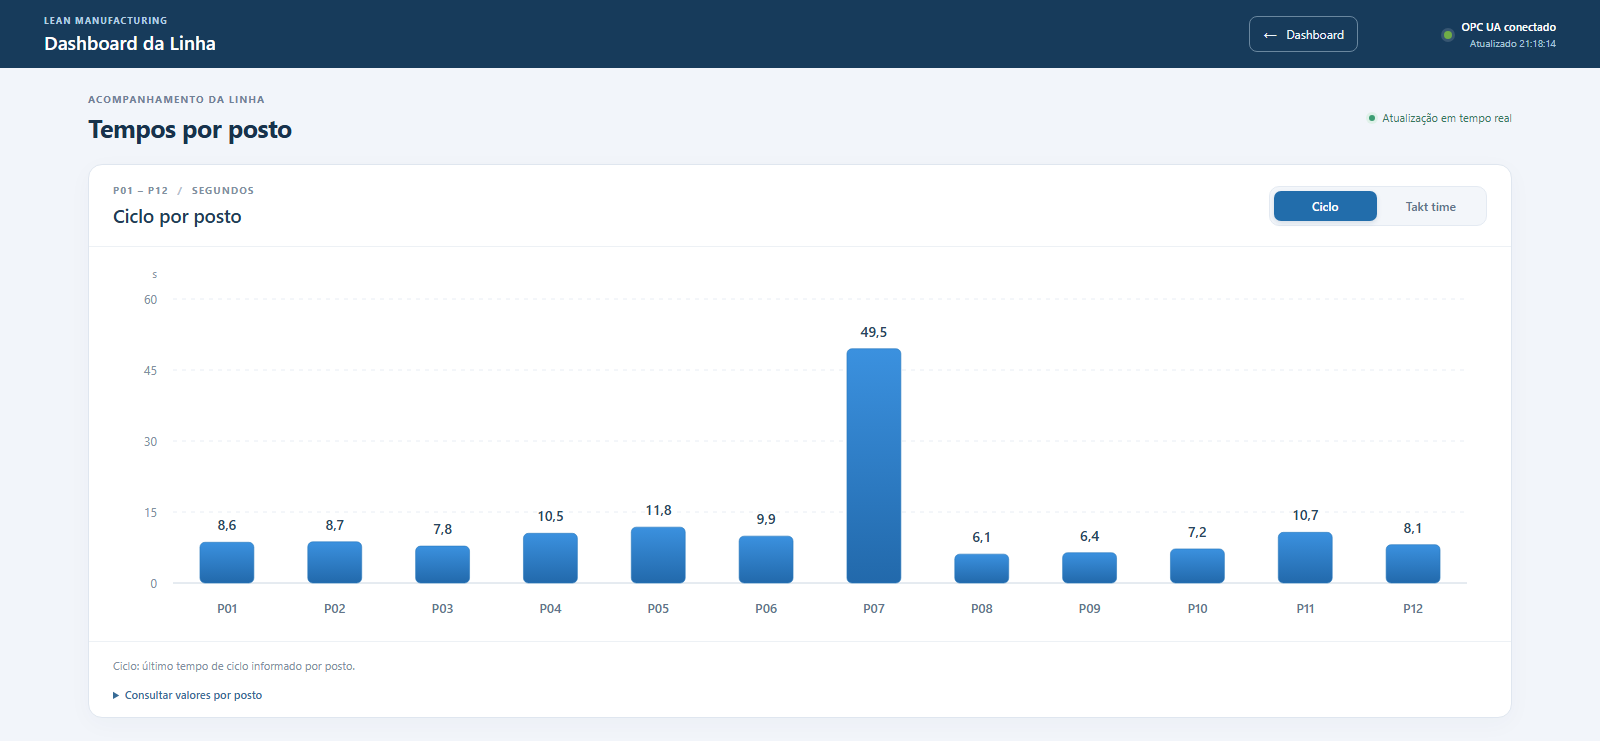
\includegraphics[width=1.00\textwidth]{Imagens/dash_04_graficos.png}
    \caption{Página \cod{/graficos}: último ciclo por posto. O P07 (49,5 s, contra Takt de 40 s) é o gargalo; o ciclo medido inclui o tempo em que o posto ficou parado pelos Andons. (arquivo: Imagens/dash\_04\_graficos.png)}
    \label{fig:dash4}
\end{figure}

\begin{figure}[H]
    \centering
    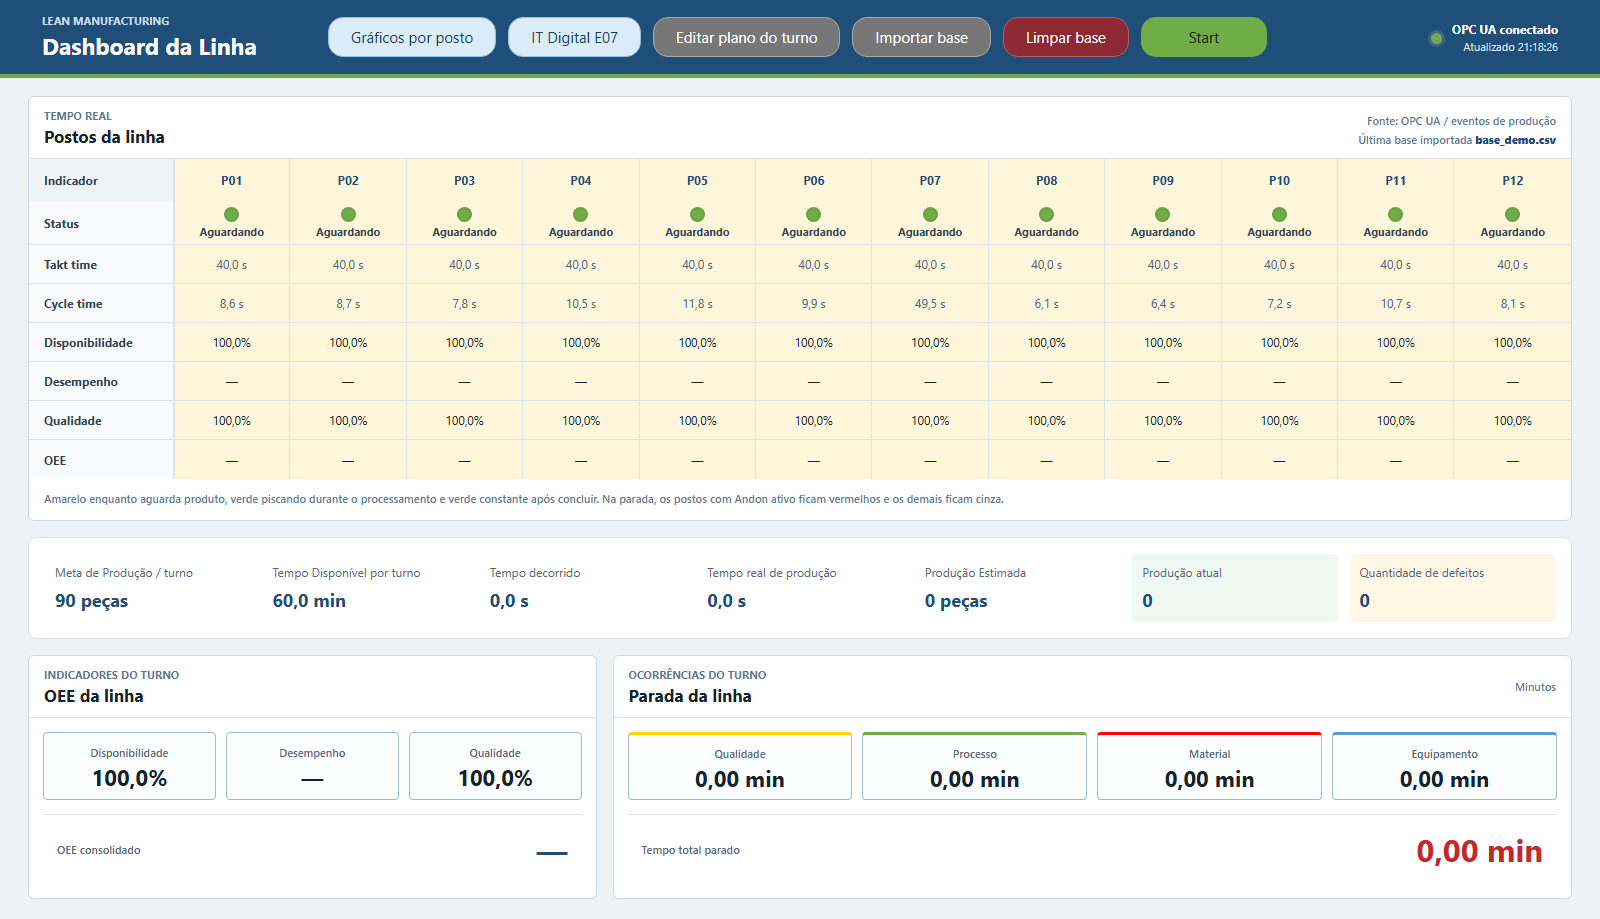
\includegraphics[width=1.00\textwidth]{Imagens/dash_05_apos_limpar.png}
    \caption{Após \textbf{Limpar base} (\cod{P10003} e \cod{D16052 = 0} conferidos): 12 postos aguardando, produção, defeitos e paradas do dia zerados e Start novamente habilitado. (arquivo: Imagens/dash\_05\_apos\_limpar.png)}
    \label{fig:dash5}
\end{figure}

A Figura \ref{fig:estados} reconstrói, a partir de 90 amostras de \cod{/api/snapshot}, os estados que a Dashboard recebeu para cada posto. Vê-se a primeira peça percorrer os postos em sequência, a fila que se forma antes do P07 (P01 a P06 em ``concluído'', aguardando a liberação do posto seguinte) e as paradas provocadas pelos Andons. A Figura \ref{fig:oee} mostra a produção atual acompanhando a estimada e a queda da disponibilidade a cada parada.

\begin{figure}[H]
    \centering
    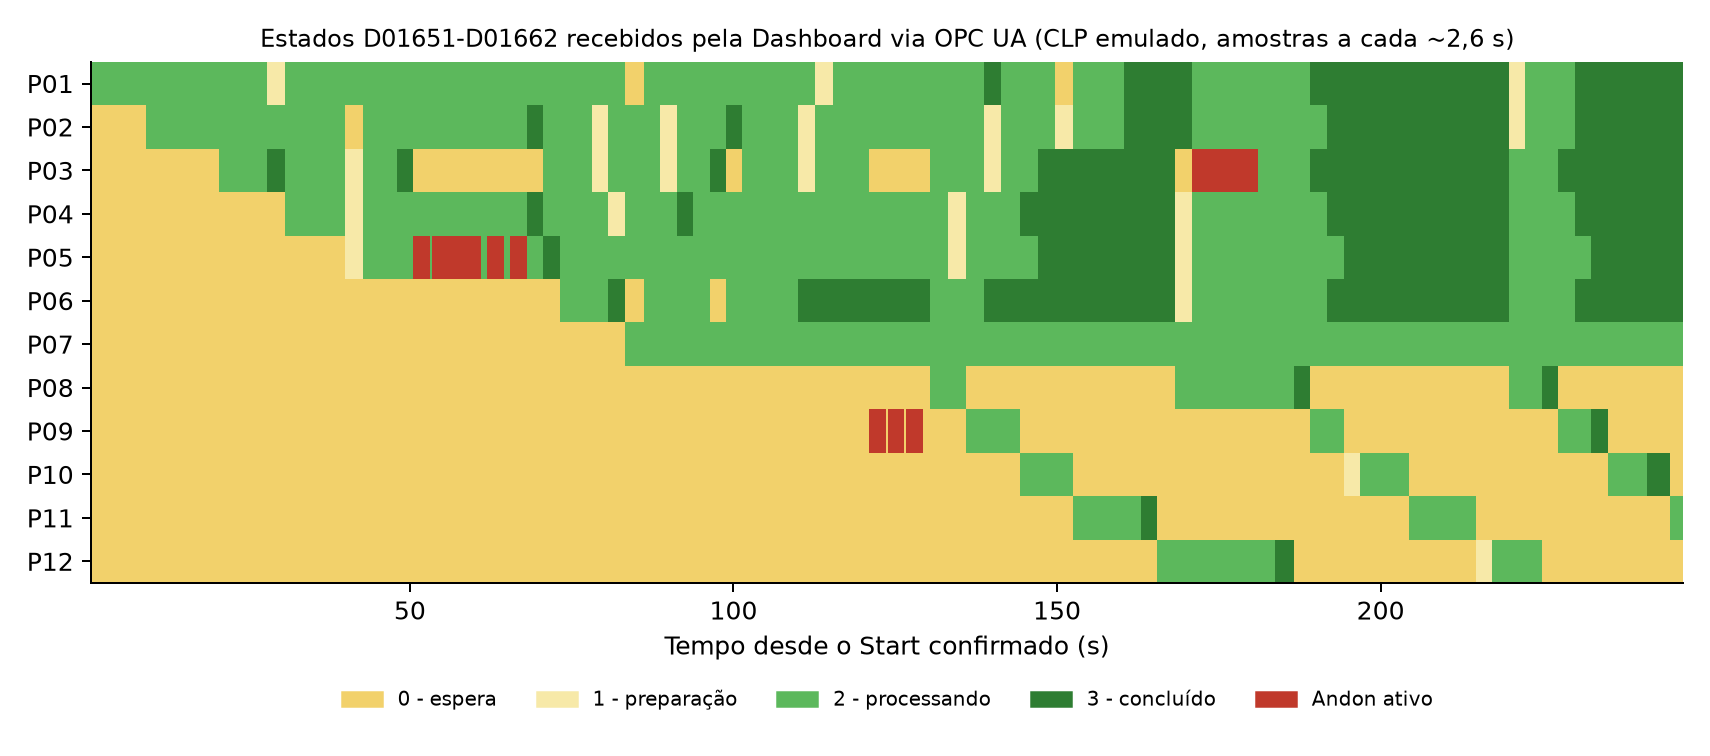
\includegraphics[width=1.00\textwidth]{Imagens/demo_estados_postos.png}
    \caption{Estados dos 12 postos recebidos pela Dashboard durante a demonstração (CLP emulado). (arquivo: Imagens/demo\_estados\_postos.png)}
    \label{fig:estados}
\end{figure}

\begin{figure}[H]
    \centering
    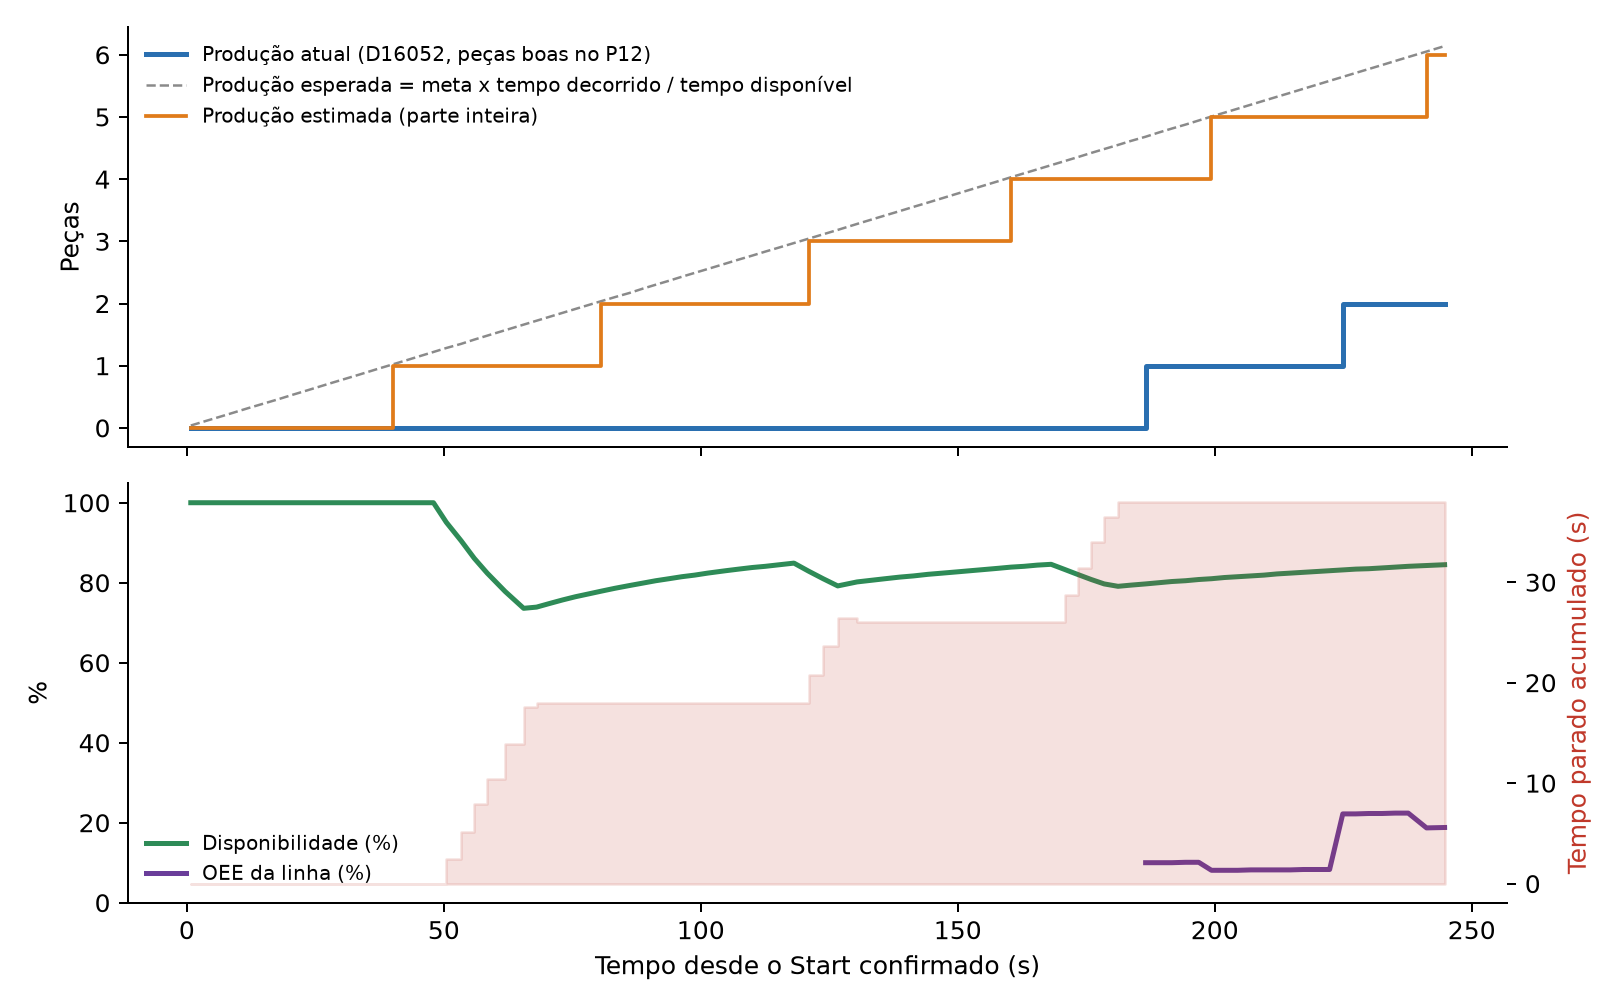
\includegraphics[width=0.95\textwidth]{Imagens/demo_producao_oee.png}
    \caption{Produção atual, esperada e estimada (acima); disponibilidade, OEE e tempo parado acumulado (abaixo), conforme \cod{/api/snapshot}. (arquivo: Imagens/demo\_producao\_oee.png)}
    \label{fig:oee}
\end{figure}

\subsection{Evidência: dados reais do receptor}

O banco do receptor da instalação (\cod{simulador/data/reference\_receiver.db}) contém 127 recepções de eventos (64 ON e 63 OFF, todas do tipo \cod{00 01}) entre 27/09/2026 e 21/11/2026: 18 em 27/09 (os eventos reais do CLP da seção 3.5), 4 em 30/09, 101 em 20/11 e 4 em 21/11. Delas resultaram 64 ocorrências de parada, todas encerradas (23 de Equipamento, 17 de Qualidade, 17 de Processo e 7 de Material), e 17 defeitos registrados pelo Andon de Qualidade. O plano salvo é de 480 peças em 480 min e o último reset confirmado foi em 21/11/2026 00:24 (\cod{runtime\_meta.last\_reset\_at}).

\section{IT Digital E07 - Instrução de Trabalho Digital (item 2e)}

\subsection{Função}

A IT Digital substitui a instrução impressa do posto E07 (Montagem de Tubulação) por uma página web (\cod{/instrucao/e07}) que avança sozinha, sincronizada com o ciclo real do posto 07 no CLP. São cinco telas: a capa (finalidade, condições de início e referência de ciclo) e quatro passos, cada um com a ação do operador, o que conferir antes de avançar e o que fazer se houver desvio (Tabela \ref{tab:itpassos}). A página recebe o estado a cada 100 ms pelo WebSocket \cod{/ws/instruction/e07} e o rodapé mostra o slide, a mensagem de sincronização e o tempo decorrido do ciclo (0 a 36 s).

{\footnotesize
\begin{longtable}{|>{\centering\arraybackslash}p{1.3cm}|>{\raggedright\arraybackslash}p{5.0cm}|>{\centering\arraybackslash}p{3.4cm}|>{\centering\arraybackslash}p{3.6cm}|}
\caption{Sequência da IT Digital E07 (\cod{domain/work\_instruction.py}: \cod{STEP\_ENDS = (7, 14, 29, 36)}).}\label{tab:itpassos}\\
\hline
\textbf{Slide} & \textbf{Conteúdo} & \textbf{Intervalo do ciclo} & \textbf{Duração} \\ \hline
\endfirsthead
\hline
\textbf{Slide} & \textbf{Conteúdo} & \textbf{Intervalo do ciclo} & \textbf{Duração} \\ \hline
\endhead
1 & Capa & fora do ciclo & - \\ \hline
2 & 01 Conferir unidade e kit & 0 a 7 s & 7 s \\ \hline
3 & 02 Posicionar no gabarito & 7 a 14 s & 7 s \\ \hline
4 & 03 Fixar as conexões & 14 a 29 s & 15 s \\ \hline
5 & 04 Inspecionar e registrar & 29 a 36 s & 7 s \\ \hline
\end{longtable}
}

\subsection{Regras de sincronização}

A lógica está em \cod{services/plc\_work\_instruction.py} e usa o relógio monotônico do receptor:

\begin{itemize}
    \item O ciclo começa quando \cod{D01657} (estado do P07, nó \cod{Linha/StatusProcesso}) \textbf{muda} para 2. Uma primeira leitura já em 2 não indica quando o ciclo começou; por isso, se o receptor se conectar com o posto processando, a tela espera o próximo ciclo.
    \item A instrução volta à capa quando o P07 sai do estado 2 (ciclo concluído) ou quando a sequência atinge 36 s. Se o P07 concluir antes de 36 s, a tela avisa que o ciclo foi mais curto que a sequência completa.
    \item Um Andon em qualquer posto coloca a instrução em \textbf{Linha parada} (capa, com o posto e a categoria). Liberado o Andon, o ciclo em curso não é retomado: a tela fica em \textbf{Aguardando próximo ciclo} até uma nova entrada do P07 no estado 2.
    \item Sem OPC UA, a tela mostra \textbf{Sem sincronização} e permanece na capa.
\end{itemize}

\subsection{Evidência: sincronização com o P07}

Na segunda execução da demonstração (Gateway real e CLP emulado, seção \ref{sec:emulado}), o estado da IT foi lido de \cod{/api/instruction/e07} e o do P07 de \cod{/api/snapshot} a cada $\sim$1,1 s (mediana), e a página foi capturada a cada mudança de slide (Figuras \ref{fig:it1} a \ref{fig:itsync}). A Tabela \ref{tab:itobs} compara as transições observadas com as esperadas.

{\footnotesize
\begin{longtable}{|>{\centering\arraybackslash}p{2.0cm}|>{\centering\arraybackslash}p{2.0cm}|>{\raggedright\arraybackslash}p{4.6cm}|>{\centering\arraybackslash}p{2.6cm}|>{\centering\arraybackslash}p{2.6cm}|}
\caption{Transições observadas da IT Digital (ciclo \cod{plc-p07-1} e seguintes). Tempos em segundos desde o Start; ``no ciclo'' é o \cod{elapsed\_seconds} informado pela API.}\label{tab:itobs}\\
\hline
\textbf{Instante (s)} & \textbf{D01657} & \textbf{Estado da IT} & \textbf{No ciclo (s)} & \textbf{Esperado (s)} \\ \hline
\endfirsthead
\hline
\textbf{Instante (s)} & \textbf{D01657} & \textbf{Estado da IT} & \textbf{No ciclo (s)} & \textbf{Esperado (s)} \\ \hline
\endhead
0,7 & 0 & aguardando, capa & - & - \\ \hline
64,2 & 1 $\rightarrow$ 2 & em ciclo, slide 2 & 0,4 & 0 \\ \hline
71,8 & 2 & em ciclo, slide 3 & 7,9 & 7 \\ \hline
78,1 & 2 & em ciclo, slide 4 & 14,1 & 14 \\ \hline
93,6 & 2 & em ciclo, slide 5 & 29,7 & 29 \\ \hline
100,9 & 2 $\rightarrow$ 1 (estado 3 não amostrado) & concluído, capa & 36,0 & 36 \\ \hline
104,7 & 2 & em ciclo (\cod{plc-p07-2}), slide 2 & 2,7 & - \\ \hline
114,0 & 2 & \textbf{linha parada} (Andon de Processo no P07) & - & - \\ \hline
124,0 & 2 & aguardando próximo ciclo (Andon liberado) & - & - \\ \hline
150,2 & 1 $\rightarrow$ 2 & em ciclo (\cod{plc-p07-3}), slide 2 & 0,5 & 0 \\ \hline
\end{longtable}
}

As trocas de slide ocorreram entre 0,1 e 0,9 s depois do limite teórico, diferença compatível com o intervalo de amostragem do teste ($\sim$1,1 s) somado ao ciclo de leitura do Gateway (250 ms). A instrução já aparecia interrompida na amostra seguinte ao Andon (intervalo de 1,3 s) e, após a liberação, a tela não retomou o ciclo interrompido, aguardando o ciclo seguinte (\cod{plc-p07-3}), como especificado.

\begin{figure}[H]
    \centering
    \begin{minipage}{0.49\textwidth}\centering
        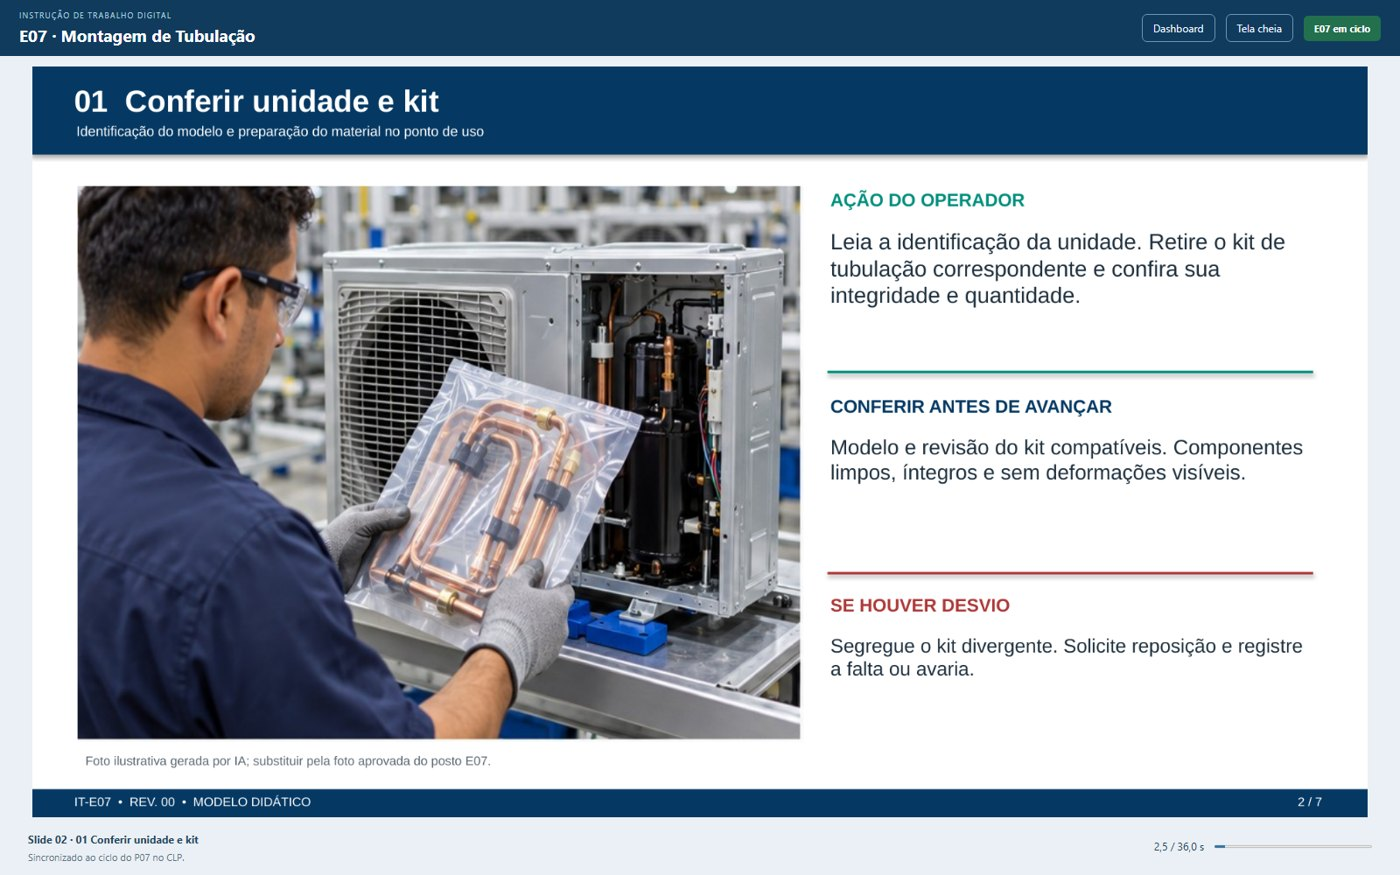
\includegraphics[width=\textwidth]{Imagens/it_running_slide2.jpg}
    \end{minipage}\hfill
    \begin{minipage}{0.49\textwidth}\centering
        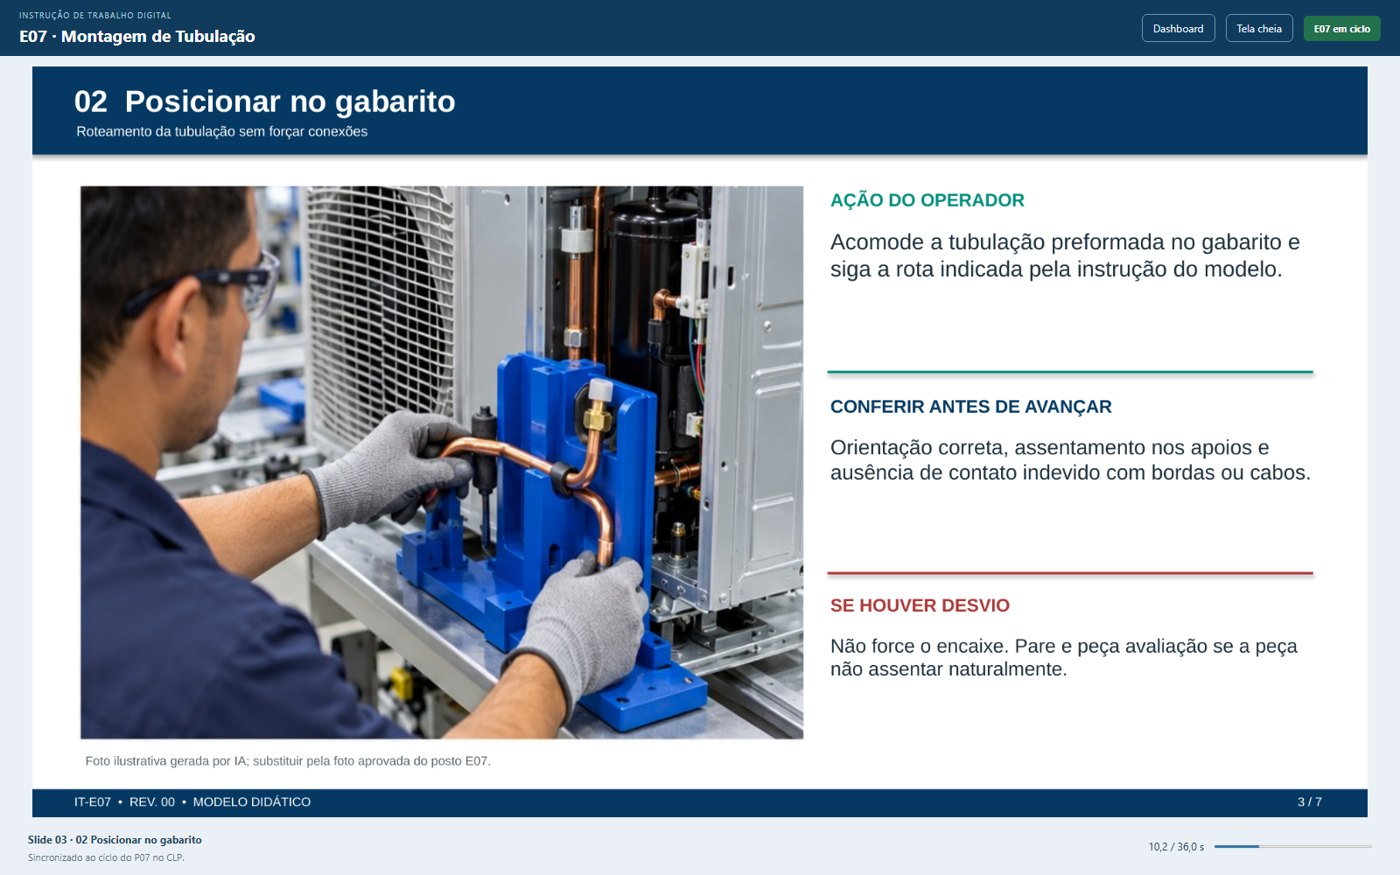
\includegraphics[width=\textwidth]{Imagens/it_running_slide3.jpg}
    \end{minipage}\\[0.2cm]
    \begin{minipage}{0.49\textwidth}\centering
        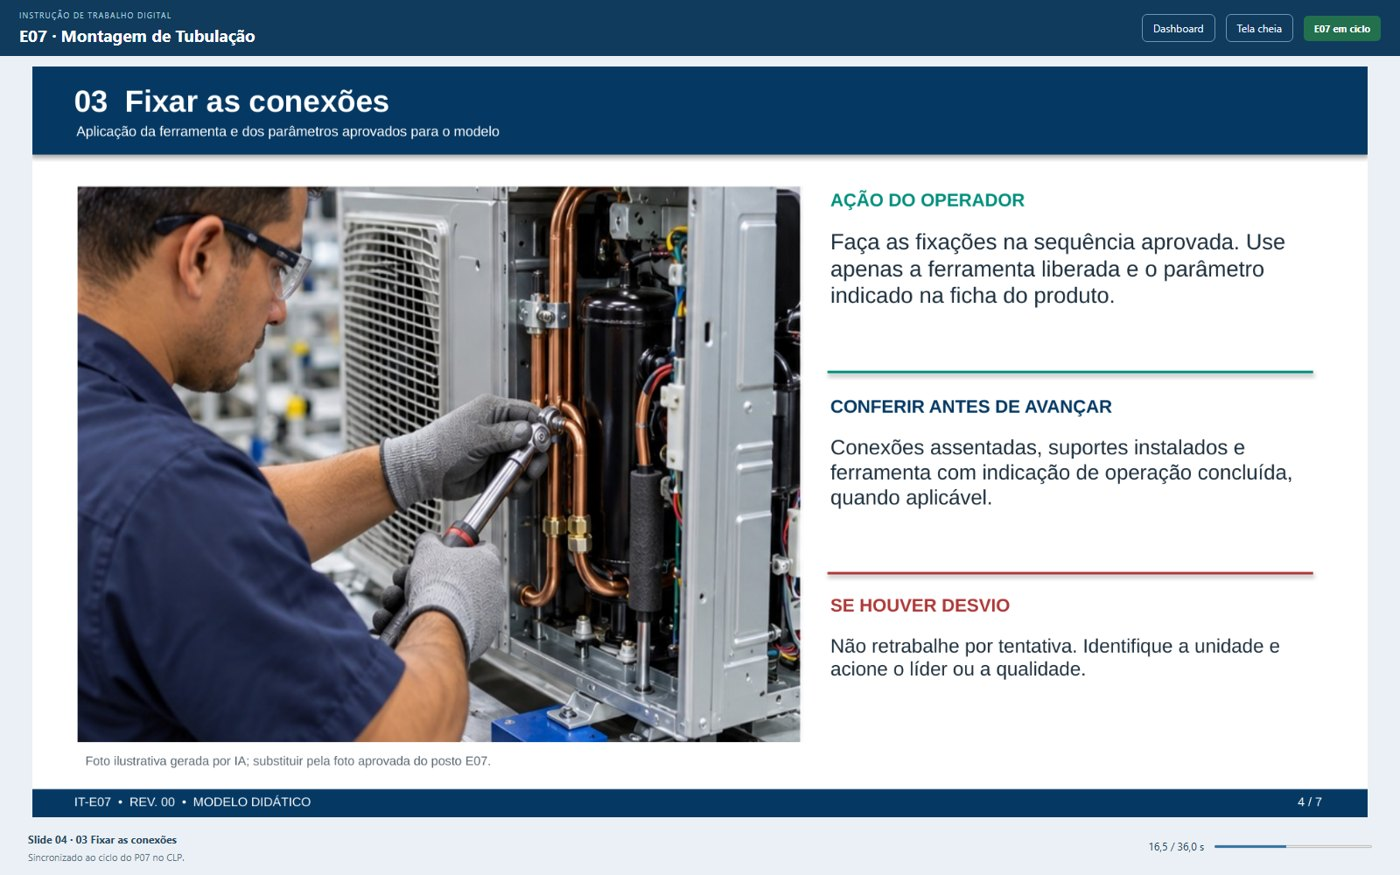
\includegraphics[width=\textwidth]{Imagens/it_running_slide4.jpg}
    \end{minipage}\hfill
    \begin{minipage}{0.49\textwidth}\centering
        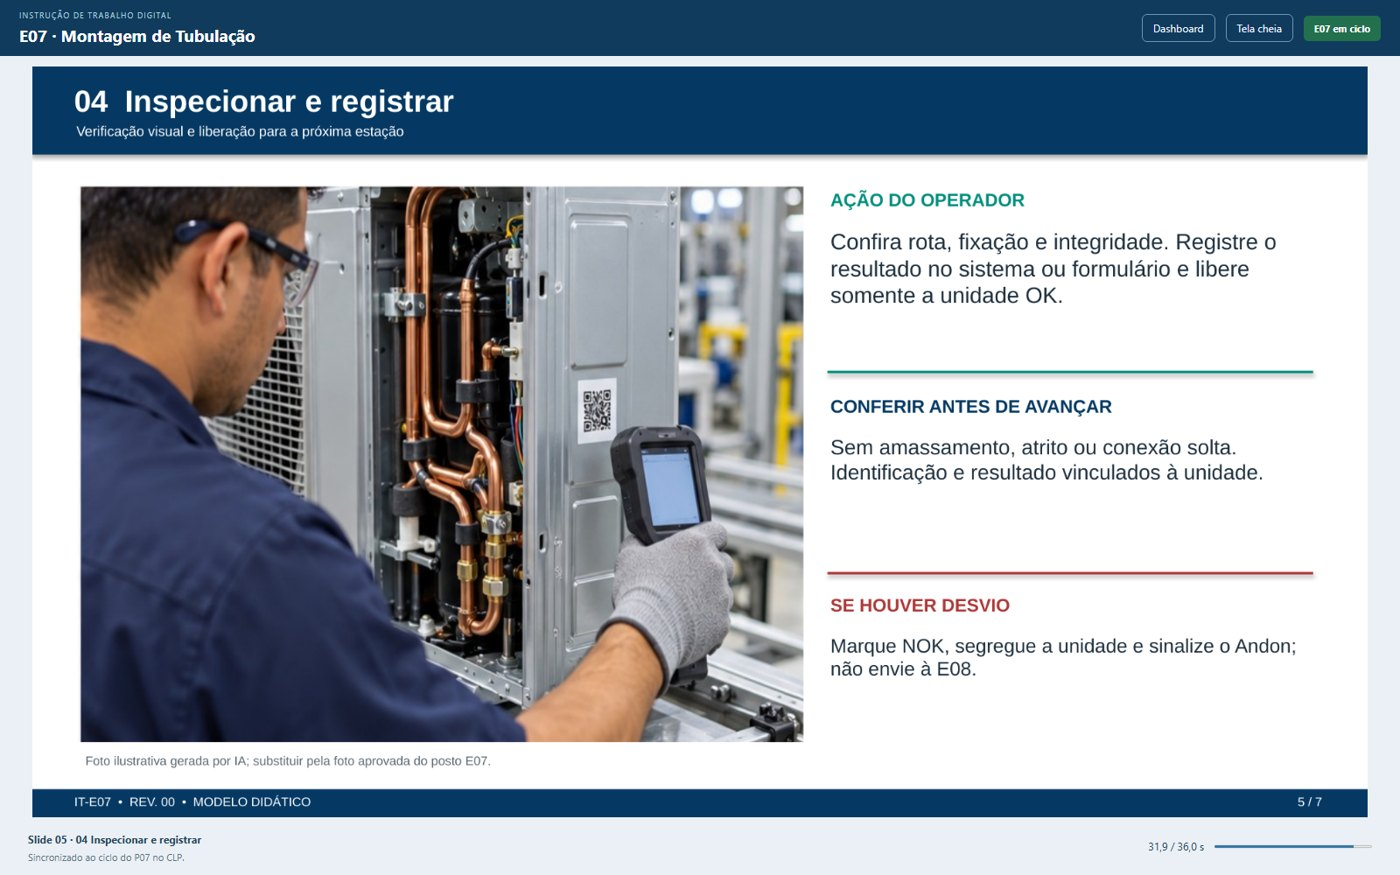
\includegraphics[width=\textwidth]{Imagens/it_running_slide5.jpg}
    \end{minipage}
    \caption{IT Digital durante o ciclo \cod{plc-p07-1}: passos 01 a 04 (slides 2 a 5), com ``E07 em ciclo'' e ``Sincronizado ao ciclo do P07 no CLP''. (arquivos: Imagens/it\_running\_slide2.jpg a it\_running\_slide5.jpg)}
    \label{fig:it1}
\end{figure}

\begin{figure}[H]
    \centering
    \begin{minipage}{0.49\textwidth}\centering
        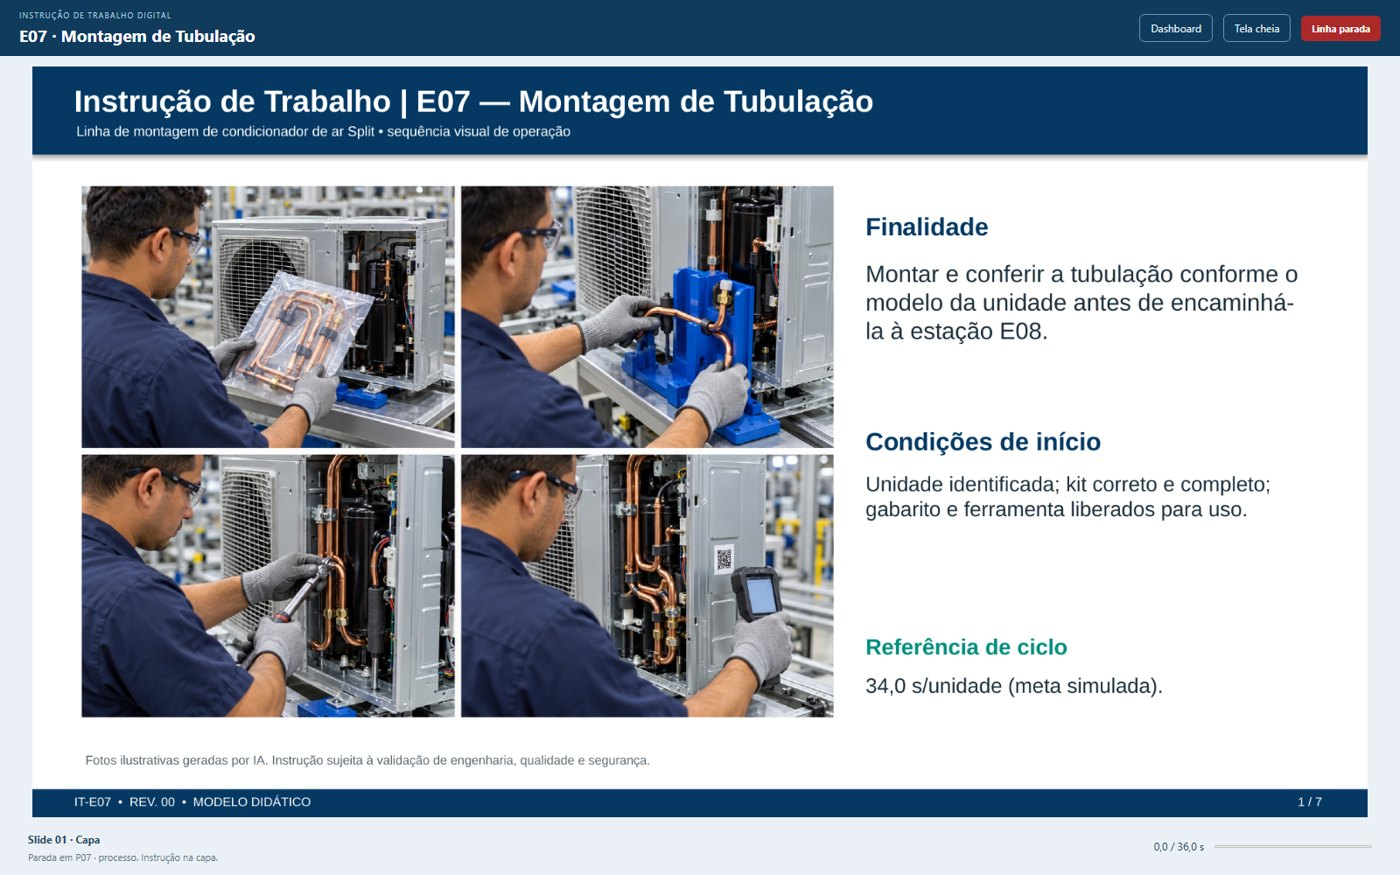
\includegraphics[width=\textwidth]{Imagens/it_paused_slide1.jpg}
    \end{minipage}\hfill
    \begin{minipage}{0.49\textwidth}\centering
        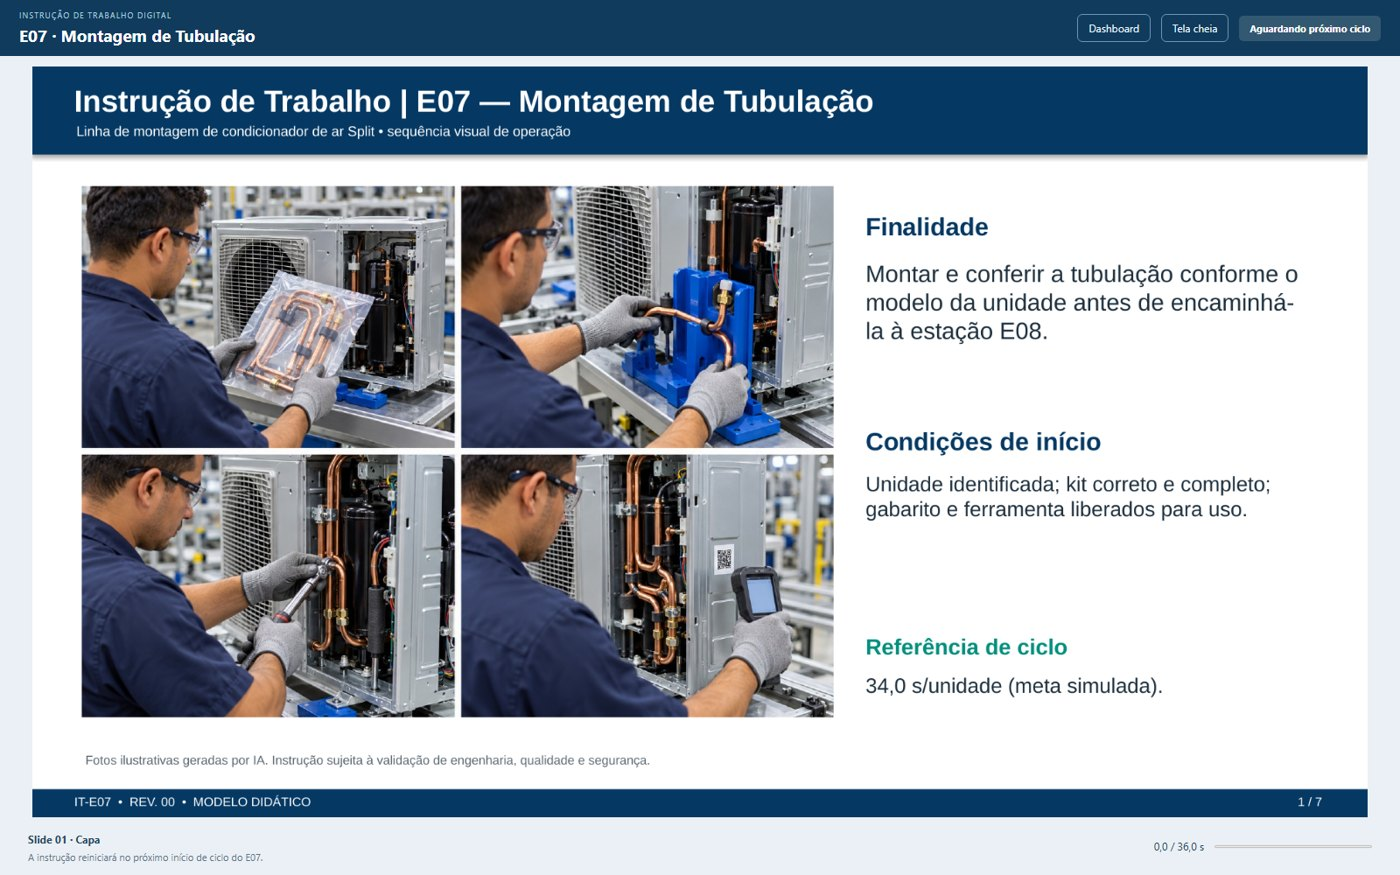
\includegraphics[width=\textwidth]{Imagens/it_interrupted_slide1.jpg}
    \end{minipage}
    \caption{Esquerda: Andon de Processo no P07 - ``Linha parada'', instrução na capa. Direita: após a liberação - ``Aguardando próximo ciclo''. (arquivos: Imagens/it\_paused\_slide1.jpg e it\_interrupted\_slide1.jpg)}
    \label{fig:it2}
\end{figure}

\begin{figure}[H]
    \centering
    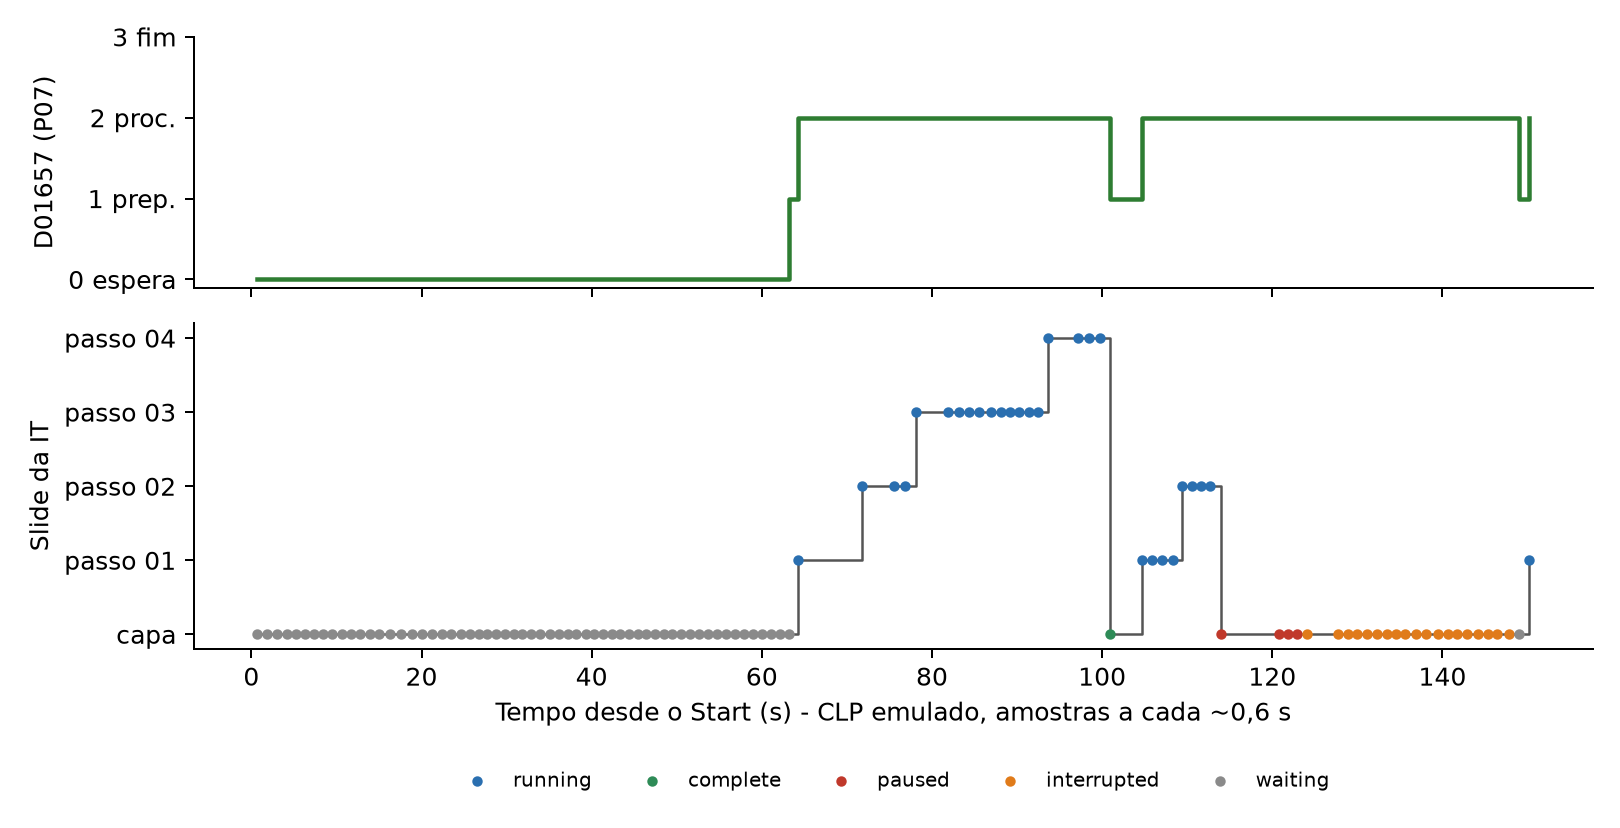
\includegraphics[width=1.00\textwidth]{Imagens/it_sincronizacao_p07.png}
    \caption{Estado do P07 (\cod{D01657}) e slide exibido pela IT Digital ao longo da demonstração. O intervalo mediano entre amostras foi de 1,1 s; o rótulo do eixo traz o valor nominal de 0,6 s. (arquivo: Imagens/it\_sincronizacao\_p07.png)}
    \label{fig:itsync}
\end{figure}

Os quatro testes de \cod{tests/test\_work\_instruction.py} verificam as mesmas regras sem o navegador: a sequência de 36 s, a interrupção por Andon até o próximo início, o descarte de estado inválido e a espera por um ciclo novo após reconexão.

\section{APIs e protocolos (item 2f)}

O sistema expõe quatro interfaces: a API HTTP e os WebSockets do receptor, o espaço de endereços OPC UA do Gateway (e do Desktop), o protocolo binário de Andon sobre TCP e o mapa Modbus do CLP (Tabela \ref{tab:mapa}).

\subsection{API HTTP e WebSocket do receptor}

Implementada em \cod{simulador/web/dashboard.py} (FastAPI). Os corpos são JSON validados por modelos Pydantic com \cod{extra='forbid'}; valores fora do domínio retornam 422. Todas as respostas trazem \cod{Cache-Control: no-store} e \cod{X-Lean-Revision}. Os comandos que acionam o CLP recusam requisições de outra origem (403, proteção contra CSRF a partir de outra página) e aceitam um comando por vez (409); 503 indica Gateway ou banco indisponível e 504, comando sem confirmação do Gateway.

{\footnotesize
\begin{longtable}{|>{\raggedright\arraybackslash}p{1.1cm}|>{\raggedright\arraybackslash}p{4.4cm}|>{\raggedright\arraybackslash}p{6.4cm}|>{\raggedright\arraybackslash}p{2.6cm}|}
\caption{Rotas da API do receptor (porta 8081).}\label{tab:api}\\
\hline
\textbf{Método} & \textbf{Rota} & \textbf{Função} & \textbf{Códigos} \\ \hline
\endfirsthead
\hline
\textbf{Método} & \textbf{Rota} & \textbf{Função} & \textbf{Códigos} \\ \hline
\endhead
GET & \cod{/api/version} & Revisão dos cálculos, recursos e fórmula do desempenho. & 200 \\ \hline
GET & \cod{/api/snapshot} & Estado completo: telemetria OPC UA (12 postos, Andons, Takt, ciclo, estado, contador) e indicadores (\cod{analytics}). & 200 \\ \hline
GET / PUT & \cod{/api/process/production-plan} & Lê ou grava o plano do turno: \cod{production\_target} (inteiro > 0) e \cod{available\_time\_minutes} (> 0). & 200, 422, 503 \\ \hline
GET & \cod{/api/process/cycle-base} & Informa se o controle do CLP está disponível e se a base foi conferida (\cod{BaseCiclosCarregada}). & 200 \\ \hline
POST & \cod{/api/process/cycle-base?filename=} & Recebe a planilha (até 1 MB, \cod{.xlsx}, \cod{.xlsm} ou \cod{.csv}), valida 12 ciclos por posto (0,1 a 6553,5 s) e chama \cod{CarregarBaseCiclos}. & 200, 403, 409, 413, 422, 503, 504 \\ \hline
POST & \cod{/api/process/start} & Chama \cod{IniciarSimulacao}; abre a sessão de medição quando o Ladder confirma. & 200, 403, 409, 503, 504 \\ \hline
POST & \cod{/api/process/clear-base} & Chama \cod{LimparBase} e, confirmado o reset, apaga produção, defeitos e paradas do dia. & 200, 403, 409, 503, 504 \\ \hline
GET / PUT & \cod{/api/process/configuration} & Tempo de ciclo e indicação de protótipo físico dos 12 postos (exatamente 12, valores finitos e positivos). & 200, 422, 503 \\ \hline
POST & \cod{/api/runtime/events} & Eventos do simulador: \cod{andon}, \cod{cycle}, \cod{session\_start}, \cod{production\_plan} e \cod{reset\_day}; idempotente por \cod{event\_id}. & 200, 409, 422, 503 \\ \hline
GET & \cod{/api/instruction/e07} & Estado da IT Digital (slide, status, ciclo, tempo, parada). & 200 \\ \hline
WS & \cod{/ws} & Envia o \cod{/api/snapshot} a cada 1 s. & - \\ \hline
WS & \cod{/ws/instruction/e07} & Envia o estado da IT a cada 100 ms. & - \\ \hline
GET & \cod{/}, \cod{/graficos}, \cod{/instrucao/e07} & Páginas HTML (Dashboard, gráficos por posto e IT Digital). & 200 \\ \hline
\end{longtable}
}

\textbf{Evidência.} A Tabela \ref{tab:apilog} reproduz as chamadas feitas à API real durante a demonstração de 21/11/2026, na ordem em que ocorreram, com as respostas recebidas.

{\footnotesize
\begin{longtable}{|>{\centering\arraybackslash}p{1.2cm}|>{\raggedright\arraybackslash}p{4.6cm}|>{\centering\arraybackslash}p{1.0cm}|>{\raggedright\arraybackslash}p{7.6cm}|}
\caption{Chamadas reais à API (receptor na porta 8091, Gateway real, CLP emulado).}\label{tab:apilog}\\
\hline
\textbf{Hora} & \textbf{Requisição} & \textbf{Código} & \textbf{Resposta (resumo)} \\ \hline
\endfirsthead
\hline
\textbf{Hora} & \textbf{Requisição} & \textbf{Código} & \textbf{Resposta (resumo)} \\ \hline
\endhead
21:14:02 & GET \cod{/api/version} & 200 & \cod{revision: 2026-11-20.01}; recursos \cod{station\_time\_chart}, \cod{reconciled\_downtime}, \cod{digital\_work\_instruction\_e07}. \\ \hline
21:14:03 & PUT \cod{/api/process/production-plan} \{90, 60,0\} & 200 & \cod{\{production\_target: 90, available\_time\_minutes: 60.0\}} \\ \hline
21:14:04 & GET \cod{/api/process/cycle-base} & 200 & \cod{\{available: true, ready: false\}} \\ \hline
21:14:09 & POST \cod{/api/process/cycle-base} (1.223 bytes, \cod{base\_demo.csv}) & 200 & ``Base carregada e conferida no CLP.'' - 288 palavras gravadas e relidas em 12 blocos ($\approx$5,3 s). \\ \hline
21:14:09 & GET \cod{/api/process/cycle-base} & 200 & \cod{\{available: true, ready: true\}} \\ \hline
21:14:10 & POST \cod{/api/process/start} com \cod{Origin: http://evil.example} & \textbf{403} & ``Abra a dashboard para executar este comando do CLP.'' - recusado, nenhum pulso enviado. \\ \hline
21:14:13 & POST \cod{/api/process/start} & 200 & \cod{\{result: 0, confirmed: true\}} ``Início confirmado pelo CLP.'' ($\approx$3,0 s: pulso de 2 s em \cod{P10002} e confirmação pelo estado 2). \\ \hline
21:18:20 & GET \cod{/api/instruction/e07} & 200 & \cod{source: plc, slide: 4, status: running, cycle\_id: plc-p07-4, elapsed\_seconds: 28.59} \\ \hline
21:18:20 & POST \cod{/api/runtime/events} com \cod{station: 13} & \textbf{422} & ``Input should be less than or equal to 12'' - evento inválido rejeitado pela validação. \\ \hline
21:18:23 & POST \cod{/api/process/clear-base} & 200 & ``Base do dia limpa. Aguardando o próximo Start confirmado.'' ($\approx$2,7 s). \\ \hline
21:18:27 & GET \cod{/api/snapshot} & 200 & \cod{connected: true, plc\_production\_count: 0} (contador zerado pelo reset). \\ \hline
\end{longtable}
}

\subsection{OPC UA}

O Gateway (e o Desktop, no modo simulado) publica o endpoint \cod{opc.tcp://<gateway>:4840/mock-linha/}, namespace \cod{urn:mock-linha:telemetria:v1}, com uma única política: \cod{Basic256Sha256} em modo \cod{SignAndEncrypt}. Não há endpoint \cod{None} nem modo somente assinado. O servidor só aceita clientes cujo certificado esteja na pasta de confiança, dentro da validade, com \cod{ExtendedKeyUsage = clientAuth} e com \cod{ApplicationUri} igual ao da sessão; o cliente do receptor, por sua vez, fixa o certificado esperado do servidor. As variáveis são somente leitura para os clientes (Tabela \ref{tab:opcua}).

{\footnotesize
\begin{longtable}{|>{\raggedright\arraybackslash}p{5.4cm}|>{\raggedright\arraybackslash}p{2.6cm}|>{\raggedright\arraybackslash}p{6.6cm}|}
\caption{Espaço de endereços OPC UA (NodeIds do tipo \textit{string}).}\label{tab:opcua}\\
\hline
\textbf{NodeId} & \textbf{Tipo} & \textbf{Origem / efeito} \\ \hline
\endfirsthead
\hline
\textbf{NodeId} & \textbf{Tipo} & \textbf{Origem / efeito} \\ \hline
\endhead
\cod{Pnn/Andon/Qualidade}, \cod{.../Equipamento}, \cod{.../Processo}, \cod{.../Material} (nn = 01..12) & Boolean (48) & Bits de \cod{D109}-\cod{D111}. \\ \hline
\cod{Pnn/TaktTime}, \cod{Pnn/UltimoCiclo} & Double (24) & UInt32 de \cod{D113}-\cod{D160} convertidos para segundos. \\ \hline
\cod{Linha/StatusProcesso} & vetor de 12 Int32 & \cod{D1651}-\cod{D1662}; -1 antes da primeira leitura válida. \\ \hline
\cod{Linha/TotalProduzido} & Int32 & \cod{D16052}; -1 antes da primeira leitura válida. \\ \hline
\cod{Linha/CarregarBaseCiclos(144 tempos)} & método & Grava e confere \cod{D17001}-\cod{D17288}. \\ \hline
\cod{Linha/BaseCiclosCarregada()} & método & Retorna se os 12 blocos foram conferidos. \\ \hline
\cod{Linha/IniciarSimulacao()} & método & Pulso de 2 s em \cod{P10002}; retorna o instante da confirmação. \\ \hline
\cod{Linha/LimparBase()} & método & Pulso de 2 s em \cod{P10003}; confere \cod{D16052 = 0}. \\ \hline
\cod{Linha/DefinirVelocidadeMotor(UInt16 0..100)} & método & Escreve \cod{D1200}. \\ \hline
\cod{Linha/DefinirParada(Boolean)} & método & Altera somente o bit 0 de \cod{D1201} (leitura-modificação-escrita). \\ \hline
\end{longtable}
}

Os métodos entram na fila do \cod{plc\_poller} e são executados na mesma \textit{thread} da porta serial; o cliente só recebe sucesso depois da confirmação da escrita Modbus. \textbf{Evidência:} nas duas execuções da demonstração o cliente do receptor conectou-se ao Gateway real (``Cliente OPC UA: conectado''; no Gateway, ``OPC UA: active and secure'') e os métodos \cod{CarregarBaseCiclos}, \cod{BaseCiclosCarregada}, \cod{IniciarSimulacao} e \cod{LimparBase} foram chamados com sucesso pela API (Tabela \ref{tab:apilog}). Os testes \cod{test\_secure\_server\_exposes\_and\_updates\_the\_same\_72\_nodes}, \cod{test\_wrong\_server\_certificate\_is\_rejected}, \cod{test\_unknown\_client\_certificate\_is\_rejected} e \cod{test\_expired\_client\_certificate\_is\_rejected} comprovam a publicação dos nós e a recusa de certificados desconhecidos, vencidos ou de servidor incorreto.

\subsection{Protocolo binário de Andon (TCP)}

Cada evento tem exatamente 16 bytes, com inteiros de 16 bits em \textit{big-endian} e data e hora em BCD (Tabela \ref{tab:decode}): tipo (\cod{00 01} do CLP ou do Desktop; \cod{00 02} para eventos do simulador via API), posto (1 a 12), mês, ano, hora, dia, segundo, minuto, século e dia da semana (0 = domingo), botão (1 Qualidade, 2 Equipamento, 3 Processo, 4 Material) e estado (1 ligado, 2 desligado). O receptor lê os 16 bytes, grava a recepção no SQLite e só então responde com o ACK de 22 bytes ASCII - vinte caracteres \cod{0} seguidos de \cod{15}, sem quebra de linha. Formato inválido, posto ou botão desconhecido e falha de banco fecham a conexão sem ACK, e o remetente tenta de novo. O pedido de hora é \cod{00 01} seguido de 14 bytes zero e a resposta, oito bytes BCD.

A política do receptor para casos excepcionais (\cod{test\_reference\_receiver\_exception\_policy}) é: ON com ocorrência já aberta $\rightarrow$ \cod{ON\_REPETIDO}; OFF sem ocorrência aberta $\rightarrow$ \cod{OFF\_SEM\_ABERTURA}; evento anterior ao último da mesma chave posto/botão $\rightarrow$ \cod{ATRASADO}. Todos recebem ACK. Um reenvio idêntico (mesmos 16 bytes, por exemplo após a perda do ACK) é reconhecido pela tabela \cod{processed\_event} e recebe novo ACK sem ser aplicado outra vez (\cod{test\_exact\_retransmission\_is\_acked\_without\_reapplying\_event}).

\textbf{Limite conhecido.} O pacote não tem identificador de evento. Dois eventos legítimos idênticos no mesmo segundo produziriam os mesmos 16 bytes; por isso o sistema garante fila durável e entrega com nova tentativa, mas não processamento exatamente uma vez. Para essa garantia, o protocolo precisaria incluir um identificador.

\section{Verificação e testes automatizados}

Os testes foram executados em 21/11/2026 com \cod{pytest 8.3.5} no ambiente descrito na seção \ref{sec:materiais}, a partir das pastas \cod{simulador/} e \cod{hardware/} (\cod{..\textbackslash venv\textbackslash Scripts\textbackslash python.exe -m pytest -v}). Nenhum teste exige hardware: o Modbus, o TCP, o SNTP e o OPC UA são exercitados com simuladores locais e servidores reais em portas efêmeras.

\begin{itemize}
    \item \textbf{Simulador:} 98 testes, 98 aprovados, 0 falhas, em 28,2 s.
    \item \textbf{Gateway:} 66 testes, 64 aprovados, 0 falhas e 2 pulados, em 8,5 s. Os dois testes pulados (\cod{test\_gpio\_driver\_starts\_disabled\_and\_releases\_pins} e \cod{test\_gpio\_cleanup\_continues\_after\_one\_device\_close\_fails}) dependem da biblioteca \cod{gpiozero}, instalada somente na Raspberry Pi (\cod{sys\_platform == 'linux'}).
\end{itemize}

{\footnotesize
\begin{longtable}{|>{\raggedright\arraybackslash}p{2.0cm}|>{\raggedright\arraybackslash}p{4.2cm}|>{\centering\arraybackslash}p{1.6cm}|>{\raggedright\arraybackslash}p{6.8cm}|}
\caption{Testes automatizados por arquivo (resultado de \cod{--junitxml}).}\label{tab:testes}\\
\hline
\textbf{Projeto} & \textbf{Arquivo} & \textbf{Aprovados} & \textbf{O que verifica} \\ \hline
\endfirsthead
\hline
\textbf{Projeto} & \textbf{Arquivo} & \textbf{Aprovados} & \textbf{O que verifica} \\ \hline
\endhead
Simulador & \cod{test\_analytics.py} & 6 & Contador absoluto do CLP, união de paradas sobrepostas, ocorrência aberta e estabilidade por categoria. \\ \hline
Simulador & \cod{test\_base\_import.py} & 4 & Planilha em pares de linhas e de colunas, primeira aba do .xlsx e par incompleto. \\ \hline
Simulador & \cod{test\_bcd.py} & 11 & Ida e volta BCD de 0 a 99 e rejeição de valores e nibbles inválidos. \\ \hline
Simulador & \cod{test\_certificates.py} & 1 & Certificado de cliente vencido é recusado. \\ \hline
Simulador & \cod{test\_database.py} & 4 & Clique atômico com fila, reinício com fila pendente, rollback e categorias simultâneas. \\ \hline
Simulador & \cod{test\_example\_bases.py} & 1 & Geração e importação das planilhas de exemplo. \\ \hline
Simulador & \cod{test\_opcua\_controls.py} & 2 & Métodos de motor e parada com tipos explícitos e validação. \\ \hline
Simulador & \cod{test\_opcua\_integration.py} & 4 & 72 nós somente leitura, certificado de servidor errado, cliente desconhecido e assinatura pela Dashboard. \\ \hline
Simulador & \cod{test\_process\_configuration.py} & 41 & Importação e Start pelo Gateway, persistência, plano do turno, reset e 30 casos de valores inválidos. \\ \hline
Simulador & \cod{test\_reference\_receiver.py} & 5 & Política de exceções, COMMIT antes do ACK, reenvio idêntico e formatos 00 01/00 02. \\ \hline
Simulador & \cod{test\_tcp\_codec.py} & 5 & Exemplos ON/OFF documentados, posto 12 como 00 0C, dia da semana e pedido de hora. \\ \hline
Simulador & \cod{test\_tcp\_sender.py} & 1 & Reenvio do primeiro evento preservando a ordem FIFO. \\ \hline
Simulador & \cod{test\_telemetry.py} & 3 & Telemetria alterada somente pelo OPC UA e ordem dos 12 estados. \\ \hline
Simulador & \cod{test\_ui.py} & 4 & Janela com 12 postos, edição de métricas, importação com intervalo de 1 s. \\ \hline
Simulador & \cod{test\_web\_dashboard.py} & 2 & Página, API e WebSocket; página de gráficos e arquivos da E07. \\ \hline
Simulador & \cod{test\_work\_instruction.py} & 4 & Sequência de 36 s, interrupção por Andon, estado inválido e reconexão. \\ \hline
Gateway & \cod{test\_application.py} & 1 & Partida e parada do serviço sem hardware. \\ \hline
Gateway & \cod{test\_config.py} & 1 & Configuração de exemplo segura (Modbus desabilitado) e portável. \\ \hline
Gateway & \cod{test\_modbus\_transport.py} & 16 & Endereços, FC03/04/05/06/16, base de ciclos, relógio, ACK, D1200 e bit 0 de D1201. \\ \hline
Gateway & \cod{test\_motor\_output.py} & 10 (+2 pulados) & Rampas, interrupção por novo comando ou falha, desligamento e validação de velocidade. \\ \hline
Gateway & \cod{test\_ntp\_client.py} & 5 & Decodificação SNTP, rejeição de resposta não sincronizada, nova tentativa e hora do sistema uma única vez. \\ \hline
Gateway & \cod{test\_opcua\_integration.py} & 1 & Servidor seguro com os mesmos 72 nós atualizados. \\ \hline
Gateway & \cod{test\_persistence.py} & 3 & Captura durável, deduplicação do pacote, colisão de CRC32 e evento pendente após reinício. \\ \hline
Gateway & \cod{test\_plc\_clock.py} & 2 & Palavras BCD de DATEWR e segunda-feira = 1. \\ \hline
Gateway & \cod{test\_plc\_poller.py} & 15 & COMMIT antes de P10000, ACK repetido sem perda, Start, reset e serialização de comandos. \\ \hline
Gateway & \cod{test\_protocol.py} & 2 & Pacote de 16 bytes e identificador com CRC32. \\ \hline
Gateway & \cod{test\_register\_map.py} & 5 & Nibbles de Andon, UInt32 até o P12, ordem de palavras e D112. \\ \hline
Gateway & \cod{test\_tcp\_sender.py} & 3 & Pacote exato com ACK fragmentado, ACK inválido e FIFO persistente. \\ \hline
\end{longtable}
}

Os testes complementam as execuções descritas nas seções anteriores: os comportamentos que dependem de falhas difíceis de provocar no hardware - colisão de CRC32, queda da conexão entre o COMMIT e o ACK, certificado vencido, ACK TCP fragmentado, falha do banco no meio de um clique - são verificados aqui de forma determinística.

\newpage

\section{Conclusões}

\begin{itemize}
    \item Para o Cenário 25, linha de montagem de ar-condicionado com 12 postos, o sistema desenvolvido pela Equipe 4 integra o CLP LS XGK, a Raspberry Pi e a supervisão no Windows por protocolos padronizados (Modbus RTU, OPC UA com \cod{Basic256Sha256}/\cod{SignAndEncrypt}, SNTP) e por um protocolo binário de Andon de 16 bytes com ACK. O Desktop fala os mesmos protocolos do Gateway, de modo que o receptor e a Dashboard funcionam sem alteração de código com a linha real ou com o simulador. No simulador, porém, não há os nós e métodos \cod{Linha/*}: o estado dos postos, o contador de produção, a IT Digital sincronizada e os comandos de base, Start e reset exigem o Gateway.
    \item Na execução com o CLP real, os 18 eventos de Andon foram capturados, confirmados ao CLP em 13,4 a 17,3 ms e entregues ao receptor em 23,4 a 39,9 ms, sem nova tentativa. Durante uma perda de comunicação de 1 h 38 min, quatro eventos ficaram retidos na FIFO do CLP e foram entregues em ordem na reconexão: a combinação ``fila no Ladder + COMMIT antes do \cod{P10000} + fila SQLite no Gateway + ACK TCP após persistência'' não perdeu nem duplicou eventos.
    \item O Gateway mostrou-se resiliente: manteve OPC UA e TCP ativos sem o CLP, tentou reabrir a porta a cada 2 s (4.444 tentativas registradas), sincronizou o relógio do CLP logo após a reconexão e encerrou de forma ordenada.
    \item A Dashboard calcula Disponibilidade, Desempenho, Qualidade e OEE a partir dos estados e do contador do CLP; a conferência manual da Figura \ref{fig:dash3} reproduz os valores exibidos (84,1 \%, 40,0 \%, 66,7 \% e 22,4 \%). Os estados dos 12 postos tornam visíveis o fluxo de peças e o gargalo (P07), objetivo central do acompanhamento \textit{Lean}.
    \item A IT Digital E07 acompanhou o ciclo do P07 no CLP emulado com trocas de slide até 0,9 s após o limite teórico e respeitou as regras de parada por Andon e de espera pelo próximo ciclo.
    \item A API rejeitou comandos de outra origem (403) e dados fora do domínio (422), e os comandos de base, Start e reset só foram confirmados após a verificação no CLP. As 162 verificações automatizadas aprovadas (98 do Simulador e 64 do Gateway) cobrem os casos de falha difíceis de reproduzir no hardware.
    \item Limitações: as capturas de tela e as medições da Dashboard e da IT Digital foram obtidas com o Gateway real e um CLP emulado, que simplifica o Ladder; as redes completas dos postos 03 a 06 e 12 não constam nas capturas do XG5000; e o protocolo de Andon não tem identificador de evento, o que impede garantir processamento exatamente uma vez. O gêmeo digital e a conexão entre gêmeos (T2T) não foram implementados, e o log e os bancos originais da execução real não acompanham a entrega, que inclui apenas o extrato dos 18 eventos. A amostra de ciclos físicos da E07 ainda não foi coletada, portanto não há comparação estatística entre os ciclos reais e os simulados, e a IT Digital, de 36 s, excede a meta de 34 s da E07 e o Takt de 34,6 s do cenário. Recomenda-se repetir as capturas com a linha física completa, coletar ao menos 30 ciclos físicos, compatibilizar a duração da IT e incluir um identificador no protocolo antes de uma homologação.
\end{itemize}

\section{Referências}

\begin{itemize}
    \item LS ELECTRIC. \textit{XGK/XGB Instructions and Programming - User's Manual}. Instruções \cod{DATERD}, \cod{DATEWR}, \cod{FIWR}, \cod{FIFRDP} e \cod{FMOV}.
    \item LS ELECTRIC. \textit{XG5000 - Programming Software}, versão 4.74.
    \item MODBUS ORGANIZATION. \textit{MODBUS Application Protocol Specification V1.1b3}, 2012; \textit{MODBUS over Serial Line Specification and Implementation Guide V1.02}, 2006.
    \item OPC FOUNDATION. \textit{OPC Unified Architecture Specification}, IEC 62541. Parte 2 (Security Model) e Parte 4 (Services).
    \item MILLS, D. et al. \textit{Network Time Protocol Version 4: Protocol and Algorithms Specification}. RFC 5905, IETF, 2010.
    \item NAKAJIMA, S. \textit{Introduction to TPM: Total Productive Maintenance}. Cambridge: Productivity Press, 1988 (definição do OEE).
    \item ROTHER, M.; SHOOK, J. \textit{Learning to See: Value Stream Mapping to Add Value and Eliminate Muda}. Lean Enterprise Institute, 1999.
    \item TEXAS INSTRUMENTS. \textit{DRV8825 Stepper Motor Controller IC - Datasheet}, SLVSA73F.
    \item Bibliotecas: asyncua 1.1.5, pymodbus 3.11.3, FastAPI 0.115.11, PyQt6 6.8.1, cryptography 44.0.2, gpiozero 2.0.1, pigpio 1.78.
    \item Código-fonte do projeto: \cod{hardware/}, \cod{simulador/} e documentação em \cod{docs/} (\cod{ARQUITETURA\_COMUNICACAO\_LINHA.md}, \cod{DOCUMENTACAO\_CLP\_LS\_XGK.md}, \cod{FLUXOGRAMA\_MAQUINA\_ESTADOS\_CLP.md}).
\end{itemize}
\newpage

\section*{Anexo - Tabelas e figuras complementares}
\addcontentsline{toc}{section}{Anexo - Tabelas e figuras complementares}
\setcounter{table}{0}\renewcommand{\thetable}{A\arabic{table}}
\setcounter{figure}{0}\renewcommand{\thefigure}{A\arabic{figure}}

{\footnotesize
\begin{longtable}{|>{\centering\arraybackslash}p{0.5cm}|>{\centering\arraybackslash}p{2.2cm}|>{\centering\arraybackslash}p{0.8cm}|>{\raggedright\arraybackslash}p{1.8cm}|>{\centering\arraybackslash}p{0.8cm}|>{\raggedright\arraybackslash}p{4.6cm}|>{\centering\arraybackslash}p{1.3cm}|>{\centering\arraybackslash}p{1.3cm}|}
\caption{Os 18 eventos de Andon capturados no CLP real pelo Gateway \cod{LINHA\_A} (\cod{hardware/data/gateway.db}, 27/09/2026). ``ACK CLP'' e ``ACK TCP'': milissegundos desde a gravação no SQLite.}\\
\hline
\textbf{Id} & \textbf{Ocorrência (CLP)} & \textbf{Posto} & \textbf{Botão} & \textbf{Estado} & \textbf{Pacote (hex)} & \textbf{ACK CLP} & \textbf{ACK TCP} \\ \hline
\endfirsthead
\hline
\textbf{Id} & \textbf{Ocorrência (CLP)} & \textbf{Posto} & \textbf{Botão} & \textbf{Estado} & \textbf{Pacote (hex)} & \textbf{ACK CLP} & \textbf{ACK TCP} \\ \hline
\endhead
1 & 2026-09-27 16:59:03 & P05 & Processo & ON & \cod{00 01 00 05 09 26 16 27 03 59 20 00 00 03 00 01} & 15,3 & 36,7 \\ \hline
2 & 2026-09-27 17:01:41 & P05 & Processo & OFF & \cod{00 01 00 05 09 26 17 27 41 01 20 00 00 03 00 02} & 15,2 & 39,3 \\ \hline
3 & 2026-09-27 17:01:51 & P05 & Material & ON & \cod{00 01 00 05 09 26 17 27 51 01 20 00 00 04 00 01} & 15,6 & 33,2 \\ \hline
4 & 2026-09-27 17:02:01 & P05 & Material & OFF & \cod{00 01 00 05 09 26 17 27 01 02 20 00 00 04 00 02} & 15,8 & 25,8 \\ \hline
5 & 2026-09-27 17:04:42 & P05 & Processo & ON & \cod{00 01 00 05 09 26 17 27 42 04 20 00 00 03 00 01} & 15,6 & 33,6 \\ \hline
6 & 2026-09-27 17:04:59 & P05 & Processo & OFF & \cod{00 01 00 05 09 26 17 27 59 04 20 00 00 03 00 02} & 17,3 & 28,9 \\ \hline
7 & 2026-09-27 17:05:07 & P05 & Equipamento & ON & \cod{00 01 00 05 09 26 17 27 07 05 20 00 00 02 00 01} & 16,7 & 35,3 \\ \hline
8 & 2026-09-27 17:05:22 & P05 & Equipamento & OFF & \cod{00 01 00 05 09 26 17 27 22 05 20 00 00 02 00 02} & 16,0 & 37,0 \\ \hline
9 & 2026-09-27 17:09:25 & P05 & Equipamento & ON & \cod{00 01 00 05 09 26 17 27 25 09 20 00 00 02 00 01} & 16,4 & 36,2 \\ \hline
10 & 2026-09-27 17:09:37 & P05 & Equipamento & OFF & \cod{00 01 00 05 09 26 17 27 37 09 20 00 00 02 00 02} & 17,0 & 36,6 \\ \hline
11 & 2026-09-27 17:09:47 & P05 & Processo & ON & \cod{00 01 00 05 09 26 17 27 47 09 20 00 00 03 00 01} & 16,3 & 35,8 \\ \hline
12 & 2026-09-27 17:09:53 & P05 & Processo & OFF & \cod{00 01 00 05 09 26 17 27 53 09 20 00 00 03 00 02} & 15,7 & 23,7 \\ \hline
13 & 2026-09-27 22:19:09 & P05 & Qualidade & ON & \cod{00 01 00 05 09 26 22 27 09 19 20 00 00 01 00 01} & 13,4 & 23,4 \\ \hline
14 & 2026-09-27 22:19:42 & P05 & Qualidade & OFF & \cod{00 01 00 05 09 26 22 27 42 19 20 00 00 01 00 02} & 14,9 & 24,1 \\ \hline
15 & 2026-09-27 22:19:54 & P05 & Equipamento & ON & \cod{00 01 00 05 09 26 22 27 54 19 20 00 00 02 00 01} & 16,0 & 25,5 \\ \hline
16 & 2026-09-27 22:19:56 & P05 & Equipamento & OFF & \cod{00 01 00 05 09 26 22 27 56 19 20 00 00 02 00 02} & 15,3 & 24,3 \\ \hline
17 & 2026-09-27 22:26:37 & P05 & Qualidade & ON & \cod{00 01 00 05 09 26 22 27 37 26 20 00 00 01 00 01} & 16,2 & 34,2 \\ \hline
18 & 2026-09-27 22:26:44 & P05 & Qualidade & OFF & \cod{00 01 00 05 09 26 22 27 44 26 20 00 00 01 00 02} & 16,3 & 39,9 \\ \hline
\end{longtable}
}

\noindent As figuras a seguir completam as capturas do projeto \cod{LAB\_NEW\_UPDATED} no XG5000 apresentadas na seção 3.

\begin{figure}[H]
    \centering
    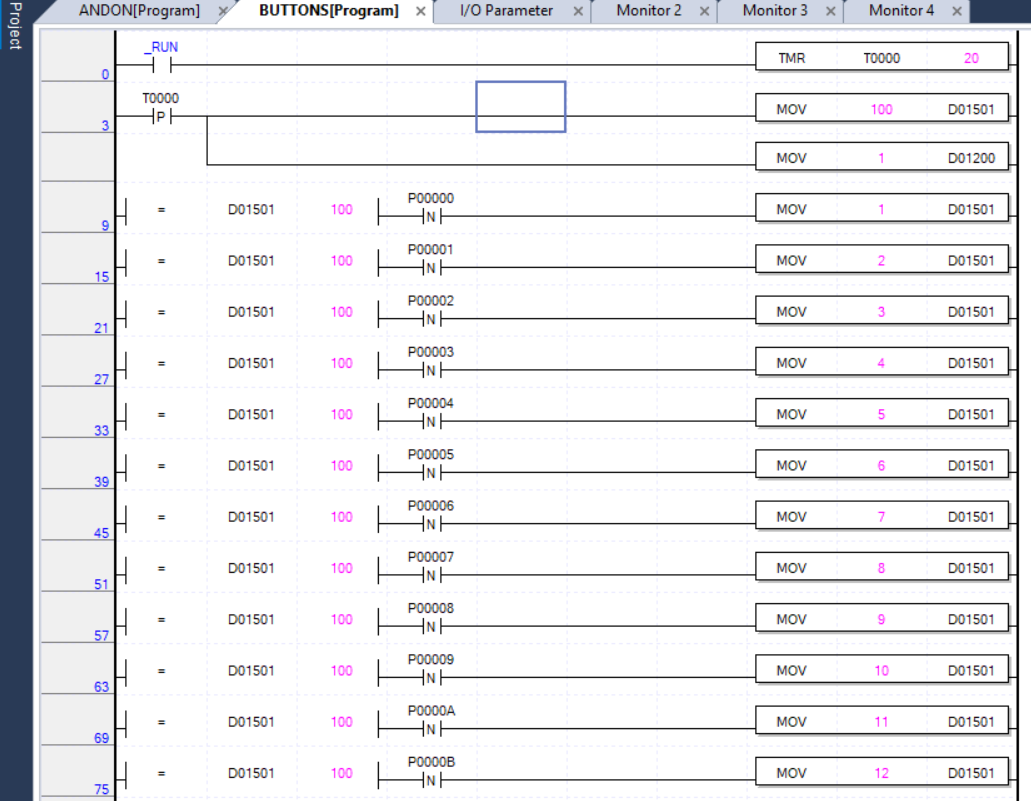
\includegraphics[width=0.72\textwidth]{Imagens/clp_04_buttons_inicializacao.png}
    \caption{BUTTONS: inicialização de \cod{D01501} em 100 e bordas de descida que selecionam os estados 1 a 12. (arquivo: Imagens/clp\_04\_buttons\_inicializacao.png)}
\end{figure}

\begin{figure}[H]
    \centering
    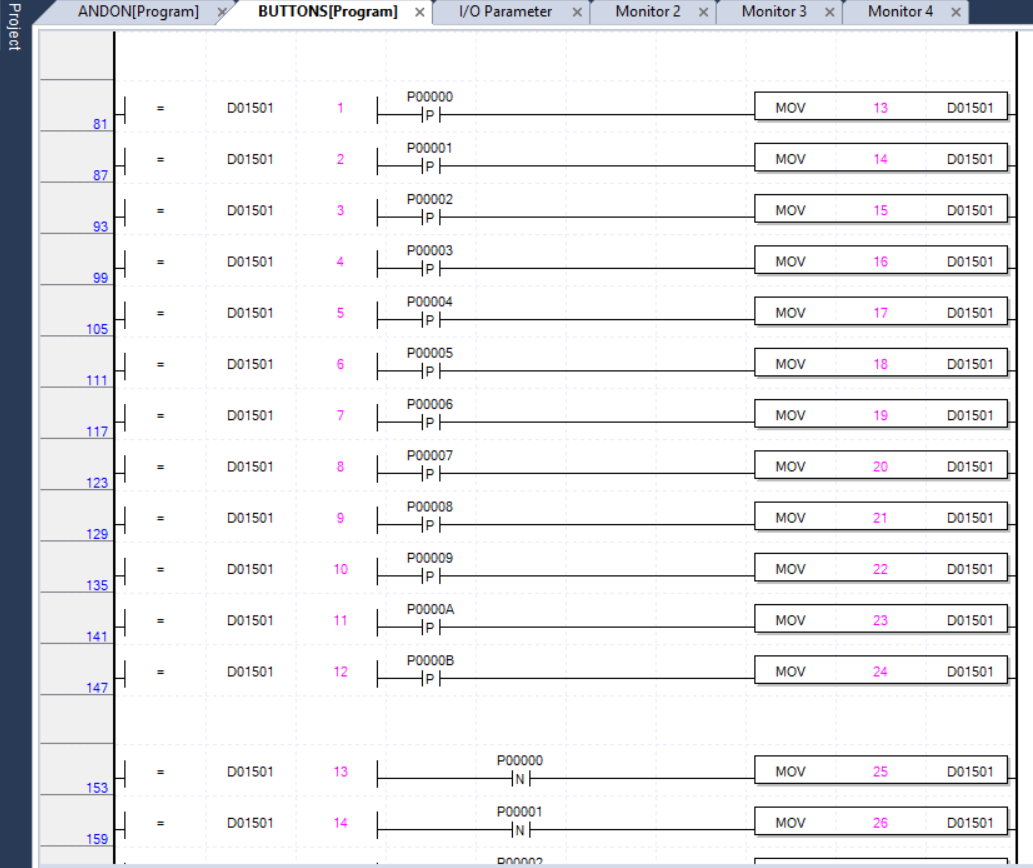
\includegraphics[width=0.72\textwidth]{Imagens/clp_05_buttons_borda_subida.png}
    \caption{BUTTONS: bordas de subida levam \cod{D01501} de 1-12 para 13-24. (arquivo: Imagens/clp\_05\_buttons\_borda\_subida.png)}
\end{figure}

\begin{figure}[H]
    \centering
    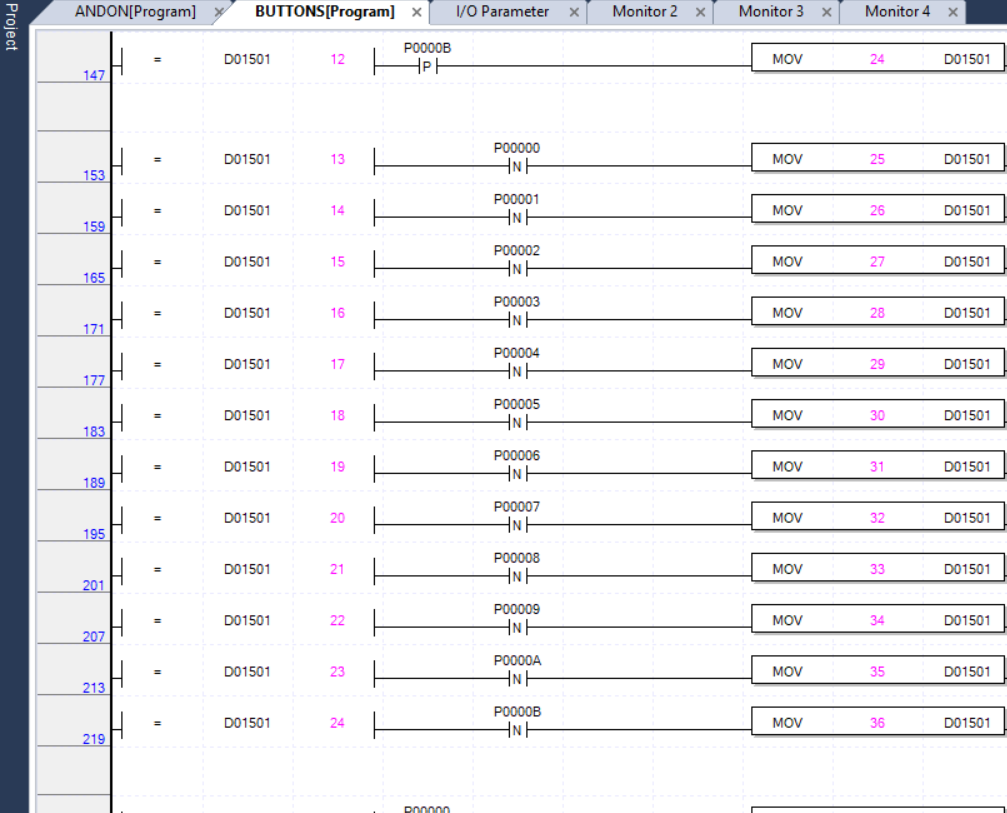
\includegraphics[width=0.72\textwidth]{Imagens/clp_06_buttons_borda_descida.png}
    \caption{BUTTONS: bordas de descida seguintes levam \cod{D01501} de 13-24 para 25-36. (arquivo: Imagens/clp\_06\_buttons\_borda\_descida.png)}
\end{figure}

\begin{figure}[H]
    \centering
    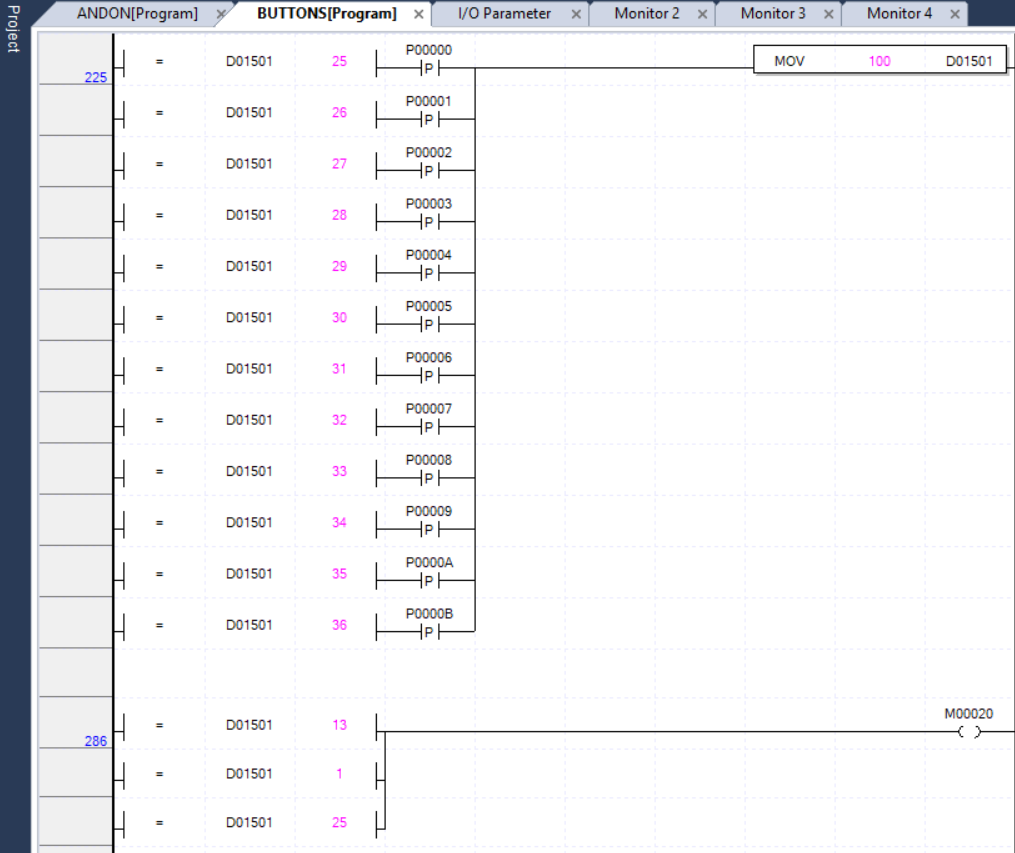
\includegraphics[width=0.72\textwidth]{Imagens/clp_07_buttons_retorno.png}
    \caption{BUTTONS: nos estados 25-36, a subida da entrada devolve \cod{D01501} a 100. (arquivo: Imagens/clp\_07\_buttons\_retorno.png)}
\end{figure}

\begin{figure}[H]
    \centering
    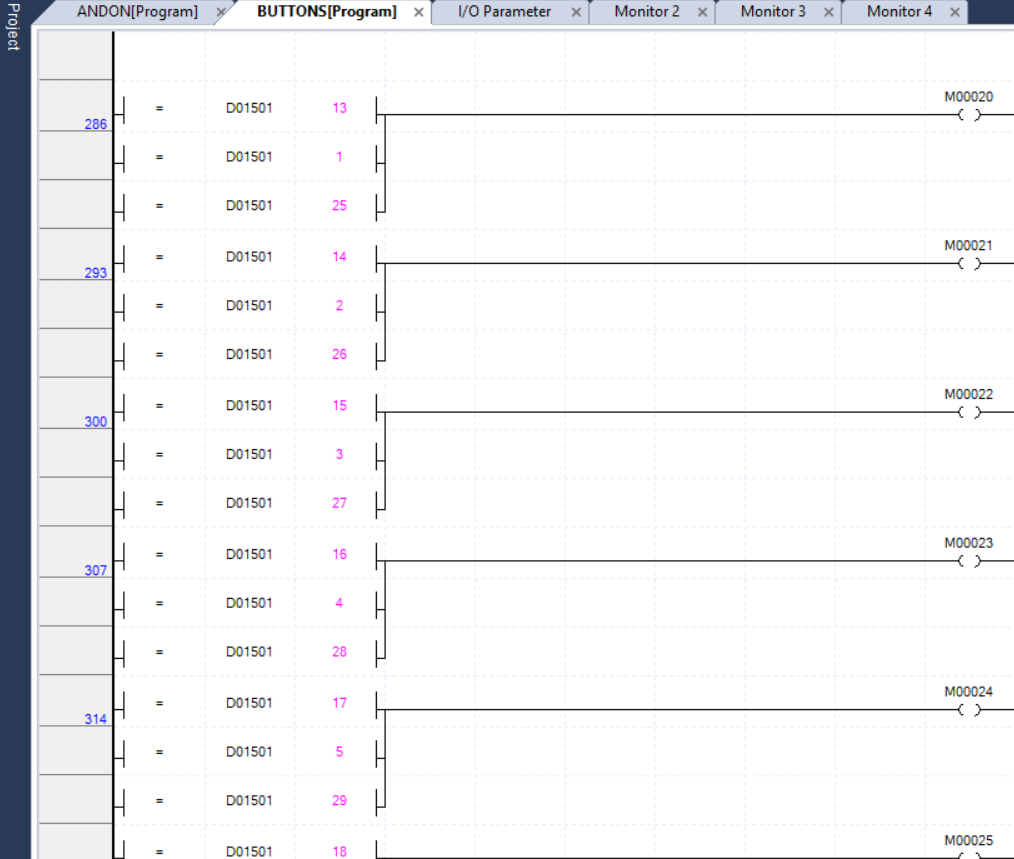
\includegraphics[width=0.72\textwidth]{Imagens/clp_08_buttons_marcas.png}
    \caption{BUTTONS: conversão dos estados em marcas; \cod{M00020} ativa em 1, 13 ou 25. (arquivo: Imagens/clp\_08\_buttons\_marcas.png)}
\end{figure}

\begin{figure}[H]
    \centering
    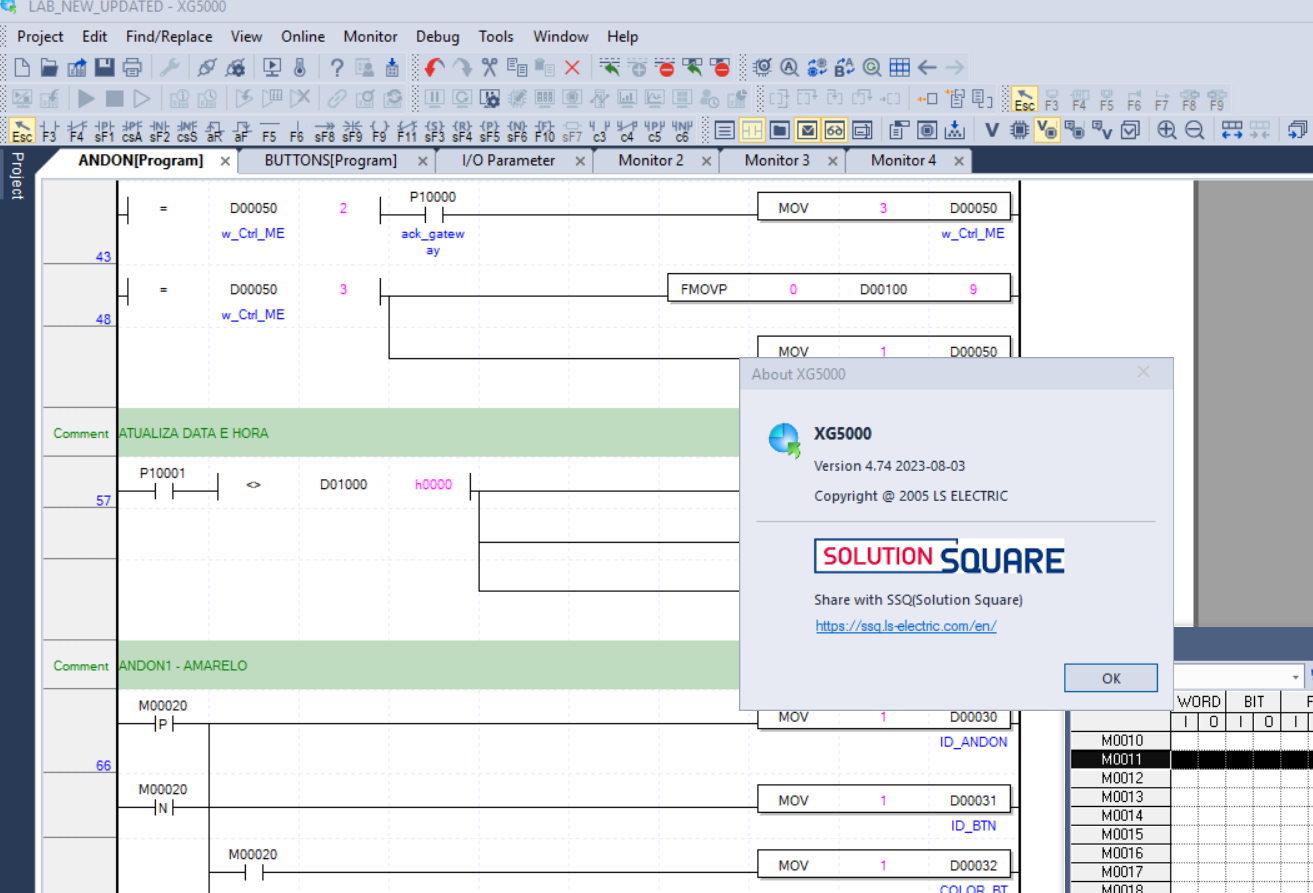
\includegraphics[width=0.72\textwidth]{Imagens/clp_03_versao_xg5000.png}
    \caption{Janela \textit{About XG5000}: versão 4.74. (arquivo: Imagens/clp\_03\_versao\_xg5000.png)}
\end{figure}

\begin{figure}[H]
    \centering
    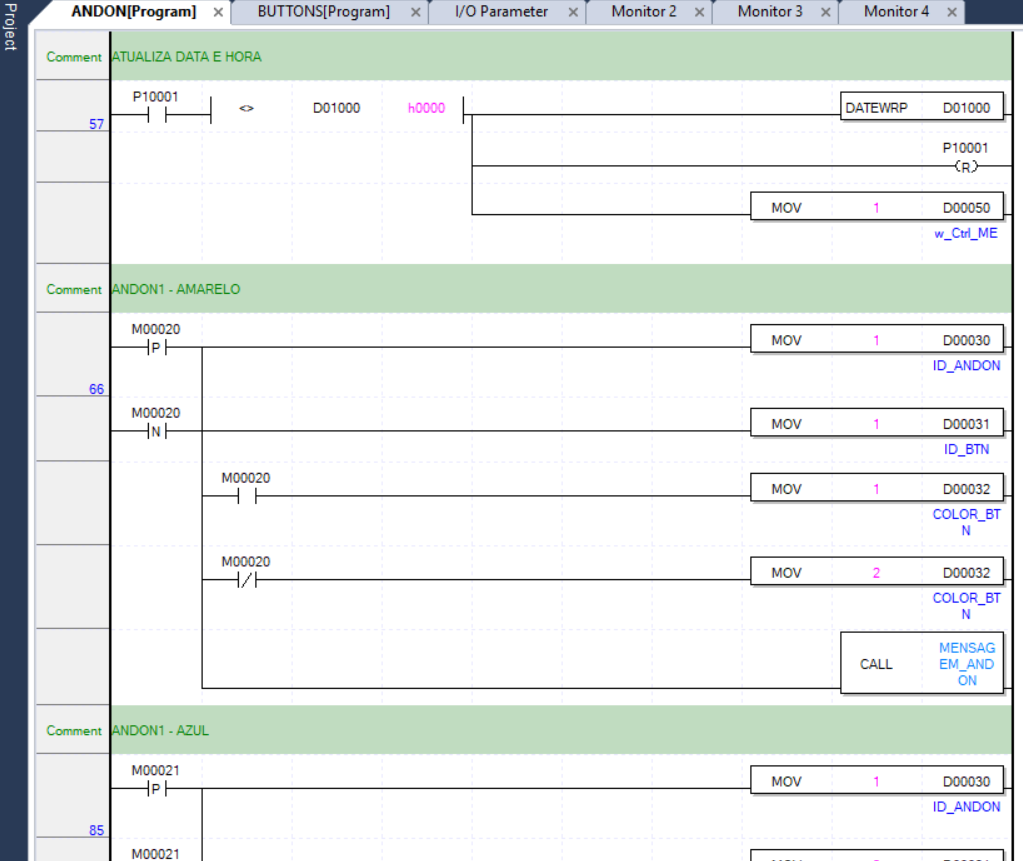
\includegraphics[width=0.72\textwidth]{Imagens/clp_11_andon_relogio_amarelo.png}
    \caption{ANDON: aplicação do relógio (\cod{P10001} e \cod{DATEWRP D01000}) e rede do Andon amarelo. (arquivo: Imagens/clp\_11\_andon\_relogio\_amarelo.png)}
\end{figure}

\begin{figure}[H]
    \centering
    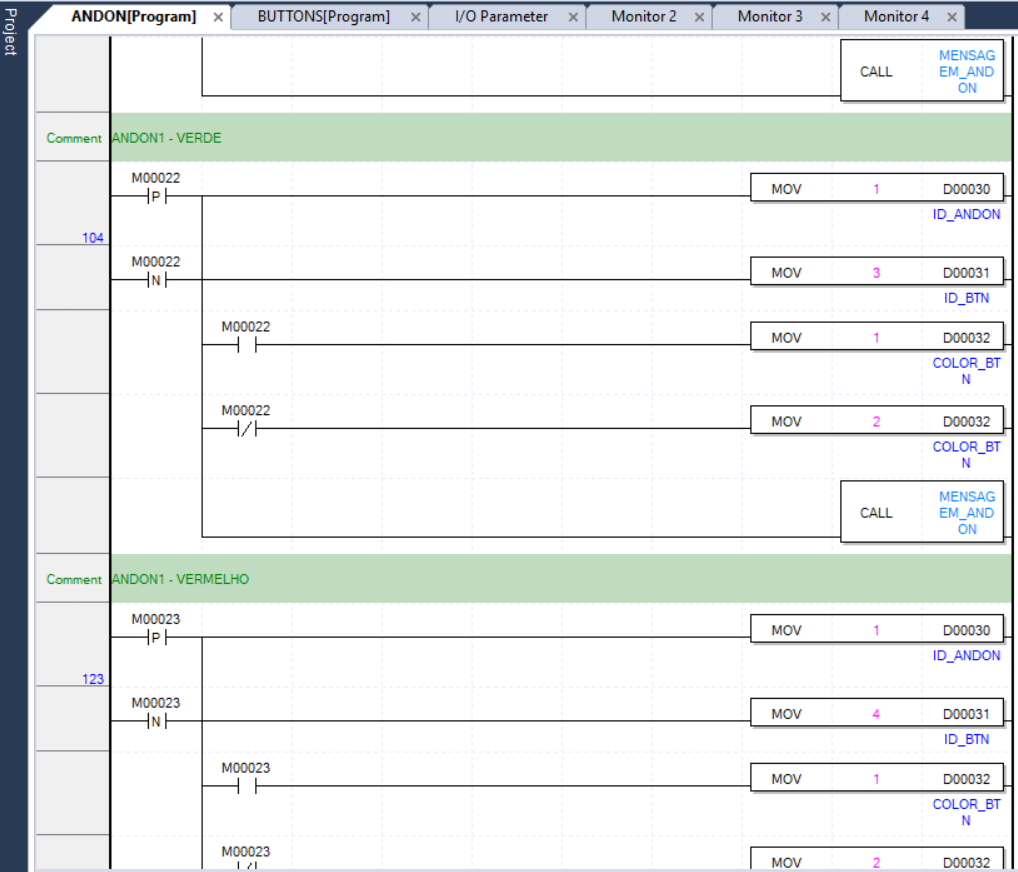
\includegraphics[width=0.72\textwidth]{Imagens/clp_12_andon_verde_vermelho.png}
    \caption{ANDON: redes dos Andons verde e vermelho. (arquivo: Imagens/clp\_12\_andon\_verde\_vermelho.png)}
\end{figure}

\begin{figure}[H]
    \centering
    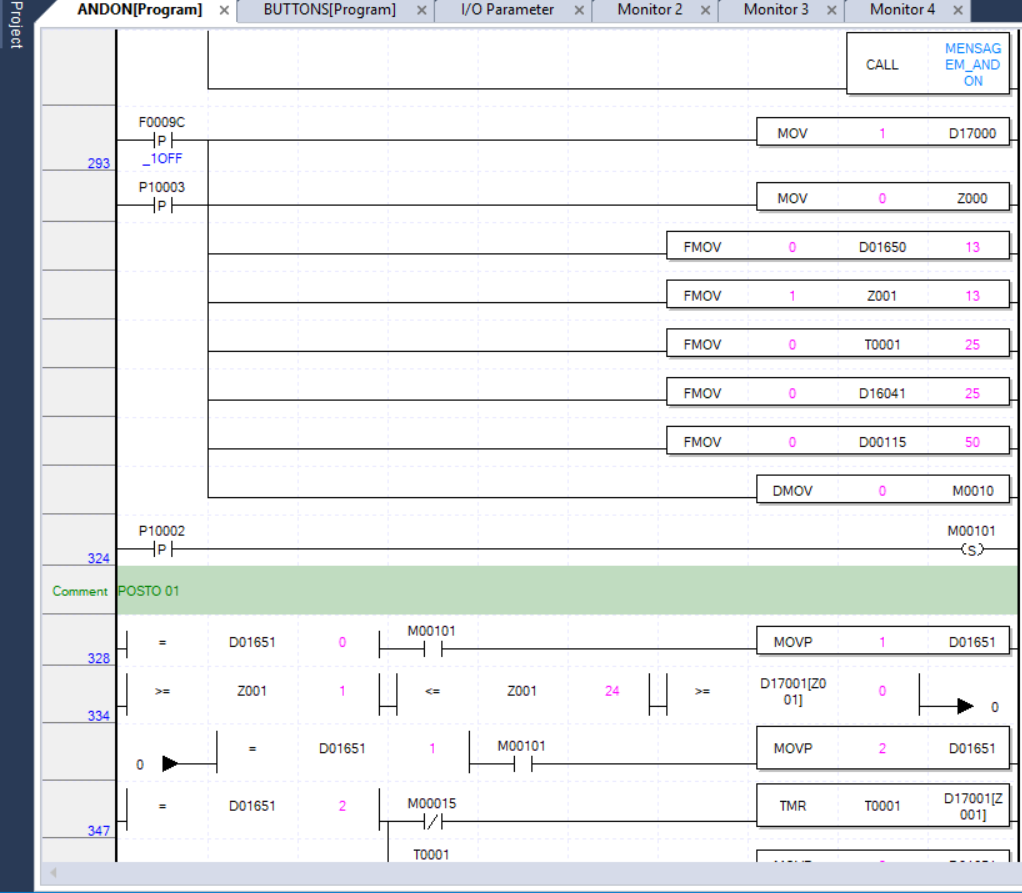
\includegraphics[width=0.72\textwidth]{Imagens/clp_14_inicializacao_start_reset.png}
    \caption{Redes de reset (\cod{P10003}) e Start (\cod{P10002} $\rightarrow$ \cod{M00101}). (arquivo: Imagens/clp\_14\_inicializacao\_start\_reset.png)}
\end{figure}

\begin{figure}[H]
    \centering
    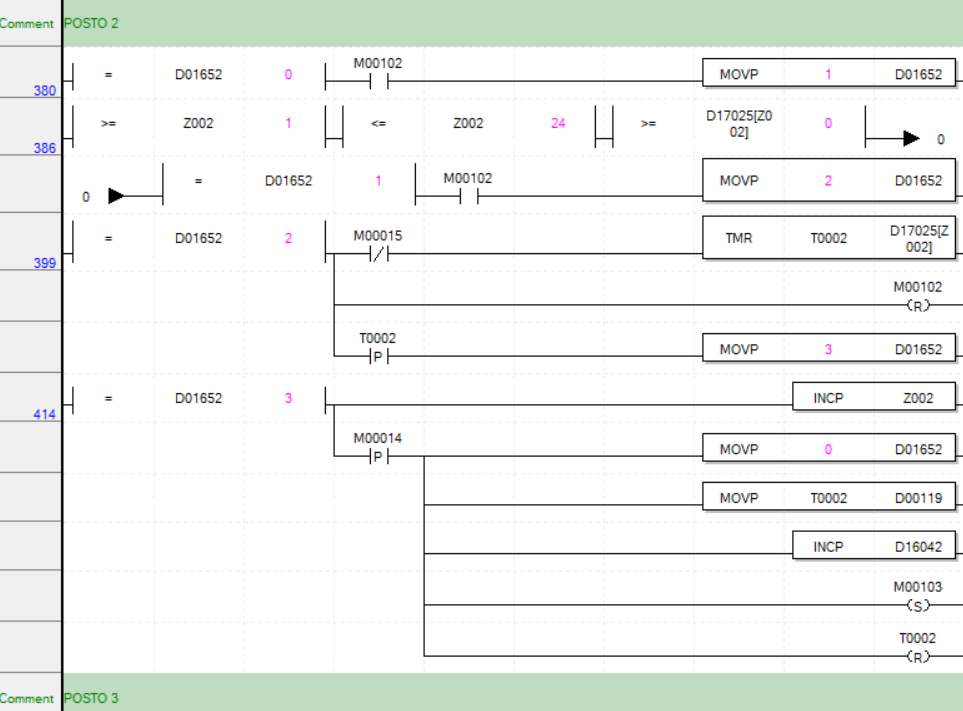
\includegraphics[width=0.72\textwidth]{Imagens/clp_16_posto_02.png}
    \caption{Posto 02: \cod{D01652}, \cod{T0002} e incremento de \cod{D16042}. (arquivo: Imagens/clp\_16\_posto\_02.png)}
\end{figure}

\begin{figure}[H]
    \centering
    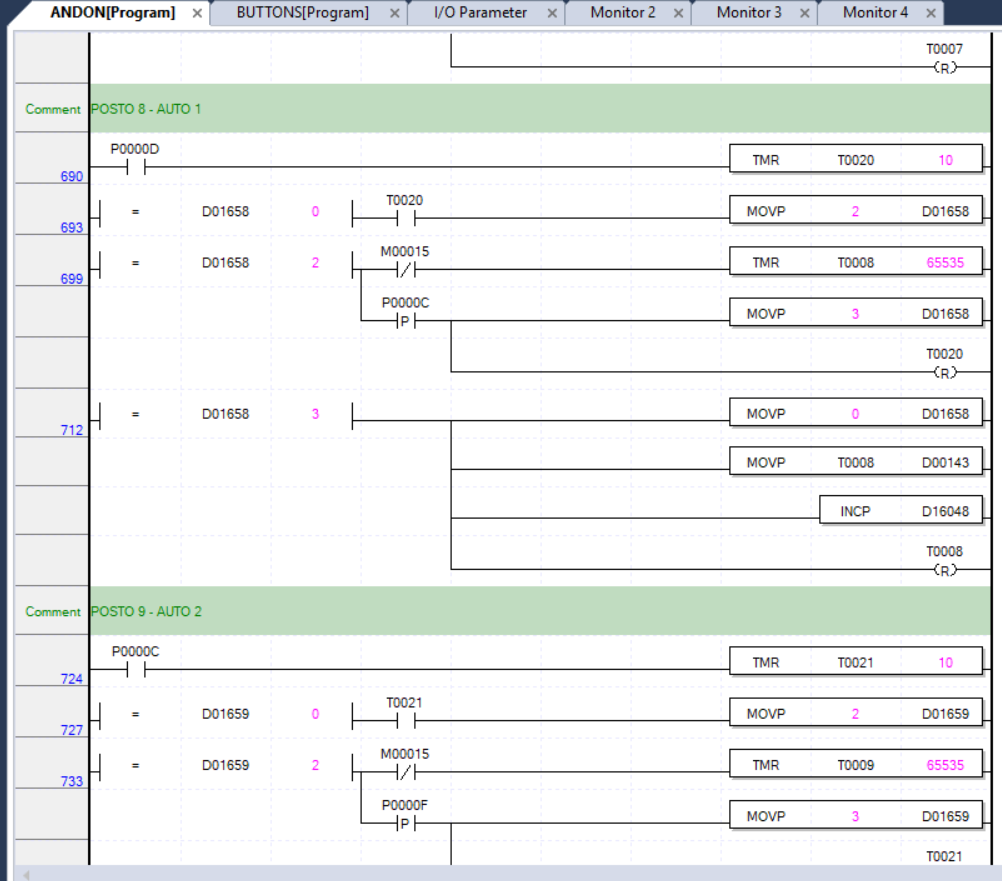
\includegraphics[width=0.72\textwidth]{Imagens/clp_18_posto_08_auto_1.png}
    \caption{Posto 08 (Auto 1): entrada por \cod{P0000D} e término pela borda de \cod{P0000C}. (arquivo: Imagens/clp\_18\_posto\_08\_auto\_1.png)}
\end{figure}

\begin{figure}[H]
    \centering
    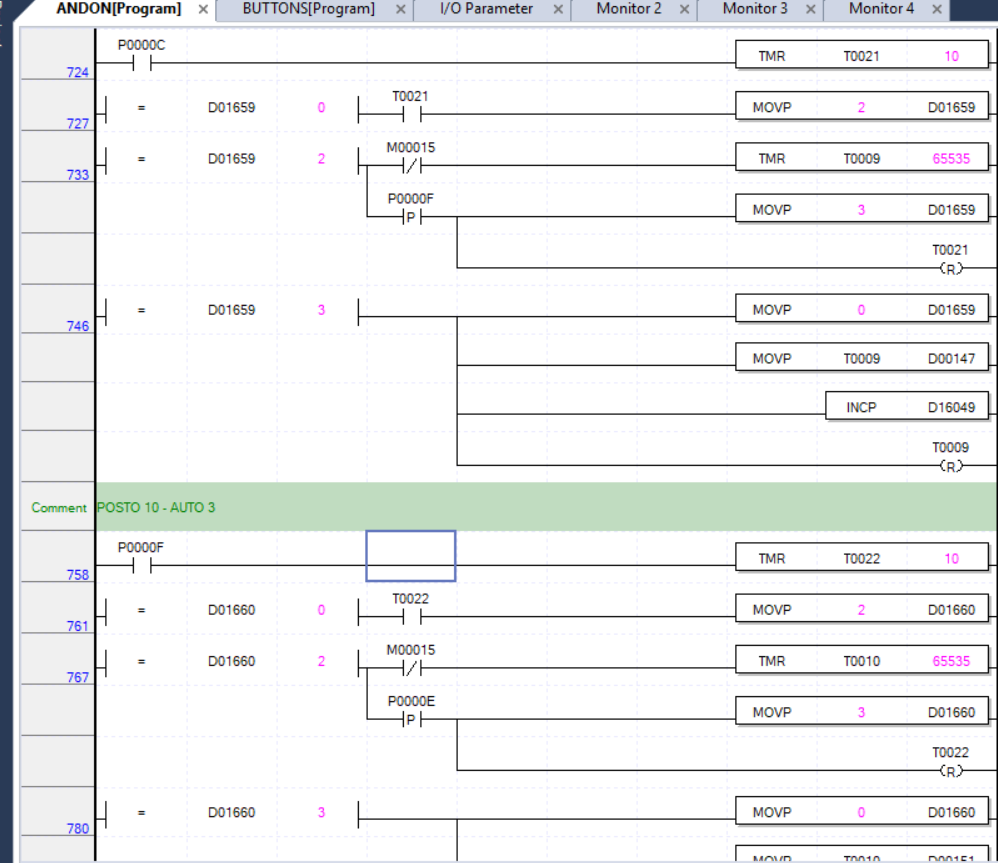
\includegraphics[width=0.72\textwidth]{Imagens/clp_19_posto_09_auto_2.png}
    \caption{Posto 09 (Auto 2): estado em \cod{D01659}; tempo de \cod{T0009} copiado para \cod{D00147}. (arquivo: Imagens/clp\_19\_posto\_09\_auto\_2.png)}
\end{figure}

\begin{figure}[H]
    \centering
    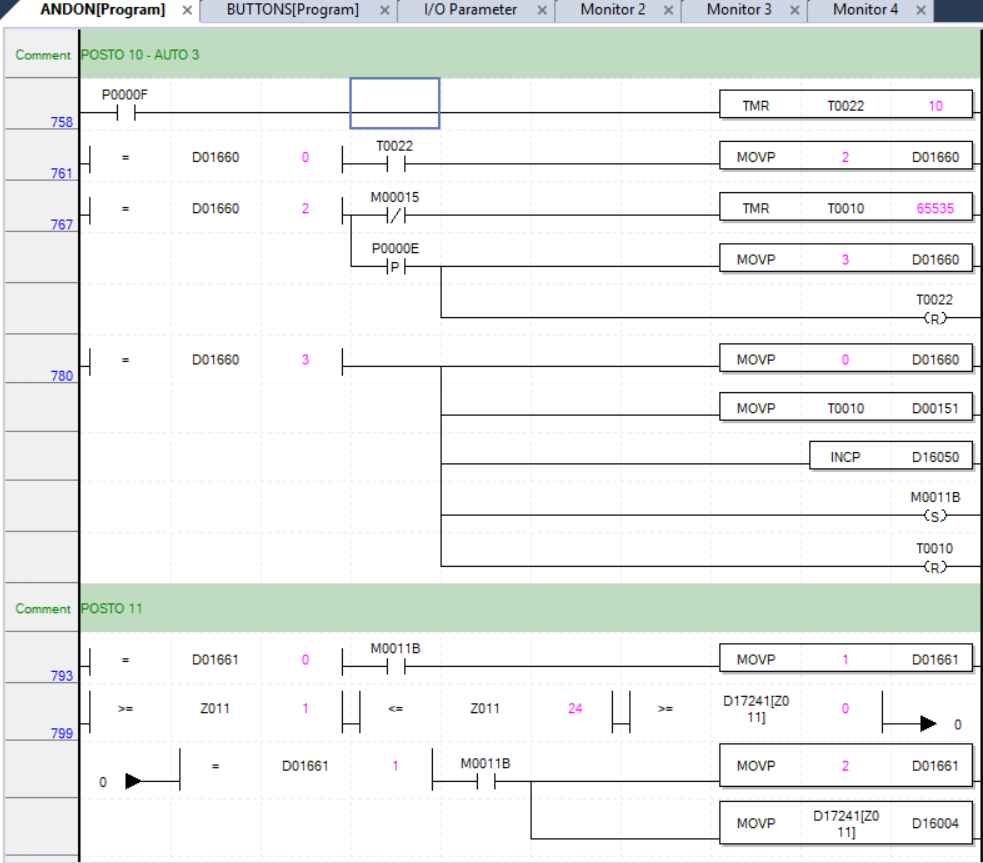
\includegraphics[width=0.72\textwidth]{Imagens/clp_20_posto_10_auto_3.png}
    \caption{Posto 10 (Auto 3): registro em \cod{D00151}, incremento de \cod{D16050} e sinal ao P11 por \cod{M0011B}. (arquivo: Imagens/clp\_20\_posto\_10\_auto\_3.png)}
\end{figure}


\end{document}
